\documentclass[11pt,a4paper,twoside]{report}
\usepackage[table]{xcolor}
\usepackage[utf8]{inputenc}
\usepackage{textcomp}
\usepackage{amsmath}
\usepackage{dsfont}
\usepackage{listings}
\usepackage{amsfonts}
\usepackage{amssymb}
\usepackage{tabularx}
\usepackage{booktabs}
\usepackage{enumitem}
\usepackage{algorithm}% http://ctan.org/pkg/algorithm
\usepackage[noend]{algorithmic}
\usepackage{parskip}
\usepackage{tikz}
\usepackage[margin=1in]{geometry}
\usepackage{graphicx}
\usepackage{hyperref}
\usepackage{epigraph}
\usetikzlibrary{arrows,fit,positioning}
\usepackage{subcaption}
\usepackage[colorinlistoftodos]{todonotes}
\usepackage[numbers]{natbib} %numbers
\usepackage{wrapfig}
\usepackage{centernot}

% this is included to get tables with colored rows to not draw over hlines and vlines
\usepackage{etoolbox}

\makeatletter
\patchcmd{\@classz}
  {\CT@row@color}
  {\oldCT@column@color}
  {}
  {}
\patchcmd{\@classz}
  {\CT@column@color}
  {\CT@row@color}
  {}
  {}
\patchcmd{\@classz}
  {\oldCT@column@color}
  {\CT@column@color}
  {}
  {}
\makeatother


\usepackage{amsthm}

\graphicspath{ {figures/} }
\pgfarrowsdeclarecombine{ring}{ring}{}{}{o}{o}

\DeclareMathOperator{\ringarrow}{\raisebox{0.5ex}{\tikz[baseline]{\draw[ring->](0,0)--(2em,0);}}}
\DeclareUnicodeCharacter{00A0}{ }




\tikzset{
    %Define standard arrow tip
    >=stealth',
    %Define style for boxes
    punkt/.style={
           circle,
           rounded corners,
           draw=black, thick,
           text width=1em,
           minimum height=1em,
           text centered},
    observed/.style={
           circle,
           rounded corners,
           draw=black, thick,
           minimum width=2.3em,
           minimum height=2.3em,
           font=\footnotesize,
           text centered,
           fill=black!10!white
           },
     latent/.style={
           circle,
           rounded corners,
           draw=black, thick, dashed,
           minimum width=2.2em,
           minimum height=2.2em,
           font=\footnotesize,
           text centered
           },
    target/.style={
           circle,
           rounded corners,
           draw=black, thick,
           minimum width=2.2em,
           minimum height=2.2em,
           font=\footnotesize,
           text centered,
           fill=black!20!white,
           },
    observedrect/.style={
           rectangle,
           rounded corners,
           draw=black, thick,
           minimum width=6em,
           minimum height=2em,
           font=\footnotesize,
           text centered,
           fill=black!10!white
           },
    latentrect/.style={
           rectangle,
           rounded corners,
           draw=black, thick, dashed,
           minimum width=2.2em,
           minimum height=2.2em,
           font=\footnotesize,
           text centered
           },
     targetrect/.style={
           rectangle,
           rounded corners,
           draw=black, thick,
           minimum width=6em,
           minimum height=2em,
           font=\footnotesize,
           text centered,
           fill=black!20!white,
           },
     empty/.style={
           circle,
           rounded corners,
           minimum width=.5em,
           minimum height=.5em,
           font=\footnotesize,
           text centered,
           },
    % Define arrow style
    pil/.style={
           o->,
           thick,
           shorten <=2pt,
           shorten >=2pt,},
    sh/.style={ shade, shading=axis, left color=red, right color=green,
    shading angle=45 }   
}





\newcommand{\KL}{\operatorname{KL}}

\newcommand{\Pij}[1]{\operatorname{P}_{ij}\!\left\{#1\right\}}
\newcommand{\Pkl}[1]{\operatorname{P}_{kl}\!\left\{#1\right\}}
\newcommand{\Q}[1]{\operatorname{Q}\left(#1\right)}
\newcommand{\EE}{\mathbb E}
\newcommand{\EEa}{\EE_a}
\newcommand{\Pns}[2]{\operatorname{P}_{#1}\left\{#2\right\}}
\newcommand{\Pn}[2]{\operatorname{P}\left\{#2|#1\right\}}
\newcommand{\actions}{\mathcal{A}}
\newcommand{\calA}{\mathcal A}
\newcommand{\etc}{\textit{etc}}
\newcommand{\ie}{\textit{i.e.}}
\newcommand{\eg}{\textit{e.g.}}
\newcommand{\calP}{\mathcal P}
\newcommand{\x}{\boldsymbol{x}}
\newcommand{\Ps}{\operatorname{P}}
\newcommand{\R}{\mathbb R}
\newcommand{\Pri}[1]{\operatorname{P}_i\left\{#1\right\}}
\newcommand{\Prz}[1]{\operatorname{P}_0\left\{#1\right\}}
\newcommand{\indep}[1]{\mathcal{I}\left(#1\right)}
\newcommand{\vb}[1]{\boldsymbol{#1}}
\newcommand{\card}[1]{\left\vert{#1}\right\vert}
\newcommand{\actionspace}{\mathcal{A}}


\newcommand{\V}[1]{\mathbb V\left[#1\right]}
\newcommand{\Esub}[2]{\mathbb E_{#1}\left[{#2}\right]}
\newcommand{\defined}{\vcentcolon =}
\newcommand{\rdefined}{=\vcentcolon}
\newcommand{\E}[1]{\mathbb E\left[{#1}\right]}
\newcommand{\Var}{\operatorname{Var}}
\newcommand{\calF}{\mathcal F}
\newcommand{\sr}[1]{\stackrel{#1}}
\newcommand{\set}[1]{\left\{#1\right\}}
\newcommand{\ind}[1]{\mathds{1}\!\!\set{#1}}

\newcommand{\argmax}{\operatornamewithlimits{arg\,max}}
\newcommand{\argmin}{\operatornamewithlimits{arg\,min}}
\newcommand{\floor}[1]{\left \lfloor {#1} \right\rfloor}
\newcommand{\ceil}[1]{\left \lceil {#1} \right\rceil}
\newcommand{\eqn}[1]{\begin{align}#1\end{align}}
\newcommand{\eq}[1]{\begin{align*}#1\end{align*}}
\newcommand{\Ber}{\operatorname{Bernoulli}}
\newcommand{\bigo}[1]{\mathcal{O}\left( #1 \right)}
\newcommand{\bigotilde}[1]{\tilde{\mathcal{O}}\left( #1 \right)}
\newcommand{\bigtheta}[1]{\Theta\left( #1 \right)}
\newcommand{\bigthetatilde}[1]{\tilde{\Theta}\left( #1 \right)}
\newcommand{\bigomega}[1]{\Omega\left( #1 \right)}

\renewcommand{\P}[1]{\operatorname{P}\left(#1\right)}
\newcommand{\cf}[2]{{#1}^{#2}}
\newcommand{\cfb}[2]{{#1}_t^{#2}} % used to represent reward
\newcommand{\bernoulli}{\operatorname{Bernoulli}}
\newcommand{\dirac}{\operatorname{Dirac}}
\newcommand{\parents}[1]{\operatorname{\mathcal{P}a}_{#1}}
\renewcommand{\vec}[1]{\boldsymbol{#1}}
\newcommand{\regret}{\bar{R}_{T}} %psuedo-regret
\newcommand{\expectedregret}{\mathbb{E}R_{T}} % expected regret
\newcommand{\rawregret}{R_{T}} % plain regret
\newcommand{\simpleregret}{R_T}
\newcommand{\quotes}[1]{``#1''}

\theoremstyle{plain} 
\newtheorem{theorem}{Theorem}
\newtheorem{proposition}[theorem]{Proposition}
\newtheorem{lemma}[theorem]{Lemma}
\newtheorem{corollary}[theorem]{Corollary}

\theoremstyle{definition}
\newtheorem{definition}[theorem]{Definition}
\newtheorem{assumption}[theorem]{Assumption}
\newtheorem{remark}[theorem]{Remark}
\newtheorem{example}[theorem]{Example}
\let\temp\epsilon
\let\epsilon\varepsilon

\newcommand{\ci}{\mathrel{\perp\mspace{-10mu}\perp}}
\newcommand{\nci}{\centernot{\ci}}


\author{Finnian Lattimore}
\title{Learning how to act: making good decisions with machine learning}

\setcounter{secnumdepth}{3}

\begin{document}

%\def\ci{\perp\!\!\!\perp} % from Wikipedia

\begin{titlepage}
    \begin{center}
        \vspace*{1cm}
        
        \Huge
        {Learning how to act: making good decisions with machine learning}
        
        \vspace{2cm}
        \Large
        {Finnian Lattimore}
        
        \vfill
        \Large
        A thesis submitted for the degree of Doctor of Philosophy
         
         The Australian National University
        
        \vspace{1cm}
        
        September 2017
        
    \end{center}
\end{titlepage}


\epigraph{In vain the grave, with retrospective Eye,
Would from the apparent what conclude the why,
Infer the Motive from the Deed, and show
That what we chanced, was what we meant, to do.}{Alexander Pope}



\clearpage
\vspace*{\fill}
\begin{center}
\begin{minipage}{.9\textwidth}
Except where acknowledged in the customary manner, the material 
presented in this thesis is, to the best of my knowledge, original and has not been submitted in whole or part for a degree in any 
university.

\vspace{40mm}  % vertical space

\hspace{80mm}\rule{40mm}{.15mm}\par   % horizontal space, line, start new line
\hspace{80mm} Finnian Lattimore\par
\hspace{80mm} September, 2017
\end{minipage}
\end{center}
\vfill % equivalent to \vspace{\fill}
\clearpage

\begin{abstract} 

This thesis is about machine learning and statistical approaches to decision making. How can we learn from data to anticipate the consequence of, and optimally select, interventions or actions? Problems such as deciding which medication to prescribe to patients, who should be released on bail, and how much to charge for insurance are ubiquitous, and have far reaching impacts on our lives. There are two fundamental approaches to learning how to act: reinforcement learning, in which an agent directly intervenes in a system and learns from the outcome, and observational causal inference, whereby we seek to infer the outcome of an intervention from observing the system. 

The goal of this thesis to connect and unify these key approaches. I introduce causal bandit problems: a framework that combines causal graphical models, which were developed for observational causal inference, with multi-armed bandit problems, which are a subset of reinforcement learning problems that are simple enough to admit formal analysis. I show that knowledge of the causal structure allows us to transfer information learned about the outcome of one action to predict the outcome of an alternate action, yielding a novel form of structure between bandit arms that cannot be exploited by existing algorithms. I propose an algorithm for causal bandit problems and prove bounds on the simple regret demonstrating it is close to mini-max optimal and strictly better than algorithms that do not use the additional causal information. 

\end{abstract} 

%\chapter*{Acknowledgements}  





\tableofcontents


\chapter{Introduction}

\section{Motivation}
Many of the most important questions in science, commerce and our personal lives are about the outcomes of doing something. Will asking people to pay upfront at the doctors reduce long term health expenditure? If we developed a drug to suppress particular genes, could we cure multiple sclerosis and would delaying teen-aged pregnancies improve the outcome for their children.  

These are hard questions because they require more than identifying a pattern in data. Correlation is not causation. Causal inference has proven so difficult that there is barely any consensus on even enduring questions like the returns to education or the long-term consequences of early life events – like teenage pregnancy, despite the fact that the variables involved are susceptible to human intuition and understanding. 

We now live in a world of data. Hours of our lives are spent online, where every click can be recorded, tiny computers and sensors are cheap enough to incorporate into everything and where the US Institute of Health is considering if all infants should be genetically sequenced at birth. Such data gives us a window into many aspects of our lives at an unprecedented scale and detail but it is messy, complicated and often generated as a by-product of some other purpose. It does not come from the controlled world of a randomised experiment.

The rise of big data sets and powerful computers has seen an explosion in the application of machine learning. From health care, to entertainment and self-driving cars, machine learning algorithms will transform many industries. It has been suggested that the impressive ability of statistical machine learning to detect complex patterns in huge data sets heralds the end of theory \citep{anderson2008end} and that we may be only a short step from \quotes{The Singularity}, where artificial intelligence exceeds our own and then grows exponentially. 

However, despite the huge advances in machine learning (in particular deep learning), machine learning algorithms are effective only within narrow problem settings. Getting them to generalise to even slightly different problems or data sets remains very challenging. Deciding how we should act or what policies we should implement requires predictions about how a system will behave if we change it. The correlations detected by standard machine learning algorithms do not enable us to do this, no matter how many petabytes of data they are based on. As machine learning algorithms are incorporated into more and more of the decision making processes that shape the world we live in, it is critical to ensure we understand the distinction between causality and prediction and that we develop techniques for learning how to act that are as effective as those we have for pattern recognition.


\section{What is causality? }

The notion of causality has been widely debated in science and philosophy \citep{hume1741treatise,mill1893system,pearson1911grammar,Pearl2000,Lewis2000,woodward2005making,heckman20051,cartwright2007hunting} but is still widely viewed as poorly defined. This has led to a reluctance among applied researchers in many fields to make concrete claims about causality in their work, leading them instead to report that variables are \textit{related}, \textit{correlated} or \textit{associated}. However, the magnitude, direction and even existence of an association depends which variables are controlled for (or included in a regression). Avoiding formalising causation, which is the real question of interest, requires the reader to determine via \quotes{common sense} the implications of the reported associations.

There are two ways in which an association detected in a data set may be non-causal. The first is that the variables concerned may not be related at all, and the association has arisen by chance in that data sample. Given a finite data on enough variables, there is a high probability of finding some that appear correlated even though they are completely unrelated. For example, based on data from the years 1999 to 2009, the age of Miss America is strongly correlated with the number of murders  (in the US) by steam, hot vapours and hot objects \citep{Vigen2015}. We would not expect this relationship to hold in a new sample of data. This form of spurious correlation also has serious repercussions. It lies at the heart of major problems with the process of scientific research: researchers are incentivised to detect effects and thus to explore many possible paths in the process of analysing data and studies that fail to find an effect are less likely to be published. Consequently, the likelihood that reported effects have arisen by chance is underestimated, leading to the conclusion that \quotes{most published scientific results are false} \citep{Ioannidis2005}. This issue is also highlighted by recent crises in replication \citep{OpenScienceCollaboration2015}. This issue can be ameliorated by obtaining more data and by separating learning models from evaluating their performance, for example by evaluating models on a strict hold-out set or on the extent to which their results can be replicated. 

However, a strong association, observed in multiple independent studies may still not be causal. The correlation can arise because both variables are consequences of some other, unmeasured factor. For example, the reading ability of children under twelve is strongly correlated with their height, because older children are taller and can read better. However height is not a cause of reading ability because interventions to increase a child's height, for example by giving them growth hormones, would not be expected to improve their reading. Similarly, extra lessons in reading will not make a child grow taller. This problem is fundamentally different to the issue of spurious correlations arising by chance in finite data sets. Obtaining more (even infinitely many more) samples without directly intervening in the system to manipulate the variables does not allow us to separate causation from correlation. 

The key distinction between a real, but non-causal, association and a causal relationship is in what happens if we intervene in the system and change one of the variables. In this thesis, I take an interventionist viewpoint of causality: any model or approach designed to predict the outcome of intervening in a system is causal. This viewpoint captures the types of questions that motivate this thesis. How can we change the way we do things to obtain better outcomes? 

Causality is often liked to explanation; understanding how and why things happen. I view explanation in terms of compression and generalisabilty: the amount of information about the world a model can capture. This creates a hierarchy in the degree to which models are explanatory, rather than a simple binary distinction. A standard predictive model encodes all the information needed to predict some output given inputs provided the system generating the data does not change. A high-level causal model might be able to predict the outcome of a specific intervention holding all else fixed. More detailed causal models could predict the outcome for a wide range of combinations of interventions conditional on a range of contexts. By considering conditional interventions within our definition of causal questions we also capture mediation: the study of pathways through which one variable causes another \cite{vanderweele2015explanation}. Finally, a model that can distil how elements interact into mathematical equations like Newton's laws can be used to predict what will happen in an astounding range of settings, including many never previously observed \footnote{Although Newton's laws are not fully general, as they break down for extremely massive objects}.

\citet{Gelman2010,gelman2013ask} make a distinction between forward causal inference, the types of \quotes{what if} questions I focus on in this thesis, and reverse causal questions, asking why something occurs. The former aims to identify the effect of a known cause. The latter can be viewed as identifying causes of an effect. They regard forward causal inference as well defined within the counterfactual and graphical model frameworks for causal inference, that we describe in section \ref{sec:causal_models}. However, they state that \quotes{A reverse causal question does not in general have a well-defined answer, even in a setting where all possible data are made available.} I view this as overly pessimistic, depending on how \quotes{all possible data} is defined. The goal of identifying the causes of an effect can be formalised within the graphical causal model framework. Solving this problem is certainly much more challenging than identifying the effect of a specific intervention on a given outcome, since it requires us to test or infer the effect of interventions on many different variables. These practical difficulties may well be overwhelming, particularly in fields such as social science and economics where data sets are often relatively small, systems are complex, the variables are difficult to directly manipulate and even relatively simple "what if" questions are hard to resolve conclusively. However, this does not mean that the problem of identifying causes of effects is ill-posed in principle. It can be viewed as a form of causal discovery: the attempt to learn the structure of the causal relationships between variables, on which there is a rich literature, see for example \citep{}.
\todo{reference a review paper on causal discovery here}

There has traditionally been a large gap between researchers in machine learning who focus on prediction, using largely non-interpretable models and researchers in statistics, social science and economics who (at least implicitly) aim to answer causal questions and tend to use highly theory-driven models. However, there is relatively little awareness, particularly within the machine learning and data science communities, of what constitutes a causal problem and the implications of this for the training and evaluation models. In the next section we emphasise the subtly that can exist in determining if a problem is causal by examining some typical examples. 

\section{What makes a problem causal?}

Machine learning is in the midst of a boom, driven by the availability of large data sets and the computation resources to process them. Machine learning techniques are being applied a huge range of problems, in both industry and academia. The following examples are intended to capture the breadth of problems that machine learning algorithms are actively being applied to. Which, if any, of these problems require causal inference? 

\begin{itemize}
\item Speech recognition (for systems like Siri or Google Assistant)
\item Image classification
\item Forecasting the weather
\item Identifying spam emails
\item Automated essay marking
\item Predicting the risk of death in patients with pneumonia.
\item Predicting who will re-offend on release from prison 
\item Customer churn modelling
\item Demand prediction for inventory control
\item Playing Go 
\end{itemize}

The question is disingenuous because I have not posed the problems in sufficient detail to determine if causality is an important consideration. In particular, I failed to specify how any model we might build would be used: what actions would be taken in response to its predictions. 

Consider speech recognition. You say something, which causes sound waves, which are converted to a digital signal that Siri maps to words. Whatever action Siri takes is unlikely to change the distribution of words you use, and even less likely to change the function that maps sound waves to text (unless she sends you a DVD on elocution). A similar argument could be made for many applications of machine translation and image classification. 

In image classification we do not particularly care about building a strong model for exactly how the thing that was photographed translates to an array of pixels, provided we can be fairly confident that the process will not change. If we develop a discriminative model that is highly accurate at classifying cats from dogs, we do not need to understand its internal workings (assuming we have strong grounds to believe that the situations in which we will be using our model will match those under which it was trained).

What about forecasting the weather? If you are using a short term forecast to decide whether to pack an umbrella, causality can be ignored. Your decision will not affect if it actually rains. However, longer term climate forecasts might (theoretically) lead to action on emissions which would then change the weather system. For this we need a (causal) model that allows us to predict the outcome under various different interventions.

Identifying spam and automated essay marking both involve processing text to determine an underlying (complex) attribute such as its topic or quality. In both cases, there is inherent competition between the algorithm and the people generating the text. As a result, decisions made by the algorithm are likely to change the relationship between the features it relies on and the true label. Spammers and students will modify their writing in order to optimise their results. A standard supervised learning approach can only work if the resulting change in the mapping from features to label is sufficiently gradual. There are two key ways of ensuring this. The first is to limit people's ability to observe (and thus react to) decisions made by the algorithm. The second is to use a model in which the features are related to the outcome in such a way that they cannot be manipulated independently. 

This example also highlights a connection between causal models and transparency in machine learning. If we are using a non-causal model to make decisions affecting people, there will be a trade-off between the performance and transparency of the model; not because the requirement for transparency restricts us to simple models, but because revealing how the model works allows people to change their behaviour to game it. 

What about predicting the risk of death in patients with pneumonia? Suppose the goal is to build a model to decide who should be treated in hospital and who can be sent home with antibiotics. If we assume that in hospital treatment is more effective for serious cases, this appears to be straightforward prediction. It is not. Depending on how the decision to admit was previously made and what features are included (or omitted) in the model, the relationship between those features and the outcome may change if the model is used to make admission decisions. \citet{Caruana2015} found exactly this effect in a real data set. The model learned that people suffering asthma were \emph{less} likely to die from pneumonia. This was because doctors treated such patients very aggressively, thus actually lowering their risk. The issue is not with model; it performed very well at the task for which it was trained, which is to predict who would be likely to die under the original admission and treatment protocols. However, using it to decide how to \emph{change} these protocols could kill. The actual question of interest in this case is what happens to patients with characteristics $X$ they are assigned treatment according to decision rule (or policy) $\pi(X)$. 

Predicting recidivism among paroled prisoners or customer churn also fit within the class of problems where the goal is to identify a group for which a problem will occur in order to target treatment (additional support and monitoring for people on parole, loyalty rewards to improve customer retention, hospitalisation for the severely ill). Predictive models can be applied to such problems where the most effective treatment is known for a given target group, and where deciding who to treat on the basis of the model predictions will not change the relationship between the features and outcome.

Predicting which customers will leave or who will re-offend if granted parole also fit within the category of problems where you wish to identify a group for which a problem will occur and target some treatment to them (hospitalisation, loyalty reward, more monitoring \& support on parole, etc). Predictive models can be applied to such problems provided it is known which treatment option will be most effective for the target group and deciding who to treat on the based of the model predictions won't change the relationship between features and outcome.

Demand prediction seems like a relatively straightforward prediction problem. Models use features such as location, pricing, marketing, time of year and weather, to forecast the demand for a product. It seems unlikely that using the model to ensure stock is available will itself change demand. However, depending on the way demand is measured, there is a potential data censoring issue. If demand is modelled by the number of sales, then if a product is out of stock demand will appear to be zero. Changing availability does then change demand.
   
Playing Go (and other games) is a case with some subtleties. At every turn, the AI agent has a number of actions available. The state of the board following each action is deterministic and given by the rules of the game. The agent can apply supervised machine learning, based on millions of previous games, to estimate the probability that each of these reachable board states will lead to a win \footnote{This is a challenging pattern recognition problem. There are around $2 \times 10^{170}$ legal board positions in Go, (\citep{tromp2016number}), so the algorithm cannot simply memorise the proportion of times each state leads to a win. It must identify higher level features of the board state that are associated with winning.}. Supervised learning can also be applied to learn a policy $\P{a|s}$, the probability of a player selecting action $a$, given board state $s$. This allows the agent to estimate the likelihood of winning from a given starting state by simulating many times the remainder of the game, drawing actions from $\P{a|s}$ for both players. Google's Alpha Go, which in May 2017 beat the then strongest human player \citep{Mozur2017}, incorporates a combination of these approaches \citep{silver2016mastering}. The supervised learning was enhanced by having the agent play (variants) of itself many times, so that its estimates of value for each board state and of the likelihood an opponent will play a given move are based on a combination of replicating the way humans play and on the moves that led to a win when playing itself. 

The problem of playing go is causal from the interventionalist perspective. The agent wishes to learn the probability of a win given an action they take. However, there are some special characteristics to the go problem that make it amenable to a primarily supervised learning approach. The actions the agent has to explore are the sames ones as human players explored to generate the training data, and both have the same objective - to win the game. In addition, the state of the board encapsulates all the information relevant to selecting a move. These factors make it reasonable to conclude that selecting moves with an algorithm will not change the value of a board state or the probability of given move by the opponent by a sufficiently large margin to invalidate the training data. 
 
Having considered these examples we can now identify some general aspects of problems that require causal (as opposed to purely predictive) inference. A predictive model may be sufficient if, given the variable(s) being predicted, it is clear which action is optimal and if selecting actions on the basis of the model does not change the mapping from features to outcomes. The second requirement is particularly difficult to satisfy when an algorithm is making important decisions affecting individual people. Think about problems like credit scoring and parole decisions. There are strong ethical grounds for demanding transparency, but if the goals of society and the individuals are not perfectly aligned and there is any possibility that people can manipulate features independently of the outcome, there will be a conflict between model accuracy and transparency. It is rare to build a model without any intent to make some kind of decision based on its results. Thus, I argue we should assume a causal model is required until we can justify otherwise.  

\section{Observe or intervene: two very different approaches to causal problems}

As we have shown, problems involving causality are ubiquitous in many fields. As a result, techniques for addressing them have developed in parallel within many disciplines, including statistics, economics, social science, epidemiology and machine learning. Although the focus and terminology can differ substantially between fields these techniques, all address the underlying goal of estimating the effect of, or optimally selecting, interventions in some system. Methods for learning about interventions can be usefully categorised into two broad approaches, reinforcement learning and observational causal inference. 

In reinforcement learning, under which we include traditional randomised experiments, we learn the outcome of actions by taking them. We take the role of an agent, capable of intervening in the system, and aim to develop algorithms that allow the agent to select actions optimally with respect to some goal. A particular strand of research within reinforcement learning are multi-armed bandit problems. They describe settings in which there are a set of available actions, the agent repeatedly decides which to select and then observes the outcome of the chosen action. They capture problems such as a doctor deciding which treatment to prescribe to a patient or a search engine selecting which advertisement to display to a user, where the agent faces the same set of choices repeatedly and is able to assess the value of outcome of the actions. 

The approach of learning the outcome of an action by taking it plays a key role in advancing our knowledge of the world. However, we frequently have access to large bodies of data that have been collected from a system in which we did not have any control over what actions were taken, or perfect knowledge of the basis on which those actions were chosen. Estimating the effect of an action from such observational data sets is the problem addressed by observational causal inference. Observational causal inference can be viewed as a form of transfer learning. The goal is to leverage data obtained from one system, the system we have observed, to estimate key characteristics of another, the system after we select an action via some policy that may differ from the process driving which actions occur in the original system. This is impossible without some assumptions about how the the original system and the system after intervention are related to one-another. The key to observational inference is to model how actions change the state of the world in such a way that we can map information collected in one setting to another. 

Both multi-armed bandits and observational causal inference can be seen as extensions to the concept of randomised controlled trials. Bandit algorithms deal with the sequential nature of the decision making process, and causal inference with problems where randomisation is not feasible, affordable or ethical. The similarities between the problems addressed by these techniques raises the question of whether there are problems best addressed by a combination of these approaches, and if so, how they can be combined. 

\section{This thesis and its contributions}

I view causal problems as one of the greatest current challenges for machine learning. They incorporate a large set of problems of huge practical significance, that require us to go beyond pattern recognition, but are well short of general artificial intelligence. For the major advances in representation and pattern recognition developed within machine learning to be effectively applied in many areas of medicine, economics, social sciences and industry, we need to understand how to leverage our improved approaches to prediction to tackle causal problems. 

\paragraph{Contributions} The goal of this thesis is to connect and unify the key approaches to solving causal problems from both the observational and interventional viewpoints. My major contribution is a framework that unifies the causal graphical model approach for inference in observational settings with the sequential experimental approach encapsulated by multi-armed bandits. This framework allows us to represent knowledge of how variables are related to one-another in a very natural way and induces an interesting and novel form of structure between the different actions modelled in the bandit problem. I develop a new algorithm that can exploit this structure as a first step towards a unified approach to decision making under uncertainty. 
I make a number of additional connective contributions that are not encompassed by my work on causal bandit problems. I demonstrate the role of a formal causal framework within Bayesian approaches to inference and show how assigning a prior based on human causal intuition without considering the causal structure of the problem can introduce bias. I highlight the connections between approaches to off-policy evaluation in bandit problems, causal effect estimation from observational data, and covariate shift. I clarify the implicit causal structure underlying various bandit settings and the counterfactual nature of \emph{regret} - the measure by which bandit algorithms are assessed.

\paragraph{Thesis overview} This thesis is divided into three key chapters, learning from observational data, learning from interventional data and unifying the approaches. Chapter \ref{chap:causality} covers learning to act from observational data. In \S\ref{sec:causal_models}, I describe the key existing frameworks for causal inference from observational data, discuss how they relate to one-another and introduce the notation required to describe causal problems. Section \ref{sec:causal effect estimation} describes the key tools these frameworks provide that enable us to answer causal questions, in particular, the do-calculus (\S\ref{sec:do_calculus}) and, in sections \ref{sec:defining-causal-effects} and \ref{sec:causal_effect_under_ignorability}, discusses how we define causal effects, the traditional approaches to estimation and how they relate to covariate shift and off-policy evaluation. Section \ref{sec:bayesian_causality} highlights the role graphical causal models can play in Bayesian inference. 


Chapter \ref{chap:interventionalist_view} deals with interventionalist viewpoint, including traditional randomised experiments (\S\ref{sec:randomized_experiment}) and multi-armed bandit problems. In \S\ref{sec:multi-armed-bandits}, I describe the key problems and results within the bandit literature, including stochastic bandits (\S\ref{sec:stochastic-bandit}), pure exploration problems (\S\ref{sec:pure-exploitation-problems}), adversarial bandits (\S\ref{sec:adversarial-bandits}) and contextual bandits (\S\ref{sec:contextual-bandits}). I clarify the causal structure of (stochastic) contextual bandit problems in \S\ref{sec:causal-structure-contextual-bandit}. In \S\ref{sec:off-policy-evaluation}, I review the literature on off-policy evaluation for bandit problems and show how it is a somewhat special case of causal effect estimation from observational data. Finally, in section \S\ref{sec:counterfactual-nature-regret} I discuss the counterfactual nature bandit regret. 

In chapter \ref{chap:causal-bandit}, I introduce causal bandit problems: a framework that unifies causal graphical models with multi-armed bandit problems. Bandit arms are related to interventions in a causal graphical model in a very natural way: each multi-armed bandit arm (or action) corresponds to a particular assignment of values to variables within the causal graphical model. I show how the framework can be used to describe a number of existing problems that lie in the intersection between the observational and interventional approaches to causality and demonstrate how problems reduce to different flavours of bandit problem depending what information is observable and when. 

In \S\ref{sec:causal-bandit-post-action-feedback}, I focus on causal bandit problems for which the values of variables in the causal graph are observed after an action is selected. I demonstrate that this leads to a novel form of structure between the bandit arms that cannot be exploited by any existing bandit algorithms. In \S\ref{sec:simple-regret}, I describe and develop an algorithm for a special case of causal bandit problem I refer to as the \emph{parallel bandit problem}. I demonstrate via upper and lower bounds on the regret that the algorithm is close to optimal for these problems and that the introduction of the causal structure leads to substantially faster learning. In \S\ref{sec:simple-regret-general}, I develop and prove regret bounds for an algorithm that can be applied to arbitrary causal graphs, albeit with stronger assumptions on what must be known apriori, and introduce a measure that captures the underlying difficulty of causal bandit problems, which depends on the causal graph and can be viewed as an \quotes{effective number of arms}. Section \ref{sec:causal-bandit-experiments} provides experiments demonstrating the performance of these algorithms on causal bandit problems. Finally in \S\ref{sec:causal_bandit_discussion}, I discuss extensions and potential future work. 


\chapter{Learning from observational data}
\label{chap:causality}

The goal of causal inference is to learn the effect of taking an action. We can do this directly via experimental approaches, however any given agent only has a limited capacity to manipulate the world. We are generating and storing data on almost every aspect of our lives at an unprecedented rate. As we incorporate sensors and robotics into our cities, homes, cars, everyday products and even our bodies, the breadth and scale of this data will only increase. However, only a tiny fraction of this data will be generated in a controlled way with the specific goal of answering a single question. An agent that can only learn from data when it had explicit control (or perfect knowledge of) the process by which that data was generated will be severely limited. This makes it critical that we develop effective methods that enable us to predict the outcome of an intervention in some system from observing it. This is the problem of observational causal inference. 

\section{Causal models}
\label{sec:causal_models}

Observational causal inference aims to infer the outcome of an intervention in some system from data obtained by observing (but not intervening in) it. As previously mentioned, this is a form of transfer learning; we need to infer properties of the system post-intervention from observations of the system pre-intervention. Mapping properties from one system to another requires some assumptions about how these two systems are related, or other words, a way of describing actions and how we anticipate a system will respond to them. Three key approaches have emerged: counterfactuals, structural equation models and causal Bayesian networks. 

Counterfactuals \citep{Rubin1974} were developed from the starting point of generalising from randomised trials to less controlled settings. They describe causal effects in terms of differences between counterfactual variables, what would happen if we took one action verses what would happen if we took another. Counterfactual assertions can be expressed very naturally in human languages and are  prevalent in  everyday conversations; \quotes{if I had worked harder I would have got better grades} and \quotes{she would have been much sicker if she hadn't taken antibiotics}. Structural equation models have been developed and applied primarily within economics and related disciplines. They can be seen as an attempt to capture key aspects of the people's behaviour with mathematics. Questions around designing policies or interventions play a central role in economics. Thus they have transformed simultaneous equations into a powerful (though somewhat poorly formalised \citep{Pearl2000}) framework and associated set of methods for estimating causal effects. Causal Bayesian networks \citep{Pearl2000} are a more recent development and arise from the addition of a fundamental assumption about the meaning of a link to Bayesian networks. They inherit and leverage the way Bayesian networks encode conditional independencies between variables to localise the impact of an intervention in a system in a way that allows formalisation of the conditions under which causal effects can be inferred from observational data. 

An understanding of causal Bayesian networks and their properties (in particular the do calculus, see section \ref{sec:do_calculus}) is sufficient to appreciate my main technical contributions in chapter \ref{chap:causal-bandit}, as well as the importance of formal causal reasoning in Bayesian inference that I highlight in section  \ref{sec:bayesian_causality}. However, the literature on causal inference techniques remains spit between the different frameworks. Much of the recent work on estimating causal effects within machine learning, as well as widely used methodologies such as propensity scoring, are described using the counterfactual framework. Methods developed within economics, in particular instrumental variable based approaches, or those requiring parametric or functional assumptions, are often based around structural equation models. This makes it worthwhile for researchers interested in causality to develop an understanding off all these viewpoints.

In the next sections, we describe causal Bayesian networks, counterfactuals and structural equation models: the problems they allow us to solve, the assumptions they rely on and how they differ. By describing all three frameworks, how they relate to one-another, and when they can be viewed as equivalent, we will make it easier for researchers familiar with one framework to understand the others and to transfer ideas and techniques between them. However, sections \ref{sec:SEM} (Structural Equation models), and \ref{sec:unifying_causal_models} (Unifying the models) are not crucial to understanding my technical contributions and may be safely skipped by uninterested readers. In order to demonstrate the notation and formalisms each framework provides, we will use them to describe the following simple examples. 

\vspace*{.3cm}
\begin{example}
\label{exm:ranomized_experiment}
Suppose a pharmaceutical company wants to assess the effectiveness of a new drug on recovery from a given illness. This is typically tested by taking a large group of representative patients and randomly assigning half of them to a treatment group (who receive the drug) and the other half to a control group (who receive a placebo). The goal is to determine the clinical impacts of the drug by comparing the differences between the outcomes for the two groups (in this case, simplified to only two outcomes - recovery or non-recovery). We will use the variable $X$ (1 = drug, 0 = placebo) to represent the treatment each person receives and $Y$ (1 = recover, 0 = not recover) to describe the outcome. 
\end{example}

\vspace*{.3cm}
\begin{example}
\label{exm:adjusting}
Suppose we want to estimate the impact on high school graduation rates of compulsory preschool for all four year olds. We have a large cross-sectional data set on a group of twenty year olds that records if they attended pre-school, if they graduated high school and their parents socio-economic status (SES). We will let $X\in \set{0,1}$ indicate if an individual attended pre-school, $Y \in \set{0,1}$ indicate if they graduated high school and $Z \in \set{0,1}$ represent if they are from a low or high SES background respectively.\footnote{There has been substantial empirical work on the effectiveness of early childhood education including a landmark randomised trial, the Perry Preschool project, which ran from 1962-1967 \citep{weikart1970longitudinal}.}
\end{example}


\subsection{Causal Bayesian networks}

Causal Bayesian networks are an extension of Bayesian networks. A Bayesian network is a graphical way of representing how a distribution factorises. Any joint probability distribution can be factorised into a product of conditional probabilities. There are multiple valid factorisations, corresponding to permutations of variable ordering.

\eqn{
\label{eqn:cbn:joint_dist}
P(X_{1},X_{2},X_{3},...)=P(X_{1})P(X_{2}|X_{1})P(X_{3}|X_{1},X_{2})...
}

We can represent this graphically by drawing a network with a node for each variable and adding links from the variables on the right hand side to the variable on the left for each conditional probability distribution, see figure \ref{fig:bayesnet}. If the factorisation simplifies due to conditional independencies between variables, this is reflected by missing edges in the corresponding network. There are multiple valid Bayesian network representations for any probability distribution over more than one variable, see figure \ref{fig:bayesnet2} for an example. 

\begin{figure}[h]
\centering
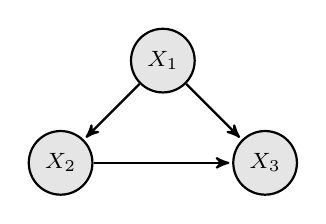
\begin{tikzpicture}[->,>=stealth',shorten >=1pt,auto,node distance=1cm,
  thick,main node/.style={observed}]

 %nodes
\node[main node](1){$X_{1}$};
\node[main node, below left=of 1](2){$X_{2}$};
\node[main node, below right=of 1](3){$X_{3}$};


 \path[every node/.style={font=\sffamily\small}]
    (1) edge node {} (2)
    	edge node {} (3)
    (2) edge node {} (3);
	
\end{tikzpicture}
\caption{A general Bayesian network for the joint distribution over three variables. This network does not encode any conditional independencies between its variables and can thus represent any distribution over three variables.}
\label{fig:bayesnet}
\end{figure}



\begin{figure}
\centering
\begin{subfigure}[t]{0.15\textwidth}
\centering
\caption{}
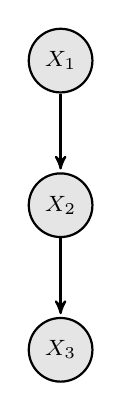
\begin{tikzpicture}[->,>=stealth',shorten >=1pt,auto,node distance=1cm, thick,main node/.style={observed}]
 %nodes
\node[main node](1){$X_{1}$};
\node[main node, below=of 1](2){$X_{2}$};
\node[main node, below=of 2](3){$X_{3}$};
\path[every node/.style={font=\sffamily\small}]
    (1) edge (2)
    (2) edge (3);
\end{tikzpicture}
\end{subfigure}
\begin{subfigure}[t]{0.15\textwidth}
\centering
\caption{}
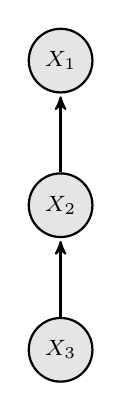
\begin{tikzpicture}[->,>=stealth',shorten >=1pt,auto,node distance=1cm, thick,main node/.style={observed}]
 %nodes
\node[main node](1){$X_{1}$};
\node[main node, below=of 1](2){$X_{2}$};
\node[main node, below=of 2](3){$X_{3}$};
\path[every node/.style={font=\sffamily\small}]
    (3) edge (2)
    (2) edge (1);
\end{tikzpicture}
\end{subfigure}
\begin{subfigure}[t]{0.3\textwidth}
\centering
\caption{}
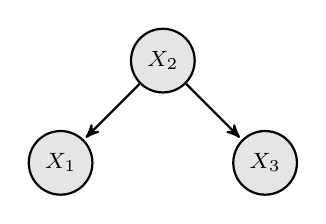
\begin{tikzpicture}[->,>=stealth',shorten >=1pt,auto,node distance=1cm, thick,main node/.style={observed}]
 %nodes
\node[main node](1){$X_{2}$};
\node[main node, below left=of 1](2){$X_{1}$};
\node[main node, below right=of 1](3){$X_{3}$};
\path[every node/.style={font=\sffamily\small}]
    (1) edge (2) edge (3);
\end{tikzpicture}
\end{subfigure}
\begin{subfigure}[t]{0.3\textwidth}
\centering
\caption{}
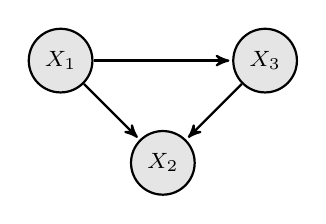
\begin{tikzpicture}[->,>=stealth',shorten >=1pt,auto,node distance=1cm, thick,main node/.style={observed}]
 %nodes
\node[main node](1){$X_{2}$};
\node[main node, above left=of 1](2){$X_{1}$};
\node[main node, above right=of 1](3){$X_{3}$};
\path[every node/.style={font=\sffamily\small}]
    (2) edge (1)
    (3) edge (1)
    (2) edge (3);
\end{tikzpicture}
\end{subfigure}
\caption{Some valid Bayesian networks for a distribution $P$ over $(X_1,X_2,X_3)$ in which $X_3$ is conditionally independent of $X_1$ given $X_2$, denoted $X_3 \ci X_1 | X_2$. Graphs (a), (b) and (c) are all a \emph{perfect map} for $P$ as the graphical structure implies exactly the same set of independencies exhibited by the distribution. Graph (d), like figure \ref{fig:bayesnet} does not imply any conditional independencies, and is thus a valid (but not very useful) Bayesian network representation for any distribution over three variables.}
\label{fig:bayesnet2}
\end{figure}


The statement that a given graph $G$ is a Bayesian network for a distribution $P$ tells us that the distribution can be factorised over the nodes and edges in the graph. There can be no missing edges in $G$ that do not correspond to conditional independencies in $P$, (the converse is not true: $G$ can have extra edges). If we let $parents_{X_{i}}$ represent the set of variables that are parents of the variable $X_{i}$ in $G$ then we can write the joint distribution as; 

\eqn{
\P{X_{1},...,X_{N}} = \prod_{i = 1...N}\P{X_{i}|parents_{X_{i}}}
}

A causal Bayesian network is a Bayesian network in which a link $X_{i} \rightarrow X_{j}$, by definition, implies $X_{i}$ causes $X_{j}$. This means an intervention to change the value of $X_{i}$ can be expected to affect $X_{j}$, but interventions on $X_{j}$ will not affect $X_{i}$. We need some notation to describe interventions and represent distributions over variables in the network after an intervention. In this thesis, I use the do operator introduced by Pearl \citep{Pearl2000}.

\vspace{0.5cm}
\begin{definition}{The do-notation}
\begin{itemize}
\item $do(X=x)$ denotes an intervention that sets the random variable(s) $X$ to $x$.
\item $\P{Y|do(X)}$ is the distribution of $Y$ conditional on an \emph{intervention} that sets $X$. This notation is somewhat overloaded. It may be used to represent a probability distribution/mass function or a family of distribution functions depending on whether the variables are discrete or continuous and whether or not we are treating them as fixed. For example, it could represent 
\begin{itemize}
\item the probability $\P{Y=1|do(X=x)}$ as a function of $x$,
\item the probability mass function for a discrete $Y$ : $\P{Y|do(X=x)}$,
\item the probability density function for a continuous  $Y$ : $f_Y(y|do(X=x))$,
\item a family of density/mass function for $Y$ parameterised by $x$.
\end{itemize}
Where the distinction is important and not clear from context we will use one of the more specific forms above. 
\end{itemize}
\end{definition}

\vspace{0.5cm}
\begin{theorem}[Truncated product formula \citep{Pearl2000}]
\label{thm:truncated_prodcut}
If $G$ is a causal network for a distribution $P$ defined over variables $X_{1}...X_{N}$, then we can calculate the distribution after an intervention where we set $Z \subset X$ to $z$, denoted $do(Z=z)$ by dropping the terms for each of the variables in $Z$ from the factorisation given by the network. Let $\parents{X_i}$ denote the parents of the variable $X_i$ in $G$.

\begin{equation}
\label{eq:truncatedproduct}
\P{X_1...X_N|do(Z=z)} = \ind{Z = z}
  \prod_{X_i \notin Z}\P{X_{i}|\parents{X_i}}
\end{equation}
\end{theorem}


Theorem \ref{thm:truncated_prodcut} does not hold for standard Bayesian networks because there are multiple valid networks for the same distribution. The truncated product formula will give different results depending on the selected network. The result is possible with causal Bayesian networks because it follows directly from the assumption that the direction of the link indicates causality. In fact, from the interventionist viewpoint of causality, the truncated product formula defines what it means for a link to be causal. 


Returning to example \ref{exm:ranomized_experiment}, and phrasing our query in terms of interventions; what would the distribution of outcomes look like if everyone was treated $\P{Y|do(X=1)}$, relative to if no one was treated $\P{Y|do(X=0)}$? The treatment $X$ is a potential cause of $Y$, along with other unobserved variables, such as the age, gender and the disease sub-type of the patient. Since $X$ is assigned via deliberate randomisation, it cannot be affected by any latent variables. The causal Bayesian network for this scenario is shown in figure \ref{fig:causal_network_example}. This network represents the (causal) factorisation  $\P{X,Y} = \P{X}\P{Y|X}$, so from equation (\ref{eq:truncatedproduct}), $\P{Y|do(X)} = \P{Y|X}$. In this example, the interventional distribution is equivalent to the observational one.

\begin{figure}[h]
\centering
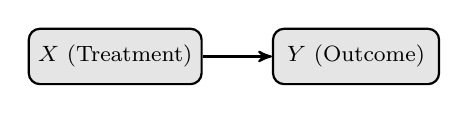
\begin{tikzpicture}[->,shorten >=0pt,shorten <=0pt,node distance=2.5em,thick,node/.style={observedrect},lt/.style={latent}]
\node[node](2){$X \text{ (Treatment)}$};
\node[node, right=of 2](3){$Y \text{ (Outcome)}$};
\path[]
	(2) edge (3);
\end{tikzpicture}
\caption{Causal Bayesian network for example \ref{exm:ranomized_experiment}}
\label{fig:causal_network_example}
\end{figure}



In example \ref{exm:adjusting} we are interested in $\P{Y|do(X=1)}$, the expected high-school graduation rate if we introduce universal preschool. We could compare it to outlawing preschool $\P{Y|do(X=0)}$ or the current status quo $\P{Y}$. It seems reasonable to assume that preschool attendance affects the likelihood of high school graduation \footnote{The effect does not have to be homogeneous, it may depend non-linearly on characteristics of the child, family and school.} and that parental socio-economic status would affect \emph{both} the likelihood of preschool attendance and high school graduation. If we assume that socio-economic status is the only such variable (nothing else affects both attendance \emph{and} graduation), we can represent this problem with the causal Bayesian network in figure \ref{fig:causal_adjust}. In this case, the interventional distribution is not equivalent to the observational one. If parents with high socio-economic status are more likely to send their children to preschool and these children are more likely to graduate high school regardless, comparing the graduation rates of those who attended preschool with those who did not will overstate the benefit of preschool. To obtain the interventional distribution we have to estimate the impact of preschool on high school graduation for each socio-economic level separately and then weight the results by the proportion of the population in that group,

\eqn{
\label{eqn:backdoor_example}
\P{Y|do(X=1)} = \sum_{z \in Z}\P{Y|X=1,Z}\P{Z}
} 

We have seen from these two examples that the expression to estimate the causal effect of an intervention depends on the structure of the causal graph. There is a very powerful and general set of rules that specifies how we can transform observational distributions into interventional ones for a given graph structure. These rules are referred to as the Do-calculus \citep{Pearl2000}. We discuss them further in section \ref{sec:do_calculus}. 


\begin{figure}
\center
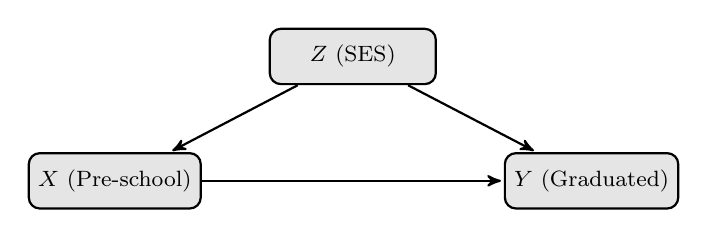
\begin{tikzpicture}[->,>=stealth',shorten >=1pt,auto,node distance=1.2cm, thick,node/.style={observedrect},lt/.style={latent}]

 %nodes
\node[node](1){$Z \text{ (SES)}$};
\node[node, below left=of 1](2){$X \text{ (Pre-school)}$};
\node[node, below right=of 1](3){$Y \text{ (Graduated)}$};
\path[every node/.style={font=\sffamily\small}]
    (1) edge (2) edge (3)
    (2) edge (3); 
\end{tikzpicture}
\caption{Causal Bayesian network for example \ref{exm:adjusting}}
\label{fig:causal_adjust} 
\end{figure}

A causal Bayesian network represents much more information than a Bayesian network with identical structure. A causal network encodes all possible interventions that could be specified with the do-notation. For example, if the network in figure \ref{fig:causal_adjust} were an ordinary Bayesian network and all the variables were binary, the associated distribution could be described by seven parameters. The equivalent causal Bayesian network additionally represents the post-interventional distributions for six possible single variable interventions and twelve possible two variable interventions. Encoding all this information without the assumptions implicit in the causal Bayesian network would require an additional thirty parameters \footnote{After each single variable intervention we have a distribution over two variables, which can be represented by three parameters. After each two variable intervention, we have a distribution over one variables which requires one parameter. This takes us to a total of $6\times3+12\times1 = 30$ additional parameters.}.

Causal Bayesian networks are Bayesian networks, so results that apply to Bayesian networks carry directly across: the local Markov property states that variables are independent of their non-effects given their direct causes. The global Markov property and d-separation also hold in causal networks. D-separation, which characterises which conditional independencies must hold in any distribution that can represented by a given Bayesian network $G$, is key to many important results and algorithms for causal inference. We include a brief review of D-separation in section \ref{sec:dsep}. 


\subsubsection{Limitations of causal Bayesian networks}
A number of criticisms have been levelled at this approach to modelling causality. One is that the definition of an intervention only in terms of setting the value of one or more variables is too precise and that any real world intervention will affect many variables in complex and non-deterministic ways \citep{rickles2009causality,cartwright2007hunting}. However, by augmenting the causal graph with additional variables that model how interventions may take effect, the deterministic do operator can model more complex interventions. For example, in the drug treatment case, we assumed that all subjects complied, taking the treatment or placebo as assigned by the experimenter. But, what if some people failed to take the prescribed treatment? We can model this within the framework of deterministic interventions by adding a node representing what they were prescribed (the intervention) which probabilistically influences the treatment they actually receive (figure \ref{fig:randomized_imperfect_compliance}). Note that the fact that we no longer directly assign the treatment opens the possibility that an unobserved latent variable could affect both the actual treatment taken and the outcome.

\begin{figure}[h]
\centering
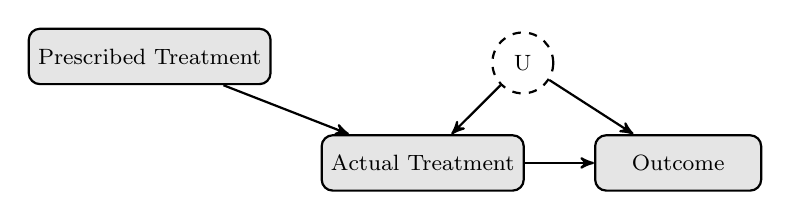
\begin{tikzpicture}[->,shorten >=0pt,shorten <=0pt,node distance=2.5em,thick,node/.style={observedrect},lt/.style={latent}]
\node[node](1){Prescribed Treatment};
\node[node, below right=of 1](2){Actual Treatment};
\node[node, right=of 2](3){Outcome};
\node[lt, above left=of 3](4){U};
\path[]
	(1) edge (2)
	(2) edge (3) 
	(4) edge (3) edge (2);
\end{tikzpicture}
\caption{Randomised treatment with imperfect compliance}
\label{fig:randomized_imperfect_compliance}
\end{figure}

Another key issue with causal Bayesian networks is that they cannot handle cyclic dependencies between variables. Such feedback loops are common in real-life systems, for example the relationship between supply and demand in economics or predator and prey in ecology. We might regard the underlying causal mechanisms in these examples to be acyclic; the number of predators at one time influences the number of prey in the next period and so on. However, if our measurements of these variables must be aggregated over time periods that are longer than the scale at which these interactions occur, the result is a cyclical dependency. Even were we able to measure on shorter timescales, there might then not be sufficient data on each variable for inference. Such problems have mostly been studied within the dynamical systems literature, typically focusing on understanding the stationary or equilibrium state of the system and making very specific assumptions about functional form in order to make problems tractable. \citet{Poole2013} compare the equilibrium approach to reasoning about cyclic problems with structural equation models, which we discuss in section \ref{sec:SEM} and that can be seen as Bayesian causal networks with additional functional assumptions. 

\subsection{Counterfactuals}
\label{sec:counterfactuals}

The Neyman-Rubin model \citep{Rubin1974,Rubin1978,Rosenbaum1983, Rubin2005,Rubin2008} defines causality in terms of potential outcomes, or counterfactuals. Counterfactuals are statements about imagined or alternate realities, are prevalent in everyday language and may play a role in the development of causal reasoning in humans \citep{Weisberg2013}. Causal effects are differences in counterfactual variables: what is the difference between what would have happened if we did one thing versus what would have happened if we did something else. 

In example \ref{exm:ranomized_experiment}, the causal effect of the drug relative to placebo for person $i$ is the difference between what would have happened if they were given the drug, denoted $\cf{y_{i}}{1}$ versus what would have happened if they got the placebo, $\cf{y_{i}}{0}$. The fundamental problem of causal inference is that we can only observe one of these two outcomes, since a given person can only be treated or not treated. The problem can be resolved if, instead of people, there are units that can be assumed to be identical or that will revert exactly to their initial state some time after treatment. This type of assumption often holds to a good approximation in the natural sciences and explains why researchers in these fields are less concerned with causal theory. 

Putting aside any estimates of individual causal effects, it is possible to learn something about the distributions under treatment or placebo. Let $\cf{Y}{1}$ be a random variable representing the potential outcome if treated. The distribution of $\cf{Y}{1}$ is the distribution of $Y$ if everyone was treated. Similarly $Y^{0}$ represents the potential outcome for the placebo. The difference between the probability of recovery, across the population, if everyone was treated and the probability of recovery given placebo is $\P{\cf{Y}{1}}-\P{\cf{Y}{0}}$. We can estimate (from an experimental or observational study):
\begin{itemize}
\item $\P{Y=1|X=1}$, the probability that those who took the treatment will recover
\item $\P{Y=1|X=0}$, the probability that those who were \emph{not} treated will recover
\end{itemize}

Now, for those who took the treatment, the outcome \emph{had} they taken the treatment $\cf{Y}{1}$ is the same as the observed outcome. For those who did not take the treatment, the observed outcome is the same as the outcome \emph{had} they not taken the treatment. Equivalently stated:

\eq{
\P{Y^{0}|X=0}&= \P{Y|X=0}\\
\P{Y^{1}|X=1}&=\P{Y|X=1}
}

If we assume $X \ci Y^{0}$ and $X \ci Y^{1}$:

\eq{
\P{Y^{1}} &= \P{Y^{1}|X=1} = \P{Y|X=1} \\
\P{Y^{0}} &= \P{Y^{0}|X=0} = \P{Y|X=0}
}

This implies the counterfactual distributions are equivalent to the corresponding conditional distributions and, for a binary outcome $Y$, the causal effect is,

\eq{
\P{Y^{1}}-\P{Y^{0}} = \P{Y|X=1} - \P{Y|X=0}
}

The assumptions $X \ci Y^{1}$ and $X \ci Y^{0}$  are referred to as ignorability assumptions \citep{Rosenbaum1983}. They state that the treatment each person receives is independent of whether they would recover if treated and if they would recover if not treated. This is justified in example \ref{exm:ranomized_experiment} due to the randomisation of treatment assignment. In general the treatment assignment will not be independent of the potential outcomes. In example \ref{exm:adjusting}, the children who attended preschool may be more likely to have graduated high school had they in fact not attended than the children who actually did not attend, i.e. $X \nci \cf{Y}{0}$. Similarly, had the poorer children who did not attend pre-school attended they might not have done as well as the children who did in fact attend, i.e. $X \nci \cf{Y}{1}$. A more general form of the ignorability assumption is to identify a set of variables $Z$ such that $X \ci Y^{1}|Z$ and $X \ci Y^{0}|Z$. 

\vspace*{.3cm}
\begin{theorem}[Ignorability \citep{Rosenbaum1983, Pearl2000}] If $X \ci Y^{1}|Z$ and $X \ci Y^{0}|Z$,

\eqn{
\label{eqn:counterfactual1}
\P{\cf{Y}{1}} &= \sum_{z \in Z}\P{Y|X=1,Z}\P{Z}  \\
\label{eqn:counterfactual2}
\P{\cf{Y}{0}} &= \sum_{z \in Z}\P{Y|X=0,Z}\P{Z}
}
\end{theorem}

Assuming that within each socio-economic status level, attendance at pre-school is independent of the likelihood of graduating high-school had a person attended, then the average rate of high-school graduation given a universal pre-school program can be computed from equation \ref{eqn:counterfactual1}. Note, that this agrees with the weighted adjustment formula in equation \ref{eqn:backdoor_example}. 

Another assumption introduced within the Neyman-Rubin causal framework is the Stable Unit Treatment Value Assumption (SUTVA) \citep{Rubin1978}. This is the assumption that the potential outcome for one individual (or unit) does not depend on the treatment assigned to another individual. As an example of a SUTVA violation, suppose disadvantaged four year olds were randomly assigned to attend pre-school. The subsequent school results of children in the control group, who did not attend, could be boosted by the improved behaviour of those who did and who now share the classroom with them. SUTVA violations would manifest as a form of model misspecification in causal Bayesian networks. 

There are objections to counterfactuals arising from the way they describe alternate universes that were never realised. In particular, statements involving joint distributions over counterfactual variables may not be able to be validated empirically \citet{Dawid2000}. One way of looking at counterfactuals is as a natural language short hand for describing highly specific interventions like those denoted by the do-notation. Rather than talking about the distribution of $Y$ given we intervene to set $X=x$ and hold everything else about the system constant we just say what would the distribution of $Y$ be had $X$ been $x$. This is certainly convenient, if rather imprecise. However, the ease with which we can make statements with counterfactuals that cannot be tested with empirical data warrants careful attention. It is important to be clear what assumptions are being made and whether or not they could be validated (at least in theory). 

\subsection{Structural Equation models}
\label{sec:SEM}

Structural equation models (SEMs) describe a deterministic world, where some underlying mechanism or function determines the output of any process for a given input. The mechanism (but not the output) is assumed to be independent of what is fed into it. Uncertainties are not inherent but arise from unmeasured variables. Linear structural equation models have a long history for causal estimation \cite {Wright1921,Haavelmo1943}. More recently, they have been formalised, generalised to the non-linear setting and connected to developments in graphical models to provide a powerful causal framework \citep{Pearl2000}.

Mathematically, each variable is a deterministic function of its direct causes and a noise term that captures unmeasured variables. The noise terms are required to be mutually independent. If there is the possibility that an unmeasured variable influences more than one variable of interest in a study, it must be modelled explicitly as a latent variable. Structural equation models can be represented visually as a network. Each variable is a node and arrows are drawn from causes to their effects. Figure \ref{fig:sem_randomized_treatment} illustrates the SEM for example \ref{exm:ranomized_experiment}.

\begin{figure}[h]
\centering
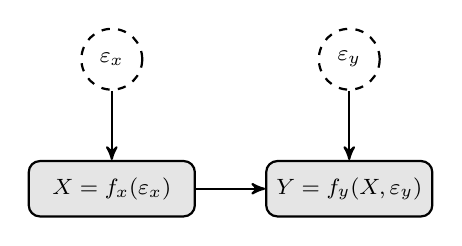
\begin{tikzpicture}[->,shorten >=0pt,shorten <=0pt,node distance=2.5em,thick,node/.style={observedrect},lt/.style={latent}]
\node[node](2){$X = f_x(\epsilon_x)$};
\node[node, right=of 2](3){$Y = f_y(X,\epsilon_y)$};
\node[lt, above=of 3](4){$\epsilon_y$};
\node[lt, above=of 2](5){$\epsilon_x$};
\path[]
	(2) edge (3)
	(4) edge (3)
	(5) edge (2);
\end{tikzpicture}
\caption{SEM for example \ref{exm:ranomized_experiment}}
\label{fig:sem_randomized_treatment}
\end{figure}

This model encodes the assumption that the outcome $y_{i}$ for an individual $i$ is caused solely by the treatment $x_{i}$ they receive and other factors $\epsilon_{y_{i}}$ that are independent of $X$. This is justifiable on the grounds that $X$ is random. The outcome of a coin flip for each patient should not be related to any of their characteristics (hidden or otherwise). Note that the causal graph in figure \ref{fig:sem_randomized_treatment} is identical to that of the Bayesian network for the same problem (figure \ref{fig:causal_network_example}). The latent variables $\epsilon_x$ and $\epsilon_y$ are not explicitly drawn in figure \ref{fig:causal_network_example} as they are captured by the probabilistic nature of the nodes in a Bayesian network.

Taking the \emph{action} $X=1$ corresponds to replacing the equation $X=f_x(\epsilon_x)$ with $X=1$. The function $f_y$ and distribution over $\epsilon_y$ does not change. This results in the interventional distribution, \footnote{We have assumed the variables are discrete only for notational convenience}

\eqn {
\P{Y=y|do(X=1)} = \sum_{\epsilon_y}\P{\epsilon_y}\ind{f_y(1,\epsilon_y)=y}
}

The observational distribution of $Y$ given $X$ is,

\eqn{
\P{Y=y|X=1} &= \sum_{\epsilon_x}\sum_{\epsilon_y}\P{\epsilon_x|X=1}\P{\epsilon_y|\epsilon_x}\ind{f_y(1,\epsilon_y)=y} \\
& = \sum_{\epsilon_y}\P{\epsilon_y}\ind{f_y(1,\epsilon_y)=y} \text{, as } \epsilon_x \ci \epsilon_y
}

The interventional distribution is the same as the observational one. The same argument applies to the intervention $do(X=0)$, and so the causal effect is simply the difference in observed outcomes as found via the causal Bayesian network and counterfactual approaches. 

The SEM for example \ref{exm:adjusting} is shown in figure \ref{fig:sem:preschool}. Intervening to send all children to pre-school replaces the equation $X = f_x(Z,\epsilon_x)$ with $X=1$, leaving all the other functions and distributions in the model unchanged. 

\eqn{
\P{Y=y|do(X=1)} &= \sum_{z}\sum_{\epsilon_y}\P{z}\P{\epsilon_y}\ind{f_y(1,z,\epsilon_y)=y} \\
\label{eqn:sem:adjusting}
&=\sum_{z}\P{z}\underbrace{\sum_{\epsilon_y}\P{\epsilon_y}\ind{f_y(1,z,\epsilon_y)=y}}_{\P{Y=y|X=1,Z=z}}
}
Equation \ref{eqn:sem:adjusting} corresponds to equations \ref{eqn:backdoor_example} and \ref{eqn:counterfactual1}. It is not equivalent to the observational distribution given by:

\eqn{
\P{Y=y|X=1} = \sum_{z}\sum_{\epsilon_y}\P{z|X=1}\P{\epsilon_y}\ind{f_y(1,z,\epsilon_y)=y}
}


\begin{figure}[h]
\centering
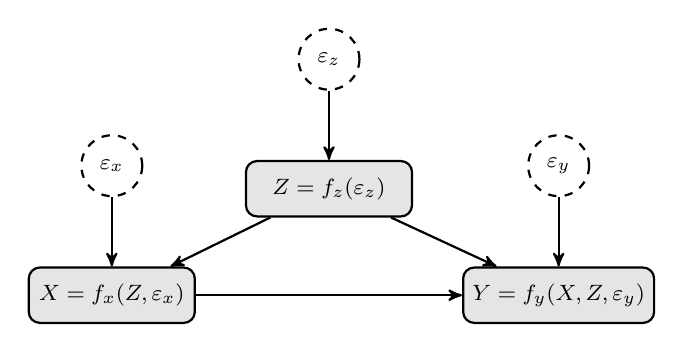
\begin{tikzpicture}[->,shorten >=0pt,shorten <=0pt,node distance=2.5em,thick,node/.style={observedrect},lt/.style={latent}]
\node[node](2){$X = f_x(Z,\epsilon_x)$};
\node[node,above right=of 2](6){$Z = f_z(\epsilon_z)$};
\node[lt, above=of 6](7){$\epsilon_z$};
\node[node, below right=of 6](3){$Y = f_y(X,Z,\epsilon_y)$};
\node[lt, above=of 3](4){$\epsilon_y$};
\node[lt, above=of 2](5){$\epsilon_x$};
\path[]
	(2) edge (3)
	(4) edge (3)
	(5) edge (2)
	(7) edge (6)
	(6) edge (2) edge (3);
\end{tikzpicture}
\caption{SEM for example \ref{exm:adjusting}}
\label{fig:sem:preschool}
\end{figure}

Structural equation models are generally applied with strong constraints on the functional form of the relationship between the variables and noise, which is typically assumed to be additive, $X_i = f_i(\cdot)+\epsilon_i$. A structural equation model with $N$ variables resembles a set of $N$ simultaneous equations, with each variable playing the role of the dependent (left hand side) variable in one equation. However a SEM is, by definition, more than a set of simultaneous equations. By declaring it to be structural, we are saying that it represents \emph{causal} assumptions about the relationships between variables. When visualised as a network, the absence of an arrow between two variables encodes the assumption that one does not cause the other. The similarity between the notation used to describe and analyse structural equation models and simultaneous equations, combined with a reluctance to make explicit statements about causality, has led to some confusion in the interpretation of SEMs \citep{heckman2015causal,Pearl2000}. 

\subsection{Comparing and unifying the models}
\label{sec:unifying_causal_models}

Clarify Cheng's Questions - is there a mechanical method to go from one framework to another, does it matter if variables are discrete or continuous. \todo{}



Remarkably for models developed relatively independently in fields with very different approaches and problems, the models we have discussed can be nicely unified for interventional queries (those that can be expressed with the do-notation). If the network for a structural equation model is acyclic, that is if starting from any node and following edges in the direction of the arrows you cannot return to the starting point, then it implies a recursive factorisation of the joint distribution over its variables. In other words, the network is a causal Bayesian network. All of the results that apply to causal Bayesian networks also apply to acyclic structural equation models.  Taking an action that sets a variable to a specific value equates to replacing the equation for that variable with a constant. This corresponds to dropping a term in the factorisation and the truncated product formula (equation \ref{eq:truncatedproduct}). Thus, the interventional query $P(Y|do(X))$ is identical in these two frameworks. We can also connect this to counterfactuals via:

\begin{equation}
\begin{aligned}
&Y^{0} \equiv P(Y|do(X=0)) \\
&Y^{1} \equiv P(Y|do(X=1))
\end{aligned}
\end{equation}

The assumption $\epsilon_{X} \ci \epsilon_{Y}$, stated for our structural equation model, translates to $X \ci (Y^{0},Y^{1})$ in the language of counterfactuals. When discussing the counterfactual model, we made the slightly weaker assumption:

\begin{equation}
\label{eq:weakignore}
X \ci Y^{0} \text{ and } X \ci Y^{1}
\end{equation}

It is possible to relax the independence of errors assumption for SEMs to correspond exactly with the form of equation (\ref{eq:weakignore}) without losing any of the power provided by d-separation and graphical identification rules \citep{Richardson2013}. The correspondence between the models for interventional queries (those that can be phrased using the do-notation) makes it straightforward to combine key results and algorithms developed within any of these frameworks. For example, you can draw a causal graphical network to determine if a problem is identifiable and which variables should be adjusted for to obtain an unbiased causal estimate. Then use propensity scores \citep{Rosenbaum1983} to estimate the effect. If non-parametric assumptions are insufficient for identification or lead to overly large uncertainties, you can specify additional assumptions by phrasing your model in terms of structural equations. The frameworks do differ when it comes to causal queries that involve joint or nested counterfactuals and cannot be expressed with the do-notation. These types of queries arise in the study of mediation \citep{Pearl2014,Imai2010a,VanderWeele2011} and in legal decisions, particularly on issues such as discrimination \citep{Pearl2000}. 

In practice, differences in focus and approach between the fields in which each model dominates eclipse the actual differences in the frameworks. The work on causal graphical models \citep{Pearl2000,Sprites2000} focuses on asymptotic, non-parametric estimation and rigorous theoretical foundations. The Neyman-Rubin framework builds on the understanding of randomised experiments and generalises to quasi-experimental and observational settings, with a particular focus on non-random assignment to treatment. This research emphasises estimation of average causal effects and provides practical methods for estimation, in particular, propensity scores; a method to control for multiple variables in high dimensional settings with finite data \citep{Rosenbaum1983}. In economics, inferring causal effects from non-experimental data to support policy decisions is central to the field. Economists are often interested in more informative measures of the distribution of causal effects than the mean and make extensive use of structural equation models, generally with strong parametric assumptions \citep{Heckman2008}. In addition, the parametric structural equation models favoured in economics can be extended to analyse cyclic (otherwise referred to as non-recursive) models. 

\subsection{What does a causal model give us? Resolving Simpson's paradox}

We will now demonstrate our new notation and frameworks for causal inference to resolve a fascinating paradox noted by \citet{yule1903notes}, demonstrated in real data by \citet{Cohen1934}, and popularised by \citet{simpson1951interpretation}. The following example is adapted from \citet{Pearl2000}. Suppose a doctor has two treatments, A and B, which she offers to patients to prevent heart disease. She keeps track of the medication her patients choose and whether or not the treatment is successful. She obtains the results in table \ref{tab:simpson1}.

\begin{table}[h]
\caption{Treatment results}
\label{tab:simpson1}
\center
\begin{tabular}{c c c c c}
Treatment & Success & Fail & Total & Success Rate\\
\hline
\rowcolor[gray]{0.9} 
A &  87 & 13 & 100 & 87\%\\
\rowcolor{white} B & 75 & 25 & 100 & 75\%\\
\hline
\end{tabular}
\end{table}

Drug A appears to perform better. However, having read the latest literature on how medications affect men and women differently, she decides to break down her results by gender to see how well the drugs perform for each group, and obtains the data in table \ref{tab:simpson2}.

\begin{table}[h]
\caption{Treatment results by gender}
\label{tab:simpson2}
\center
\begin{tabular}{c c c c c c}
Gender & Treatment & Success & Fail & Total & Success Rate\\
\hline
\rowcolor[gray]{0.9}
M & A & 12 & 8 & 20 & 60\%\\
M & B & 56 & 24 & 80 & 70\%\\
\rowcolor[gray]{0.9}
F & A & 75 & 5 & 80 & 94\%\\
F & B & 19 & 1 & 20 & 95\%\\
\hline
\end{tabular}
\end{table}

Once the data is broken down by gender, drug B looks better for both men \emph{and} women. Suppose the doctor must choose only one drug to prescribe to all her patients in future (perhaps she must recommend which to subsidise under a national health scheme). Should she choose A or B? The ambiguity in this question lies at the heart of Simpson's paradox. How does causal modelling resolve the paradox? The key is that the doctor is trying to choose between \emph{interventions}. She wants to know what the success rate will be if she changes her practice to give all the patients one drug, rather than allowing them to choose as currently occurs. 

Let's represent the treatment by the variable $T$, the gender of the patient by $Z$ and whether or not the treatment was successful by $Y$. The doctor is concerned with $\P{Y|do(T)}$, not the standard conditional distributions $\P{Y|T}$. Unfortunately, the data in tables \ref{tab:simpson1} and \ref{tab:simpson2} is insufficient to enable estimation of the interventional distribution $\P{Y|do(T)}$ or determine if $do(T=A)$ is better or worse than $do(T=B)$. Some assumptions about the causal relationships between the variables are required. In this example, it seems reasonable to conclude that gender may affect the treatment chosen and the outcome. Assuming there are no other such confounding variables (for example income) then we obtain the causal network in figure \ref{fig:simpsons_paradox}.

\begin{figure}[h]
\centering
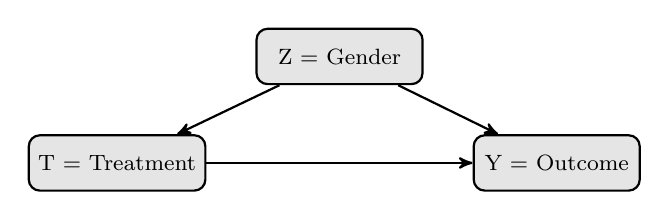
\begin{tikzpicture}[->,shorten >=0pt,shorten <=0pt,node distance=2.5em,thick,node/.style={observedrect},lt/.style={latent}]
\node[node](1){Z = Gender};
\node[node, below left=of 1](2){T = Treatment};
\node[node, below right=of 1](3){Y = Outcome};
\path[]
	(1) edge (2) edge (3) 
	(2) edge (3);
\end{tikzpicture}
\caption{An example of causal network that can give rise to Simpson's Paradox. In this case, we should select treatment on the basis of the gender-specific results.}
\label{fig:simpsons_paradox}
\end{figure}

With this model, women are more likely to choose drug A and are also more likely to recover than men, regardless of the treatment they receive. Knowing a patient took drug A indicates they are more likely to be female. When we compare the group of people who took A against those who took B, the effect of the higher proportion of females in the first group conceals the greater benefit of drug B, leading to an apparent reversal in effectiveness. However, when the doctor intervenes to set the treatment each person receives, there will no longer be a link from gender to treatment. So, in this case she should choose the drug to prescribe from the gender-specific table (and weight by the proportion of the population that belongs to each gender). Drug B is the better choice.

\eqn{
\P{Y|do(T)} = \P{Y|T,female}\P{female}+ \P{Y|T,male}\P{male}
}

Is the solution to Simpson's paradox to always to break down the data by as many variables as possible? No. Suppose we have the identical data as in \ref{tab:simpson1} and \ref{tab:simpson2}, but replace the column name 'gender' with 'blood pressure', 'M' with 'high' and 'F' with 'normal'. This is a drug designed to prevent heart disease. One pathway to doing so might well be to lower blood pressure. Figure \ref{fig:simpsons_paradox2} shows a plausible causal graph for this setting. It differs from the graph in figure \ref{fig:simpsons_paradox} only in the direction of a single link. Now, however, table \ref{tab:simpson2} tells us that people who took treatment $A$ had better blood pressure control and better overall outcomes. In this setting $\P{Y|do(T)} = \P{Y|T}$ and drug A is the better choice. 

\begin{figure}[h]
\centering
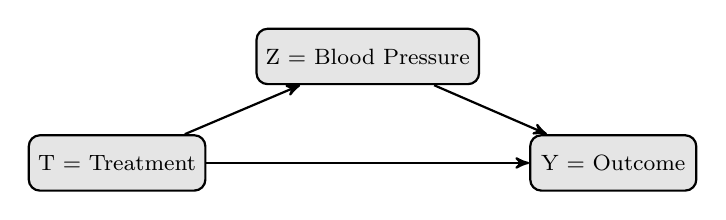
\begin{tikzpicture}[->,shorten >=0pt,shorten <=0pt,node distance=2.5em,thick,node/.style={observedrect},lt/.style={latent}]
\node[node](1){Z = Blood Pressure};
\node[node, below left=of 1](2){T = Treatment};
\node[node, below right=of 1](3){Y = Outcome};
\path[]
	(1) edge (3) 
	(2) edge (3)
	(2) edge (1);
\end{tikzpicture}
\caption{Another causal network that can exhibit Simpson's paradox. In this case, \quotes{the solution} is not to stratify on $Z$.}
\label{fig:simpsons_paradox2}
\end{figure}

Note that we have not changed the data itself, only the description of the variables that it is associated with. This illustrates that the resolution to Simpson's paradox lies fundamentally not in the data, but in the assumptions we are willing to make. From a purely statistical viewpoint, there is no paradox. The reversal just stems from the mathematical property of ratios expressed in equation \ref{eqn:simpsons_paradox} and represented graphically in figure \ref{fig:simpsons_vector}. The paradox only arises when we attempt to use the data to select an intervention and is resolved when we apply a causal approach to do so.

\eqn{
\label{eqn:simpsons_paradox}
\exists \set{N_1,...N_4, N_1'...N_4'} \in \mathbb{N} : \; 
\textcolor{green}{\frac{N_1}{N_2}< \frac{N_1'}{N_2'}}, \;\; 
\textcolor{blue}{ \frac{N_3}{N_4}<\frac{N_3'}{N_4'}}
 \text{ and } \frac{N_1+N_3}{N_2+N_4} > \frac{N_1'+N_3'}{N_2'+N_4'}
}

\begin{figure}
\centering
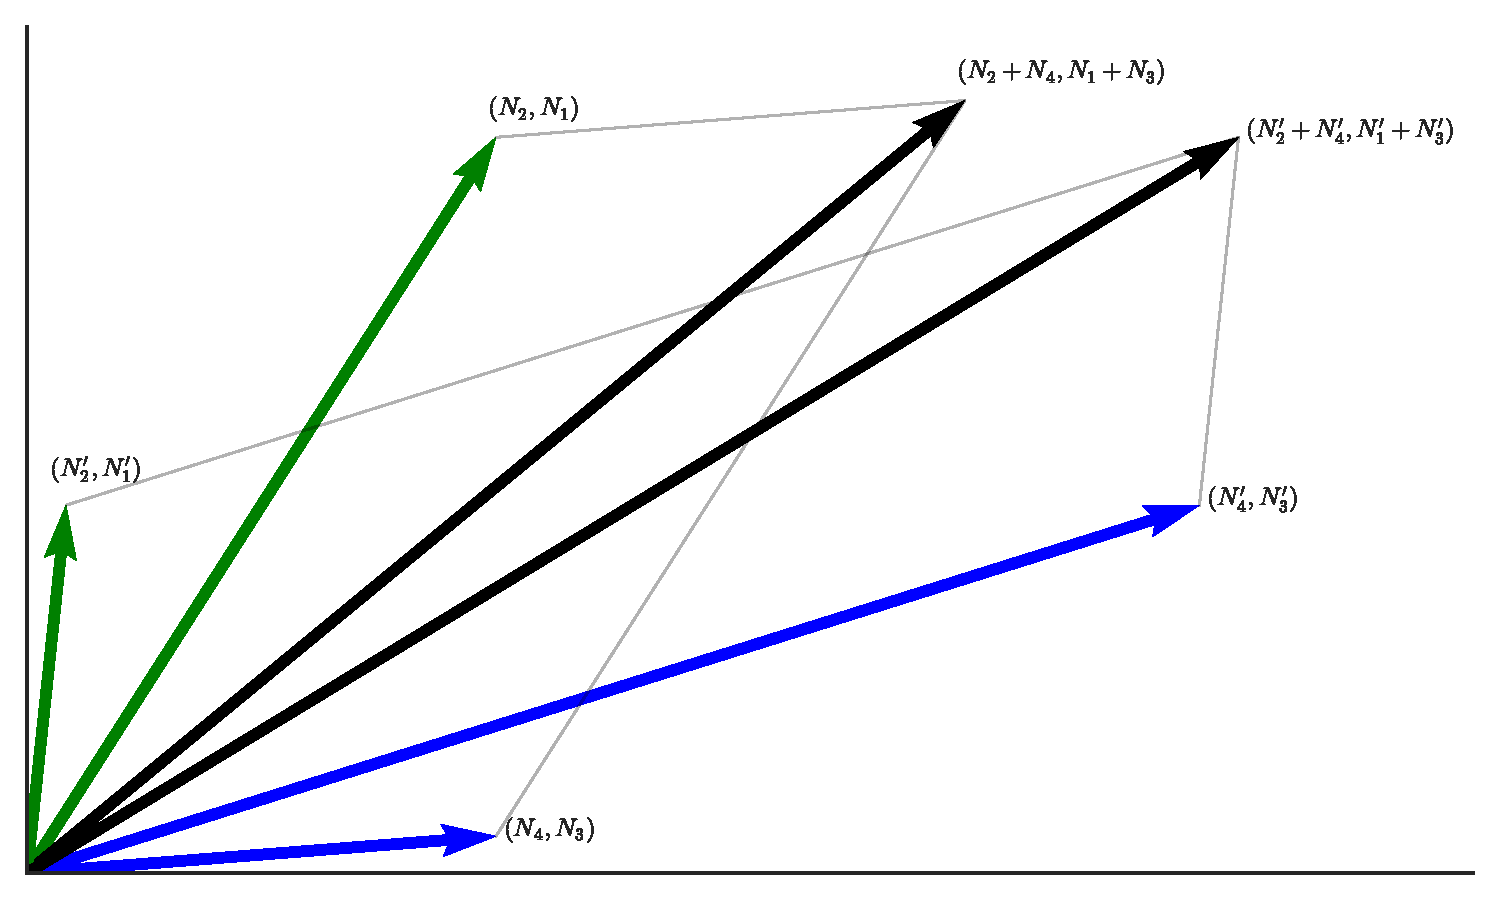
\includegraphics[scale=.4]{figures/simpson_vector}
\caption{Simpson's reversal visualised. The ratios involving $N_i'$ are steeper than those involving $N_i$ for both the blue and green vectors. However, when we sum them, the ratio is steeper for the un-primed variables.}
\label{fig:simpsons_vector}
\end{figure}

There are many other plausible causal graphs for both scenarios above. Perhaps income affects drug choice as well as gender, or gender might affect treatment choice and blood pressure control given treatment, etc. Causal modelling provides a powerful tool to specify such assumptions and to determine how to estimate causal effects for a given model as we discuss in the next section.

\section{Answering Causal Questions} 
\label{sec:causal effect estimation}
We can roughly categorise the problems studied within causal inference from observational data into two groups, causal effect estimation and causal discovery. In causal effect estimation we assume (at least implicitly) that key aspects of the causal graph are known. The goal is then to estimate the effect of an intervention or range of interventions in the system. Causal effect estimation is implicit in countless studies in economics, social science and epidemiology of everything from the effect of education on earnings \citep{card1999causal}, diet on cancer \citep{bingham2004diet} and breastfeeding on intelligence \citep{jain2002good} to the effect of pet ownership on survival after a heart attack \citep{friedmann1995pet}. Almost every time someone runs a regression model the key quantity of interest is a causal effect. Given how it underlies so much of our scientific progress, there is a enormous potential in properly understanding when we can draw causal conclusions, the assumptions required to do so, and how to best leverage those assumptions to infer as much information as possible from the available data. 

Causal discovery aims to leverage much broader assumptions to learn the structure of causal graphs from data. This is critical in fields where there is abundant data, but limited theoretical knowledge on how variables are related to one another. Causal discovery algorithms are being applied in bioinformatics \citep{Bay2002,Sachs2005,Ram2006,Alekseyenko2011,Statnikov2012,Gao2015,Sokolova2015,Taruttis2015}, medical imaging \citep{Ramsey2010} and climate science \citep{Uphoff2013}. An effective and generalisable approach for causal discovery would be a major step towards the automation of the scientific endeavour. In this thesis, I have focused on problems where the structure of the causal graph is known. Extending my work to problems where the causal structure is unknown, leveraging the work on causal discovery, is a rich and fascinating line of potential future work, which I discuss briefly in section \ref{sec:causal_bandit_discussion}. 

\subsection{Mapping from observational to interventional distributions}

A central component of estimating causal effects from observational data is determining if and how we can write expressions for the interventional distributions of interest in terms of observational quantities, which can be measured. We did this on an ad-hoc basis to resolve the examples discussed in section \ref{sec:causal_models}. In this section we describe a principled approach to mapping observational quantities to interventional ones and then, in section \ref{sec:causal_effect_under_ignorability}, discuss the key issues involved in estimating such expressions from finite sample data. We assume the basic structure of the graph is known. That is, we assume that we can draw a network containing (at a minimum):

\begin{itemize}
\item the target/outcome variable we care about,
\item the focus/treatment variables on which we are considering interventions,
\item any variables which act to confound two or more of the other variables we have included, and
\item any links between variables we have included. 
\end{itemize}

Some of these variables may be latent, in that the available data does not record their value, however their position in the network is assumed to be known. For example, consider estimating the impact of schooling on wages. Some measure of inherent ability could influence both the number of years of schooling people choose to pursue and the wages they receive. Even if we have no data to directly assess people's inherent ability we must include ability in the graph because it influences two of the variables we are modelling. 

How can the structure of the causal graph be leveraged to compute interventional distributions from observational ones? Given the graph corresponding to the observational distribution, the graph after any intervention can be obtained by removing any links into variables directly set by the intervention. The joint interventional distribution is the product of the factors associated with the interventional graph, as given by the truncated product formula \ref{eq:truncatedproduct}. If there are no latent variables the interventional distribution of interest can be obtained by marginalising over the joint (interventional) distribution. However, if there are latent variables, the joint interventional distribution will contain terms that cannot be estimated from the observed data. 

The key to estimating causal effects in the presence of latent variables lies in combining the assumption of how an intervention changes the graph, encoded by the truncated product formula, with information the graph structure provides about conditional independencies between variables. 
By leveraging conditional independencies, we can effectively localise the effect of an intervention to a specific part of a larger graph. This gives rise to the do-calculus \citep{Pearl2000}. The do calculus consists of three rules. They are derived from the causal information encoded in a causal network and the properties of d-separation and do not require any additional assumptions other than that of specifying the causal network.

\subsubsection{Independence in Bayesian networks: D-separation}
\label{sec:dsep}

Many causal algorithms are based on leveraging the independence properties encoded in Bayesian networks. Therefore, in this section, we briefly review the key properties of Bayesian networks. A more thorough introduction (including proofs) can be found in \citep{Koller2009}. Recall that a Bayesian network is a way of representing the joint distribution over its variables in a way that highlights conditional independencies between them. 

\vspace{.3cm}
\begin{theorem}
\textbf{(Local Markov condition)} Given a Bayesian network $G$ with nodes $X_{1}...X_{N}$, each variable $X_{i}$ is independent of its non-decedents given its parents in $G$ for all distributions $P(X_{1}...X_{N})$ that are compatible with $G$.
\end{theorem}

The set of conditional independence relations given by the local Markov condition can enforce additional independencies that also hold in all distributions that are compatible with $G$. D-separation is an algorithm that extends the local Markov property to find these additional independencies. It provides a simple way of reading from a network if a given conditional independence statement is true in all distributions compatible with that network.

The statement that $X$ is conditionally independent of $Y$ given $Z$ implies that if we know $Z$, learning the value of $Y$ provides no additional information about $X$. From a graphical perspective, you can think of this as $Z$ blocks the flow of information from $X$ to $Y$ in the network. Figure \ref{fig:dseptriples} shows all possible network paths from a variable $X$ to $Y$ via $Z$. In figures (a) to (c) the path is blocked if we condition on $Z$ and unblocked otherwise. In figure (d), the path is unblocked if we condition on $Z$ and blocked otherwise. 

The structure in figure \ref{fig:dseptripple4} is referred to as a collider or v-structure. The counter-intuitive result that conditioning on $Z$ introduces dependence between $X$ and $Y$ is called the \textit{explaining away phenomena}. As an example, consider a scholarship available to female or disadvantaged students. Let $X$ be gender, $Y$ be family background and $Z$ receipt of the scholarship. There are roughly equal numbers of boys and girls in both poor and wealthy families so $X$ and $Y$ are independent. However, if we know a student is receiving a scholarship, then learning that they are male  increases the probability that they are disadvantaged.
\begin{figure}[h]
\centering
\begin{subfigure}[t]{0.2\textwidth}
\centering
\caption{$X \ci Y| Z$}
\label{fig:dseptripple1}
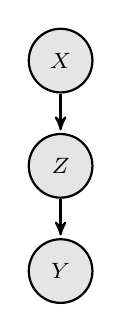
\begin{tikzpicture}[->,>=stealth',shorten >=1pt,auto,node distance=.5cm,
  thick,main node/.style={observed}]
\node[main node](1){$X$};
\node[main node, below =of 1](2){$Z$};
\node[main node, below =of 2](3){$Y$};
 \path[every node/.style={font=\sffamily\small}]
    (1) edge node {} (2)
    (2) edge node {} (3);	
\end{tikzpicture}
\end{subfigure}
\begin{subfigure}[t]{0.2\textwidth}
\centering
\caption{$X \ci Y|Z$}
\label{fig:dseptripple2}
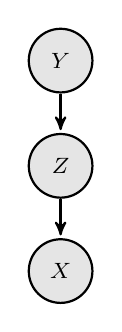
\begin{tikzpicture}[->,>=stealth',shorten >=1pt,auto,node distance=.5cm,
  thick,main node/.style={observed}]
\node[main node](1){$Y$};
\node[main node, below =of 1](2){$Z$};
\node[main node, below =of 2](3){$X$};
 \path[every node/.style={font=\sffamily\small}]
    (1) edge node {} (2)
    (2) edge node {} (3);	
\end{tikzpicture}
\end{subfigure}
\begin{subfigure}[t]{0.2\textwidth}
\centering
\caption{$X \ci Y|Z$}
\label{fig:dseptripple3}
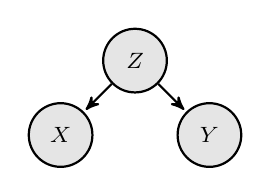
\begin{tikzpicture}[->,>=stealth',shorten >=1pt,auto,node distance=.5cm,
  thick,main node/.style={observed}]
\node[main node](1){$Z$};
\node[main node, below left =of 1](2){$X$};
\node[main node, below right=of 1](3){$Y$};
 \path[every node/.style={font=\sffamily\small}]
    (1) edge node {} (2)
        edge node {} (3);	
\end{tikzpicture}
\end{subfigure}
\begin{subfigure}[t]{0.2\textwidth}
\centering
\caption{$X \ci Y|\{\}$}
\label{fig:dseptripple4}
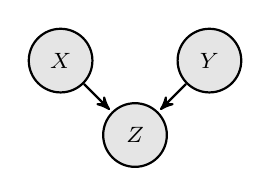
\begin{tikzpicture}[->,>=stealth',shorten >=1pt,auto,node distance=.5cm,
  thick,main node/.style={observed}]
\node[main node](1){$Z$};
\node[main node, above left =of 1](2){$X$};
\node[main node, above right =of 1](3){$Y$};
 \path[every node/.style={font=\sffamily\small}]
    (2) edge node {} (1)
    (3) edge node {} (1);	
\end{tikzpicture}
\end{subfigure}
\caption{All possible two edge paths from $X$ to $Y$ via $Z$}
\label{fig:dseptriples}
\end{figure}

\vspace{.3cm}
\begin{definition}[unblocked path]
\label{def:unblocked}
A path from $X$ to $Y$ is a sequence of edges linking adjacent nodes starting at $X$ and finishing at $Y$,  $(X,V_{1},V_{2}...V_{k},Y)$. It is unblocked if every triple, $X-V_{1}-V_{2},V_{1}-V_{2}-V{3},...,V_{k-1}-V_{k}-Y$ in the path is unblocked (each triple will belong to one of the cases in figure \ref{fig:dseptriples})
\end{definition}

\vspace{.3cm}
\begin{definition}[d-separation]
\label{def:dsep}
The variables $\boldsymbol{X}$ are d-separated from $\boldsymbol{Y}$ given $\boldsymbol{Z}$ in the network $G$ if, there are no unblocked paths from any $X \in \boldsymbol{X}$ to any $Y \in \boldsymbol{Y}$ after conditioning on $\boldsymbol{Z}$. 
\end{definition}

\vspace{.3cm}
\begin{theorem}[d-separation and conditional independence]
\label{thrm:dsep_independence}
If a set of variables $\boldsymbol{Z}$ d-separates $\boldsymbol{X}$ and $\boldsymbol{Y}$ in a Bayesian network $G$ then ${(\boldsymbol{X} \ci \boldsymbol{Y}|\boldsymbol{Z})}$ in all distributions $P$ compatible with $G$. Conversely, if $\boldsymbol{X}$ and $\boldsymbol{Y}$ are d-connected (not d-separated) given $\boldsymbol{Z}$ then it is possible to construct a distribution $P'$ that factorises over $G$ in which they are dependent. 
\end{theorem}

Theorem \ref{thrm:dsep_independence} says that independencies implied by d-separation on a graph hold in every distribution that can be factored over that graph and that if ${(\boldsymbol{X} \ci \boldsymbol{Y}|\boldsymbol{Z})}$ in \emph{all} distributions that can be factored over $G$ then they are d-separated in $G$. If we denote the independencies implied by d-separation in a graph by $\indep{G}$ and the set of independencies in a distribution by $\indep{P}$ then $\indep{G} \subseteq \indep{P}$. 

If $\indep{G} = \indep{P}$ then $G$ is called a perfect map for $P$. However, it is possible to construct distributions that do not have a perfect map; that is, they contain conditional independencies that cannot be represented by d-separation. The presence of deterministic relationships between variables is one instance where this occurs. If there is a Bayesian network $G$ with some deterministic nodes, then we cannot conclude that if $X$ and $Y$ are d-connected then there exists a distribution $P'$ \emph{consistent} with $G$ in which they are dependent. This does not conflict with theorem \ref{thrm:dsep_independence}, as \emph{consistent} in this setting requires that $P'$ both factorises over $G$ and satisfies the specified the deterministic relations between variables. This subtlety led to confusion in the independencies that hold between counterfactuals via twin networks \citep{Pearl2000,Richardson2013} and demonstrates the caution required in using d-connectedness to assert lack of independence. D-separation can be extended to compute the additional independencies implied by a graph in which certain nodes are known to be deterministic \citep{Geiger1990}. 

\subsubsection{The Do Calculus} 
\label{sec:do_calculus}

The do-calculus is a set of three rules \citep{Pearl1995} that can be applied to simplify the expression for an interventional distribution. If by repeated application of the do-calculus, along with standard probability transformations, we can obtain an expression containing only observational quantities then we can use it to estimate the interventional distribution from observational data. Let $\boldsymbol{X}$,$\boldsymbol{Y}$,$\boldsymbol{Z}$ and $\boldsymbol{W}$ be disjoint sets of variables in a causal graph $G$. We denote the graph $G$ after the an intervention $do(\boldsymbol{X})$, which has the effect of removing all edges into variables in $\boldsymbol{X}$, as $G_{\overline{\boldsymbol{X}}}$

\paragraph{Rule 1: (adding or removing evidence)} 

Rule 1 allows us to remove (or insert) observational evidence from the right hand side of a conditional interventional distribution. It follows directly from the fact that the relationship between d-separation in a network and independence in the corresponding probability distribution still applies after an intervention. 


If $(\boldsymbol{Y} \ci \boldsymbol{W} | \boldsymbol{Z},\boldsymbol{X})$ in $G_{\overline{\boldsymbol{X}}}$:
\eqn{
\label{eq:Do1}
 P(\boldsymbol{Y}|do(\boldsymbol{X}=\boldsymbol{x}),\boldsymbol{Z}=\boldsymbol{z},\boldsymbol{W}=\boldsymbol{w}) = P(\boldsymbol{Y}|do(\boldsymbol{X}=\boldsymbol{x}),\boldsymbol{Z}=\boldsymbol{z}) 
}


\begin{figure}[h]
\centering
\begin{subfigure}[t]{0.3\textwidth}
\centering
\caption{original network, $G$}
\label{fig:mutilatedOriginal}
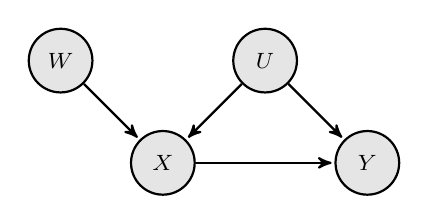
\begin{tikzpicture}[->,>=stealth',shorten >=1pt,auto,node distance=1cm,
  thick,main node/.style={observed}]

 %nodes
\node[main node](1){$U$};
\node[main node, below left=of 1](2){$X$};
\node[main node, below right=of 1](3){$Y$};
\node[main node, above left=of 2](4){$W$};


 \path[every node/.style={font=\sffamily\small}]
    (1) edge node {} (2)
    	edge node {} (3)
    (2) edge node {} (3)
    (4) edge node {} (2);
	
\end{tikzpicture} 
\end{subfigure}
\begin{subfigure}[t]{0.5\textwidth}
\centering
\caption{network after the intervention $do(X=x)$, $G_{\overline{X}}$}
\label{fig:mutilatedAfter}
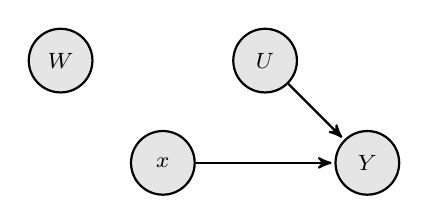
\begin{tikzpicture}[->,>=stealth',shorten >=1pt,auto,node distance=1cm,
  thick,main node/.style={observed}]

 %nodes
\node[main node](1){$U$};
\node[main node, below left=of 1](2){$x$};
\node[main node, below right=of 1](3){$Y$};
\node[main node, above left=of 2](4){$W$};


 \path[every node/.style={font=\sffamily\small}]
    (1) edge node {} (3)
    (2) edge node {} (3);
    
\end{tikzpicture}
\end{subfigure}
\caption{Rule 1 example. $(Y \ci W|X)$ in  $G_{\overline{\boldsymbol{X}}} \implies \P{Y|do(X),W} = \P{Y|do(X)}$ }
\label{fig:mutilatednet}
\end{figure}

\paragraph{Rule 2: (exchanging actions with observations)}
Rule 2 describes when conditioning on $\boldsymbol{X} = \boldsymbol{x}$ and intervening, $do(\boldsymbol{X}=\boldsymbol{x})$, have the same effect on the distribution over $\boldsymbol{Y}$. Let $G_{\underline{\boldsymbol{X}}}$ denote the causal graph $G$ with all edges \emph{leaving} $X$ removed.

If  $(\boldsymbol{Y} \ci \boldsymbol{X}|\boldsymbol{W})$ in $G_{\underline{\boldsymbol{X}}}$:
\eqn{
\label{eq:Do22}
P(\boldsymbol{Y}|do(\boldsymbol{X}=\boldsymbol{x}),\boldsymbol{W}) = P(\boldsymbol{Y}|\boldsymbol{X}=\boldsymbol{x},\boldsymbol{W})
}

The intuition behind this is that interventional distributions differ from observational ones due to the presence of indirect paths between $X$ and $Y$. Observing a variable $X$ provides information about $Y$ both directly and indirectly, by changing our belief about the distribution of the parents of $X$. However, setting $X$ tells us nothing about its parents and therefore affects $Y$ only via direct paths out of $X$. Removing edges \emph{leaving} $X$ removes all the direct paths out of $X$. If $X$ is then independent of $Y$ (conditional on $W$), that indicates there are no indirect paths. This implies conditioning on $X$ is equivalent to setting $X$ (given $W$).

Equation \ref{eq:Do22} does not cover cases where acting on one set of variables allows us to replace acting on another set with conditioning (see figure \ref{fig:rule2_2}). The general form of rule 2 is given in equation \ref{eq:Do2}.

If  $(\boldsymbol{Y} \ci \boldsymbol{X}|\boldsymbol{W},\boldsymbol{Z})$ in $G_{\underline{\boldsymbol{X}}\overline{\boldsymbol{Z}}}$:
\eqn{
\label{eq:Do2}
P(\boldsymbol{Y}|do(\boldsymbol{X}=\boldsymbol{x}),
do(\boldsymbol{Z}=\boldsymbol{z}),
\boldsymbol{W}) = P(\boldsymbol{Y}|\boldsymbol{X}=\boldsymbol{x},do(\boldsymbol{Z}=\boldsymbol{z}),\boldsymbol{W})
}

\begin{figure}[h]
\centering
\begin{subfigure}[t]{0.29\textwidth}
\centering
\caption{original network, $G$}
\label{fig:rule2_orig}
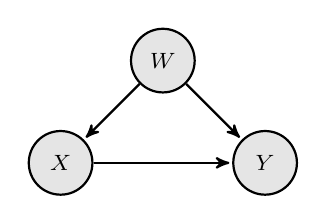
\begin{tikzpicture}[->,>=stealth',shorten >=1pt,auto,node distance=1cm,
  thick,main node/.style={observed}]

 %nodes
\node[main node](1){$W$};
\node[main node, below left=of 1](2){$X$};
\node[main node, below right=of 1](3){$Y$};
 \path[every node/.style={font=\sffamily\small}]
    (1) edge  (2)  edge  (3)
    (2) edge (3);
\end{tikzpicture} 
\end{subfigure}
\begin{subfigure}[t]{0.29\textwidth}
\centering
\caption{$G_{\overline{X}}$}
\label{fig:rule2_after}
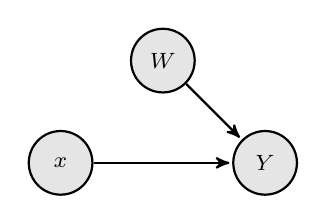
\begin{tikzpicture}[->,>=stealth',shorten >=1pt,auto,node distance=1cm,
  thick,main node/.style={observed}]

 %nodes
\node[main node](1){$W$};
\node[main node, below left=of 1](2){$x$};
\node[main node, below right=of 1](3){$Y$};


 \path[every node/.style={font=\sffamily\small}]
    (1)	edge (3)
    (2) edge (3);
\end{tikzpicture} 
\end{subfigure}
\begin{subfigure}[t]{0.29\textwidth}
\centering
\caption{$G_{\underline{X}}$}
\label{fig:rule2_indirect}
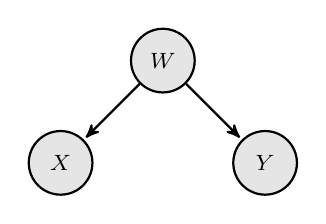
\begin{tikzpicture}[->,>=stealth',shorten >=1pt,auto,node distance=1cm,
  thick,main node/.style={observed}]

 %nodes
\node[main node](1){$W$};
\node[main node, below left=of 1](2){$X$};
\node[main node, below right=of 1](3){$Y$};


 \path[every node/.style={font=\sffamily\small}]
    (1) edge  (2)
    	edge  (3);
    
\end{tikzpicture} 
\end{subfigure}
\caption{An example of rule 2 with a single intervention $(Y \ci X|W)$ in  $G_{\underline{\boldsymbol{X}}} \implies \P{Y|do(X),W} = \P{Y|X,W}$. In this example, observing $X$ provides information about $Y$ both directly and indirectly, because knowing $X$ tells us something about $W$, which also influences $Y$. If we condition on $W$, we block this indirect path.}
\label{fig:rule2}
\end{figure}

\begin{figure}[h]
\centering
\begin{subfigure}[t]{0.29\textwidth}
\centering
\caption{original network, $G$}
\label{fig:rule22_orig}
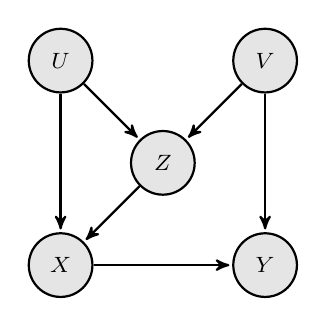
\begin{tikzpicture}[->,>=stealth',shorten >=1pt,auto,node distance=1cm,
  thick,main node/.style={observed}]

 %nodes
\node[main node](1){$Z$};
\node[main node, below left=of 1](2){$X$};
\node[main node, below right=of 1](3){$Y$};
\node[main node, above left=of 1](4){$U$};
\node[main node, above right=of 1](5){$V$};
 \path[every node/.style={font=\sffamily\small}]
    (1) edge  (2)
    (2) edge (3)
    (4) edge (1) edge (2)
    (5) edge (1) edge (3);
\end{tikzpicture} 
\end{subfigure}
\begin{subfigure}[t]{0.29\textwidth}
\centering
\caption{after $do(Z)$, $G_{\overline{Z}}$}
\label{fig:rule22_after}
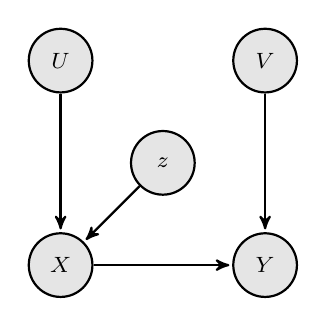
\begin{tikzpicture}[->,>=stealth',shorten >=1pt,auto,node distance=1cm,
  thick,main node/.style={observed}]

 %nodes
\node[main node](1){$z$};
\node[main node, below left=of 1](2){$X$};
\node[main node, below right=of 1](3){$Y$};
\node[main node, above left=of 1](4){$U$};
\node[main node, above right=of 1](5){$V$};
 \path[every node/.style={font=\sffamily\small}]
    (1) edge  (2)
    (2) edge (3)
    (4) edge (2)
    (5) edge (3);
\end{tikzpicture} 
\end{subfigure}
\begin{subfigure}[t]{0.29\textwidth}
\centering
\caption{$G_{\underline{X}\overline{Z}}$}
\label{fig:rule22_indirect}
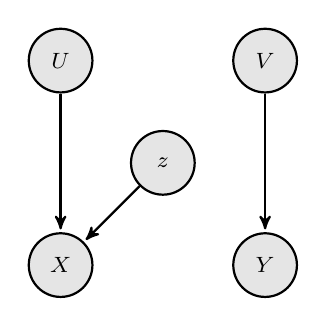
\begin{tikzpicture}[->,>=stealth',shorten >=1pt,auto,node distance=1cm,
  thick,main node/.style={observed}]

 %nodes
\node[main node](1){$z$};
\node[main node, below left=of 1](2){$X$};
\node[main node, below right=of 1](3){$Y$};
\node[main node, above left=of 1](4){$U$};
\node[main node, above right=of 1](5){$V$};
 \path[every node/.style={font=\sffamily\small}]
    (1) edge  (2)
    (4) edge (2)
    (5) edge (3);
\end{tikzpicture} 
\end{subfigure}
\caption{An example of applying equation \ref{eq:Do2}. In this case $(Y \ci X|Z) \text{ in } G_{\underline{X}\overline{Z}}\implies \P{Y|do(X=x),do(Z=z)} = \P{Y|X=x,do(Z=z)}$. Observing, rather than intervening, on $Z$ would not have allowed us to exchange $do(X=x)$ for $X=x$. Conditioning on $Z$ does block the indirect path $X-Z-V-Y$ but opens $X-U-Z-V-Y$.  }
\label{fig:rule2_2}
\end{figure}

\paragraph{Rule 3: (adding or removing actions)}
This rule describes cases where the intervention $do(\boldsymbol{X}=\boldsymbol{x})$ has no effect on the distribution of the outcome $\boldsymbol{Y}$. A simple case of rule 3 is given in equation \ref{eq:Do3_1}. If $\boldsymbol{Y}$ is independent of $\boldsymbol{{X}}$ in $G$ after removing links entering $\boldsymbol{X}$ then can be no direct path from $\boldsymbol{X}$ to $\boldsymbol{Y}$ and any intervention on $\boldsymbol{X}$ will not affect $\boldsymbol{Y}$.

if $(\boldsymbol{Y} \ci \boldsymbol{{X}})$ in $G_{\boldsymbol{\overline{X}}}$:

\eqn{
\label{eq:Do3_1}
\P{\boldsymbol{Y}|do(\boldsymbol{X}=\boldsymbol{x})} = \P{\boldsymbol{Y}}
}

The general case of rule 3 is easier to state by explicitly representing the intervention in the graphical model. Let $G^{\boldsymbol{\hat{X}}}$ denote the graph $G$ after adding a variable $\hat{X_i}$ as a parent of each variable $X_i \in \boldsymbol{X}$ (see figure \ref{fig:rule3_augmented}). The variable $\hat{X_i}$ can be thought of as representing the mechanism by which $X_i$ takes its value, either by being set via intervention or as a stochastic function of its other parents \citep{Koller2009}.


if $(\boldsymbol{Y} \ci \boldsymbol{\hat{X}} |\boldsymbol{Z},\boldsymbol{W})$ in $G^{\boldsymbol{\hat{X}}}_{\boldsymbol{\overline{Z}}}$:
\eqn{
\label{eq:Do3}
P(\boldsymbol{Y}|do(\boldsymbol{Z}=\boldsymbol{z}),do(\boldsymbol{X}=\boldsymbol{x}),\boldsymbol{W}=\boldsymbol{w}) = P(\boldsymbol{Y}|do(\boldsymbol{Z}=\boldsymbol{z}),\boldsymbol{W}=\boldsymbol{w})
}

The statement that $\boldsymbol{Y} \ci \boldsymbol{\hat{X}}$ (without conditioning on $\boldsymbol{X}$) implies that there is no unblocked path from $\boldsymbol{X}$ to $\boldsymbol{Y}$ in $G$ which \emph{includes} an arrow leaving $\boldsymbol{X}$. These are the only paths by which intervening in $\boldsymbol{X}$ can affect $\boldsymbol{Y}$.

\begin{figure}[h]
\centering
\begin{subfigure}[t]{0.29\textwidth}
\centering
\caption{original network, $G$}
\label{fig:rule3_original}
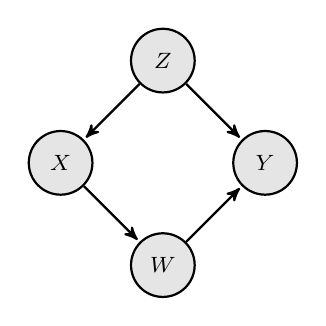
\begin{tikzpicture}[->,>=stealth',shorten >=1pt,auto,node distance=1cm,
  thick,main node/.style={observed}]
 %nodes
\node[main node](1){$Z$};
\node[main node, below left=of 1](2){$X$};
\node[main node, below right=of 1](3){$Y$};
\node[main node, below right=of 2](4){$W$};
 \path[every node/.style={font=\sffamily\small}]
    (1) edge (2) edge (3)
    (2) edge (4)
    (4) edge (3);
\end{tikzpicture} 
\end{subfigure}
\begin{subfigure}[t]{0.29\textwidth}
\centering
\caption{augmented graph $G^{\hat{X}}$}
\label{fig:rule3_augmented}
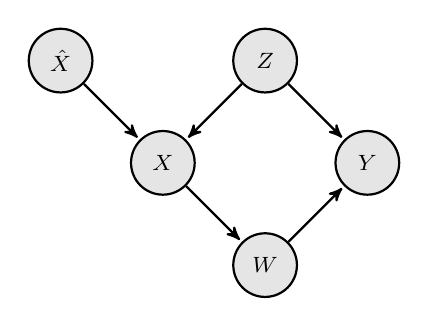
\begin{tikzpicture}[->,>=stealth',shorten >=1pt,auto,node distance=1cm,
  thick,main node/.style={observed}]
 %nodes
\node[main node](1){$Z$};
\node[main node, below left=of 1](2){$X$};
\node[main node, below right=of 1](3){$Y$};
\node[main node, below right=of 2](4){$W$};
\node[main node, above left=of 2](5){$\hat{X}$};
 \path[every node/.style={font=\sffamily\small}]
    (1) edge (2) edge (3)
    (2) edge (4)
    (4) edge (3)
    (5) edge (2);
\end{tikzpicture} 
\end{subfigure}
\begin{subfigure}[t]{0.29\textwidth}
\centering
\caption{$G_{\overline{X}}$}
\label{fig:rule3_after}
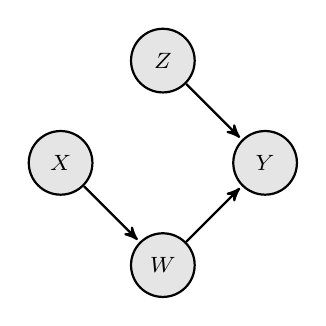
\begin{tikzpicture}[->,>=stealth',shorten >=1pt,auto,node distance=1cm,
  thick,main node/.style={observed}]
 %nodes
\node[main node](1){$Z$};
\node[main node, below left=of 1](2){$X$};
\node[main node, below right=of 1](3){$Y$};
\node[main node, below right=of 2](4){$W$};
 \path[every node/.style={font=\sffamily\small}]
    (1) edge (3)
    (2) edge (4)
    (4) edge (3);
\end{tikzpicture} 
\end{subfigure}
\caption{Example application of equation \ref{eq:Do3}. $(Y \ci \hat{X}|W,Z) \implies \P{Y|do(X),W,Z} = \P{Y|W,Z}$. We have to condition on $Z$ because conditioning on $W$ blocks the path $\hat{X}-X-W-Y$ but opens $\hat{X}-X-Z-Y$.}
\label{fig:rule3}
\end{figure}


\subsubsection{Identifiability}
A natural question to ask is, given a set of assumptions about the causal graph, is it possible to estimate a given interventional distribution from observational data? This is the identifiability problem. It asks if we can obtain an unbiased point estimate for the causal query of interest in the infinite data limit. A query is non-parametrically identifiable if it is identifiable without  assumptions about the functional form of the dependencies between variables in the graph.

\vspace*{.3cm}
\begin{definition}[Non-parametric identifiablity]
Let $G$ be a causal graph containing observed variables $\boldsymbol{V}$ and latent variables $\boldsymbol{U}$ and let $\P{\cdot}$ be any positive distribution over $\boldsymbol{V}$. A causal query of the form $\P{\boldsymbol{Y}|do(\boldsymbol{X}),\boldsymbol{W}}$, where $\boldsymbol{Y}$,$\boldsymbol{X}$ and $\boldsymbol{W}$ are disjoint subsets of $\boldsymbol{V}$, is non-parametrically identifiable if it is uniquely determined by $\P{\cdot}$ and $G$.
\end{definition} 

The question of non-parametric identifiability is solved. The do calculus is complete \citep{Shpitser2006b,Huang2006}. A problem is identifiable if and only if the interventional distribution of interest can be transformed into terms containing only observational quantities via repeated application of the do-calculus. There is a polynomial time algorithm \citep{Shpitser2006a} based on these properties that, for a given network and interventional (do-type) query, can:

\begin{enumerate}
\item determine if the query can be translated into an expression involving only distributions over observed variables. In other words, it can determine if the query is identifiable given the assumptions encoded by the network, and
\item if it is identifiable, return the required expression. 
\end{enumerate}

Figure \ref{fig:identify} shows some examples of identifiable and non-identifiable queries. I have created a javascript implementation of the identifiability algorithm \citep{Shpitser2006a} on which you can test your own queries http://finnhacks42.github.io.

\begin{figure}[h]
\centering
\begin{subfigure}[t]{0.29\textwidth}
\centering
\caption{}
\label{fig:id1}
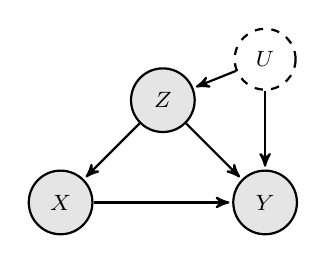
\begin{tikzpicture}[->,>=stealth',shorten >=1pt,auto,node distance=1cm,
  thick,lt/.style={latent},ob/.style={observed}]
\node[ob](1){$Z$};
\node[ob, below left=of 1](2){$X$};
\node[ob, below right=of 1](3){$Y$};
\node[lt,above=of 3](4){$U$};
 \path[every node/.style={font=\sffamily\small}]
    (1) edge (2) edge (3)
    (2) edge (3)
    (4) edge (1) edge (3);
\end{tikzpicture} 
\end{subfigure}
\begin{subfigure}[t]{0.29\textwidth}
\centering
\caption{}
\label{fig:id2}
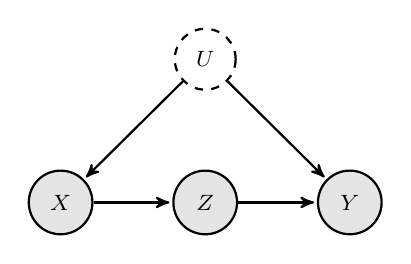
\begin{tikzpicture}[->,>=stealth',shorten >=1pt,auto,node distance=1cm,
  thick,lt/.style={latent},ob/.style={observed}]
\node[ob](1){$X$};
\node[ob, right=of 1](2){$Z$};
\node[ob, right=of 2](3){$Y$};
\node[lt,above=of 2](4){$U$};
 \path[every node/.style={font=\sffamily\small}]
    (1) edge (2)
    (2) edge (3)
    (4) edge (1) edge (3);
\end{tikzpicture} 
\end{subfigure}
\begin{subfigure}[t]{0.29\textwidth}
\centering
\caption{}
\label{fig:id3}
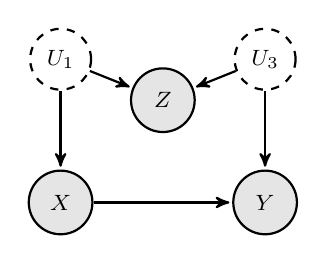
\begin{tikzpicture}[->,>=stealth',shorten >=1pt,auto,node distance=1cm,
  thick,lt/.style={latent},ob/.style={observed}]
\node[ob](1){$Z$};
\node[ob, below left=of 1](2){$X$};
\node[ob, below right=of 1](3){$Y$};
\node[lt,above=of 3](4){$U_3$};
\node[lt,above=of 2](5){$U_1$};
 \path[every node/.style={font=\sffamily\small}]
    (2) edge (3)
    (4) edge (1) edge (3)
    (5) edge (2) edge (1);
\end{tikzpicture} 
\end{subfigure}
\begin{subfigure}[t]{0.29\textwidth}
\centering
\vspace*{.5cm}
\caption{}
\label{fig:nid1}
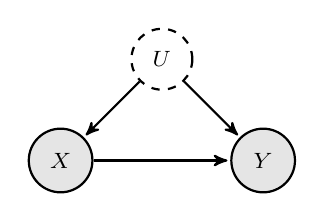
\begin{tikzpicture}[->,>=stealth',shorten >=1pt,auto,node distance=1cm,
  thick,lt/.style={latent},ob/.style={observed}]
\node[lt](1){$U$};
\node[ob, below left=of 1](2){$X$};
\node[ob, below right=of 1](3){$Y$};
 \path[every node/.style={font=\sffamily\small}]
    (1) edge (2) edge (3)
    (2) edge (3);
\end{tikzpicture} 
\end{subfigure}
\begin{subfigure}[t]{0.29\textwidth}
\centering
\vspace*{.5cm}
\caption{}
\label{fig:nid2_instrumental_variable}
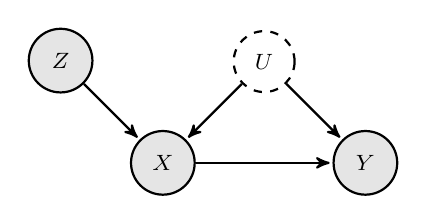
\begin{tikzpicture}[->,>=stealth',shorten >=1pt,auto,node distance=1cm,
  thick,lt/.style={latent},ob/.style={observed}]
\node[lt](1){$U$};
\node[ob, below left=of 1](2){$X$};
\node[ob, below right=of 1](3){$Y$};
\node[ob, above left=of 2](4){$Z$};
 \path[every node/.style={font=\sffamily\small}]
    (1) edge (2) edge (3)
    (2) edge (3)
    (4) edge (2);
\end{tikzpicture} 
\end{subfigure}
\begin{subfigure}[t]{0.29\textwidth}
\centering
\vspace*{.5cm}
\caption{}
\label{fig:nid3}
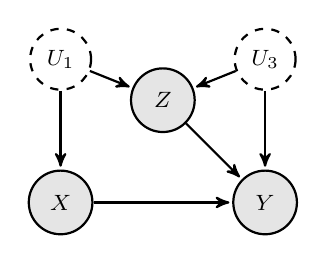
\begin{tikzpicture}[->,>=stealth',shorten >=1pt,auto,node distance=1cm,
  thick,lt/.style={latent},ob/.style={observed}]
\node[ob](1){$Z$};
\node[ob, below left=of 1](2){$X$};
\node[ob, below right=of 1](3){$Y$};
\node[lt,above=of 3](4){$U_3$};
\node[lt,above=of 2](5){$U_1$};
 \path[every node/.style={font=\sffamily\small}]
    (2) edge (3)
    (4) edge (1) edge (3)
    (5) edge (2) edge (1)
    (1) edge (3);
\end{tikzpicture} 
\end{subfigure}
\caption{Examples of identifiable and non-identifiable queries. In subfigures (a), (b) and (c) the causal query $\P{Y|do(X)}$ is identifiable. In subfigures (d), (e) and (f) it is not.}
\label{fig:identify}
\end{figure}


Many interesting questions relating to identifiability remain open. What is the minimal (by some metric) additional information that would be required to make a non-identifiable query identifiable? What if we assume various restrictions on the functional form of the relationships between the variables? Some queries that are not identifiable non-parametrically can be identified by additional assumptions, such as linearity. A complete algorithm for the problem of linear identifiability is yet to be found, despite a rich body of work \citep{Chen2016,tian2009parameter,drton2011global}.

Although identifiability is a natural and important question to ask, it does not partition causal questions into solvable and unsolvable. Estimators for identifiable queries can be slow to converge and we may be able to obtain useful bounds on causal effects in cases where point estimates are not identified.

\subsection{Defining causal effects} 
\label{sec:defining-causal-effects}
So far we have described causal effect estimation in term of identifying the interventional distribution $\P{Y|do(X)}$ from observational data. This interventional distribution is in fact a family of distributions parameterised by the value, $x$, to which the treatment variable $X$ is set. From a decision theoretic viewpoint, we can select an optimal action $x$ by specifying a utility function $\mathcal{U}:y \in \mathcal{Y} \rightarrow \mathbb{R}$ that assigns a value to each outcome $y$ and then selecting the action that maximises the expected utility. 

\eqn{
\label{eqn:utility_max}
x* =\argmax_x \Esub{y\sim\P{Y|do(X=x)}}{{\cal{U}}(y)}
} 

Frequently however, studies wish to define and estimate a causal effect without reference to a specific utility function. There are several ways of defining causal effects that can be viewed as different ways of summarising the family of interventional distributions. For a binary treatment variable $X$, the average causal effect, ACE \footnote{Also referred to as the average treatment effect (ATE)} is defined as:

\eqn{
\label{eqn:ACE}
ACE = \E{Y|do(X = 1)} - \E{Y|do(X=0)}
}

Assuming the expectations in equation \ref{eqn:ACE} are well defined, the ACE captures the shift in the mean outcome that arises from varying $X$. It does not capture changes in variance or higher moments of the distribution. The ACE can be generalised to non-discrete interventions by considering the effect on the expectation of $Y$ of an infinitesimal change in $x$. If $X$ is linearly related to $Y$ then the ACE is constant and equivalent to the corresponding coefficient in the linear structural equation model. 

\eqn{
\label{eqn:ACE_continuous}
ACE(x) = \frac{d}{dx}\E{Y|do(X=x)}
}


The average causal effect is often introduced as the average over individual causal effects as discussed in section \ref{sec:counterfactuals}. Individual causal effects are deterministic and cannot be expressed as properties of the interventional distribution. However, we can personalise the average causal effect by stating it with respect to some observed context. I will refer to this as the personalised causal effect (PCE).\footnote{This quantity is sometimes called the conditional average treatment effect (CATE). However, that term is also used for the sample rather than population effect.} 

\eqn{
PCE(z) = \E{Y|do(X=1),z} - \E{Y|do(X=0),z}
}

In some cases, the average causal effect for some sub-group of the population is of prime interest. A particularly common example of this is the average treatment effect of the treatment of the treated (ATT). This would be the key quantity of interest if we had to decide whether or not to continue providing a program or treatment for which we could not control the treatment assignment process. 

\eqn{
ATT = \Esub{z\sim \P{Z|x=1}}{Y|do(X = 1)} - \Esub{z\sim \P{Z|x=1}}{Y|do(X=0)}
}

Causal effects can also be written in terms of counterfactuals. The ACE is $\E{\cf{Y}{1} - \cf{Y}{0}}$. We could estimate the ratio of expectations $\frac{\E{\cf{Y}{1}}}{\E{\cf{Y}{0}}}$ instead of the difference. However, the quantity   $\E{\frac{\cf{Y}{1}}{\cf{Y}{0}}}$ depends on the joint distribution over the counterfactual variables $(\cf{Y}{1},\cf{Y}{0})$ and thus cannot be computed from the interventional distribution. 

Another way of conceptualising causal effects is as a property indicating the strength of the causal link between two variables. This notion is complex to formalise when the relationship between variables is non-linear. Suppose $Y = X \oplus Z$ with $P(Z=1)=\frac{1}{2}$, the interventional distributions over $X$ are identical after marginalising out $Z$. \citet{Janzing2013} propose a number of postulates that a notion of causal strength could satisfy, demonstrate why previous measures fail these postulates and propose an alternative based on information flow. 


\subsection{Estimating causal effects by adjusting for confounding variables}
\label{sec:causal_effect_under_ignorability}
Probably the two most frequently applied approaches to estimating causal effects from observational data are instrumental variables and adjusting for confounding factors. Instrumental variables correspond to the graph in figure \ref{fig:nid2_instrumental_variable}, which is not identifiable without parametric assumptions, however they can provide tight bounds. Adjusting for confounding equates to identifying a set of variables $\boldsymbol{Z}$ such that the ignorability assumption discussed in section \ref{sec:counterfactuals} holds. This corresponds to a simple graphical test known as the backdoor criterion \citep{Pearl2000}. The setting is also referred to as unconfounded. 

\vspace*{0.3cm}
\begin{theorem}[The backdoor criterion]\citep{Pearl2000}
Let $\boldsymbol{X}$, $\boldsymbol{Z}$ and $\boldsymbol{Y}$ be disjoint sets of vertices in a causal graph $G$. If $\boldsymbol{Z}$ blocks (see Definition \ref{def:unblocked}) for every path from $X_i$ to $Y_j$ that contains a link into $X_i$, for every pair $(X_i \in \boldsymbol{X},Y_j \in \boldsymbol{Y})$, and no node in $\boldsymbol{Z}$ is a decedent of a node in $\boldsymbol{X}$ then the backdoor criterion is satisfied and;

\eqn{
\label{eqn:backdoor}
\P{\boldsymbol{y}|do(\boldsymbol{x})} =\sum_{\boldsymbol{z}} \P{\boldsymbol{y}|\boldsymbol{x},\boldsymbol{z}}\P{\boldsymbol{z}}
}
\end{theorem}

The backdoor criterion derives from rule 2 of the do-calculus. Selecting which covariates should be adjusted for to estimate a causal effect reduces to identifying a set that satisfies the backdoor criterion. There may be more than one valid adjustment set, (figure \ref{fig:adjust_multiple}). The seemingly simple problem of determining if a variable should be adjusted for when estimating causal effects has been the subject of substantial debate and controversy \citep{pearl2009myth}. Adjusting for the wrong variables (even pre-treatment variables) can introduce or magnify bias, see figure \ref{fig:m-graph}. Causal graphs and the back door criterion provide a clear mechanism for deciding which variables should be adjusted for. For a practical example, see the discussion in \citet{schisterman2009overadjustment} on whether estimates of the causal effect of smoking on neonatal mortality should adjust for birth weight.

\begin{figure}
\centering
\begin{subfigure}[t]{0.48\textwidth}
\centering
\caption{Multiple valid adjustment sets.}
\label{fig:adjust_multiple}
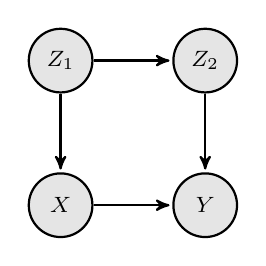
\begin{tikzpicture}[->,>=stealth',shorten >=1pt,auto,node distance=1cm,
  thick,lt/.style={latent},ob/.style={observed}]
\node[ob](2){$X$};
\node[ob, right=of 2](3){$Y$};
\node[ob,above=of 3](4){$Z_2$};
\node[ob,above=of 2](5){$Z_1$};
 \path[every node/.style={font=\sffamily\small}]
    (2) edge (3)
    (5) edge (2) edge (4)
    (4) edge (3);
\end{tikzpicture} 
\end{subfigure}
\begin{subfigure}[t]{0.48\textwidth}
\centering
\caption{Don't condition on all observable variables}
\label{fig:m-graph}
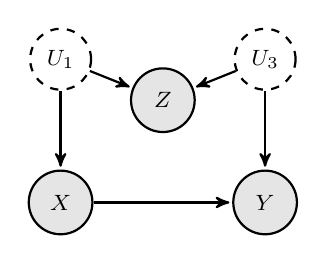
\begin{tikzpicture}[->,>=stealth',shorten >=1pt,auto,node distance=1cm,
  thick,lt/.style={latent},ob/.style={observed}]
\node[ob](1){$Z$};
\node[ob, below left=of 1](2){$X$};
\node[ob, below right=of 1](3){$Y$};
\node[lt,above=of 3](4){$U_3$};
\node[lt,above=of 2](5){$U_1$};
 \path[every node/.style={font=\sffamily\small}]
    (2) edge (3)
    (4) edge (1) edge (3)
    (5) edge (2) edge (1);
\end{tikzpicture} 
\end{subfigure}
\caption{Identifying an optimal adjustment set is not always intuitively obvious. There may be multiple valid adjustment sets. In sub-figure (a) $Z_1$ or $Z_2$ or $\set{Z_1,Z_2}$ all block the backdoor path from $X$ to $Y$. Adding additional variables (even pre-treatment variables) to a valid adjustment set can result in an invalid set as in sub-figure (b). In this case the empty set is a valid adjustment set for the causal effect of $X$ on $Y$. However adding $Z$ would open a backdoor path $X-U_1-Z-U_2-Y$}
\label{fig:adjustment}
\end{figure}

Given that a set of variables $\boldsymbol{Z}$ satisfies the backdoor criterion (or equivalently the conditional ignorability assumption), the interventional distribution is asymptotically identifiable and can be estimated from equation \ref{eqn:backdoor}. The expected value of $Y$ after the intervention $do(X=x)$ is given by equation \ref{eqn:expected_post_intervention} and the average causal effect for a binary intervention $x \in \set{0,1}$ is given by equation \ref{eqn:ace_ignoreable}.

\eqn{
\label{eqn:expected_post_intervention}
\E{Y|do(X=x)} = \Esub{z\sim \P{\vb{Z}}}{\E{Y|x,\vb{z}}}
} 

\eqn{
\label{eqn:ace_ignoreable}
ACE = \Esub{z\sim \P{\vb{Z}}}{\E{Y|1,\vb{z}}-\E{Y|0,\vb{z}}}
}  

Assuming $x$ and $\vb{z}$ are discrete, equation \ref{eqn:expected_post_intervention}, and thus the ACE, can be estimated by selecting the data for which $X=x$, stratifying by $\vb{Z}$, then computing the mean outcome within each stratum and finally weighting the results by the number of samples in each strata. However this approach is not workable for most real world problems with finite samples as the number of strata grows exponentially with the dimension of $\vb{Z}$ and it cannot handle continuous covariates. There is a substantial body of work within in the statistics and econometrics literature on estimating average causal effects assuming conditional ignorability (see \citet{Imbens2004} for a comprehensive review). The key approaches are based on matching on covariates, propensity score methods and regression. We now examine these approaches from a machine learning perceptive. 

In standard supervised learning, we have a training set $(\vb{x_1},y_1),...,(\vb{x_n},y_n)$ assumed to be sampled i.i.d from an unknown distribution $\P{\vb{x},y} =\P{\vb{x}}\P{y|\vb{x}}$. The goal is to select a hypothesis $h \in \mathcal{H} : \mathcal{X} \rightarrow \mathcal{Y}$ such that, on unseen data $ \sim \P{\vb{x},y}$, $h(\vb{x})$ is close (by some metric) in expectation to $y$. In other words we wish to minimise the generalisation error $E_{out}(h)$,

\eqn{
E_{out}(h) = \Esub{(\vb{x},y)\sim \P{\vb{x}}\P{y|\vb{x}}}{L(h(\vb{x}),y)}
}

We cannot directly compute the generalisation error as $\P{\vb{x},y}$ is unknown, as we only have access to a sample. We could search over $\mathcal{H}$ and select a hypothesis $h^*(\vb{x})$ that minimises some loss function on the sample data.

\eqn{
E_{in}(h) = \frac{1}{n}\sum_{i=1}^n L(h(\vb{x}_i),y_i)
}

The VC-dimension of the hypothesis space provides (typically loose) bounds on the probability that $E_{out} >> E_{in}$. However, in practice, the generalisation error is usually estimated empirically from a hold-out set of the sample that was not used to train the model, or via cross-validation. 

In the causal effect estimation under ignorability, we have training data $(\vb{x}_1,\vb{z}_1,y_1),...,(\vb{x}_n,\vb{z}_n,y_n)$ sampled i.i.d from $\P{\vb{z}}\P{\vb{x}|\vb{z}}\P{y|\vb{x},\vb{z}}$. Estimating $\E{Y|do(\vb{X}=\vb{x})}$ corresponds to selecting a hypothesis $h \in \mathcal{H}:\mathcal{X} \times \mathcal{Z} \rightarrow \mathcal{Y}$ that minimises;

\eqn{
\label{eqn:causal_covariate_shift}
E_{out} &= \Esub{(\vb{x},\vb{z},y)\sim \delta(\vb{x}-\vb{x'})\P{\vb{z}}\P{y|\vb{x},\vb{z}}}{L_2(h(\vb{x},\vb{z}),y)},\\
&= \Esub{(\vb{z},y)\sim \P{\vb{z}}\P{y|\vb{x},\vb{z}}}{L_2(h(\vb{x},\vb{z}),y)},
}

\citet{Johansson2016_counterfactual_rep} identified that this is equivalent to the covariate shift problem. If we let $\vb{v} = (\vb{x},\vb{z})$ then we have training data sampled from $\Pns{train}{\vb{v}}\P{y|\vb{v}}$ where $\Pns{train}{\vb{v}}=\P{\vb{z}}\P{\vb{x}|\vb{z}}$, but at test time the data will be sampled from $\Pns{test}{\vb{v}}\P{y|\vb{v}}$, where $\Pns{test}{\vb{v}} = \delta(\vb{x}-\vb{x'})\P{\vb{z}}$. \footnote{It is not obvious that the question of estimating causal effects under ignorability entirely reduces to  covariate shift. Take the case where we have a binary intervention $x \in \set{0,1}$. Suppose we learn $h(1,\vb{z}) = \E{Y|x=1,\vb{z}}+g(\vb{z})$ and $h(0,\vb{z}) = \E{Y|x=0,\vb{z}}+g(\vb{z})$, then the estimated average causal effect equals the true average causal effect for any function $g$, $\E{h(1,\vb{z})-h(0,\vb{z})} = \E{Y|x=1,\vb{z}} - \E{Y|x=0,\vb{z}}$. More generally, if the goal is to select an optimal action $x^*$ from a continuous space of possible interventions we need algorithms capable of leveraging any structure in the relationship between $x$ and $y$ as well as a means of focusing the loss on regions of the sample likely to affect $x^*$.} With this connection to covariate shift in mind, let us return to regression, matching and propensity scores. 

\subsubsection{Regression}

The regression approach is to learn a function that is a good approximation to the output surface $\E{Y|X,Z}$. Let $f_1(z)= \E{Y|X=1,Z=z}$. The expectation of $Y$ after the intervention $X=1$ is then obtained by taking the expectation with respect to $Z$, $\E{Y|do(X=1)} = \Esub{z \sim \P{Z}}{\E{Y|X=1,z}}$. We can learn a parametric regression model $\hat{f}_1(z)$ via empirical risk minimisation. 

\eqn{
\hat{f}_1(z) = h_1(z;\hat{\theta}_{obs}) \text{, where } \hat{\theta}_{obs} = \argmin_{\theta \in \Theta}\left[\frac{1}{n}\sum_{i=1}^n \ind{x_i=1} L\left(h_1(z_i;\theta),y_i\right)  \right]
}

This estimator is consistent with respect to the observational distribution. As the sample size tends to infinity, $\hat{\theta}_{obs}$ approaches the parameter within the hypothesis space that minimises the expected loss given data sampled from the observational distribution. 

\eqn{
\lim_{n \rightarrow \infty}\hat{\theta}_{obs} = \argmin_{\theta \in \Theta} \Esub{(z,y) \sim \P{z|x=1}\P{y|x=1,z}}{L\left(h_1(z;\theta),y \right)}
}

If the model is correctly specified such that $f_1(z) = h_1(z;\theta^*)$ for some  $\theta^* \in \Theta$ then the empirical risk minimisation estimate is consistent with respect to the loss over any distribution of $Z$  \citep{Sugiyama2007}, including the interventional one. 

\eqn{
\lim_{n \rightarrow \infty}\hat{\theta}_{obs} = \theta^* = \argmin_{\theta \in \Theta} \Esub{(z,y) \sim \P{z}\P{y|x=1,z}}{L\left(h_1(z;\theta),y \right)}
}

The average causal effect can then be estimated by:

\eqn{
\label{eqn:cef_empirical_regression}
\hat{\tau}_{reg} = \sum_{i=1}^n \left(\hat{f}_1(z_i) - \hat{f}_0(z_i)\right)
}

Regression thus has a direct causal interpretation if the parametric model is correctly specified and the covariates included form a valid backdoor adjustment set for the treatment variable of interest in the corresponding structural equation model. 

\subsubsection{Propensity scores}
If the parametric model is miss-specified then the parameter that minimises the loss depends on the distribution from which the covariates $z$ are sampled. The model learned by ERM could perform very well in a validation set (which estimates the generalisation error over the observational distribution of $(x,z)$) but yield very poor estimates of the causal effect, see figure \ref{fig:covariate_shift_adjust}. 


\begin{figure}[h]
\centering
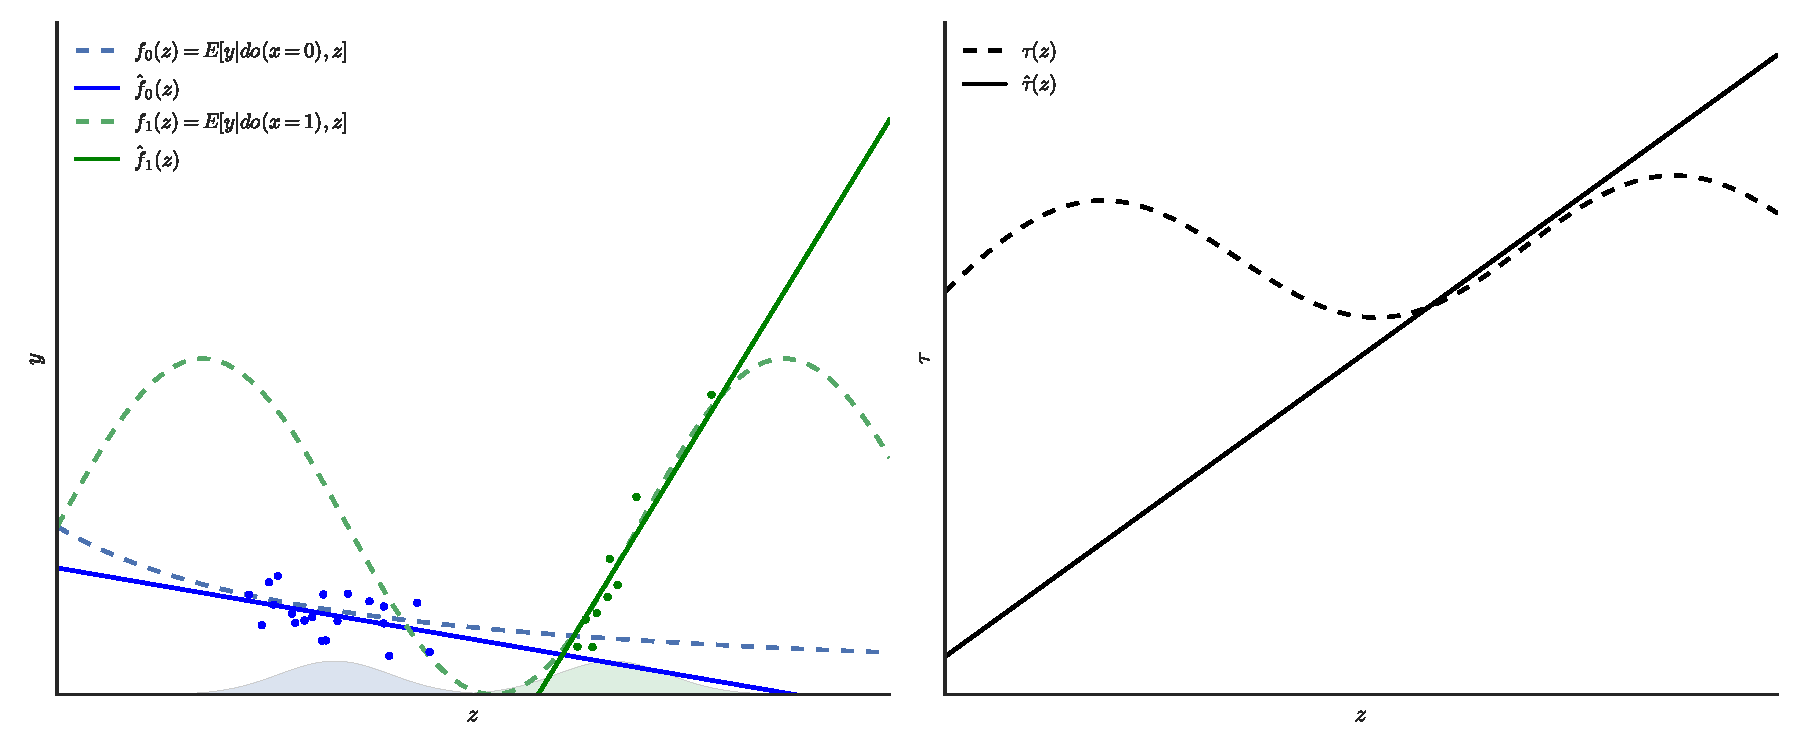
\includegraphics[scale=.55]{covariate_shift_estimation.pdf}
\caption{
Parametric regression may yield poor estimates of causal effects if the model is miss-specified, even if the model fits well over the domain of the training data. In this example, $\P{Z|X=0} \sim N(\mu_0,\sigma_0^2)$ and $\P{Z|X=1} \sim N(\mu_1,\sigma_1^2)$ with little overlap in the densities. If $X=0$ then $Y \sim N(f_1(x)=sin(x),\sigma_y^2)$ and if $X=1$ then $Y \sim N(f_0(x) = \frac{1}{x+1},\sigma_y^2)$. We estimate $f_1(z)$ from the sample in which $X=1$ (green points) and $f_0(z)$ from the sample for which $X=0$ (blue points). In both cases the linear model is a good fit to the data. However, the resulting estimate of the causal effect is very poor for the lower values of $z$. } 
\label{fig:covariate_shift_adjust}
\end{figure}


A general approach to estimating the expectation of some function $f(\cdot)$ with respect to data from some distribution $\P{\cdot}$, when we have data sampled from a different distribution $\Q{\cdot}$ is importance sampling \citep{horvitz1952generalization,Koller2009}. 
\eqn{
\label{eqn:importance_sampling}
\Esub{\vb{v} \sim \P{\vb{v}}}{f(v)} = \Esub{\vb{v} \sim \Q{\vb{v}}}{f(v)\frac{\P{\vb{v}}}{\Q{\vb{v}}}}
}

This importance weighting approach can be applied to the covariate shift/average causal effect problem by weighting the terms in the empirical risk minimisation estimator \citep{Sugiyama2007}.

\eqn{
\label{eqn:importance_weighted_erm}
\hat{\theta}_{iw} &= \argmin_{\theta \in \Theta}\left[\frac{1}{n}\sum_{i=1}^n \ind{x_i=1} L\left(h_1(z_i;\theta),y_i\right)\frac{\P{z_i}\delta(x_i-1)}{\P{z_i}\P{x_i=1|z_i}}  \right] \\
&= \argmin_{\theta \in \Theta}\left[\frac{1}{n}\sum_{i=1}^n \ind{x_i=1} L\left(h_1(z_i;\theta),y_i\right)\frac{1}{e(z_i)}  \right],
}

where $e(\vb{z})$ is the propensity score, defined by \citep{Rosenbaum1983};
\eqn{
e(\vb{z})\equiv \P{x=1|\vb{z}}
}

The estimator in equation \ref{eqn:importance_weighted_erm} is an example of a doubly robust estimator \citep{scharfstein1999adjusting,}. Doubly robust methods are asymptotically unbiased so long as either the regression model $h$ or propensity score $e$ are correctly specified \citep{robins1995semiparametric}. 

The propensity score can be used to estimate the average causal effect without specifying a regression model for $\E{Y|X,\vb{Z}}$. \citet{Rosenbaum1983} demonstrated that if the ignorability assumption is satisfied by conditioning on $\vb{Z}$, then it is also satisfied by conditioning on $e(\vb{z})$. This allows for estimators based on stratifying, matching or regression on the propensity score rather than the covariates $\vb{Z}$. Inverse propensity weighting can also be combined with empirical estimation of $\E{Y|X,Z}$ yielding the simple, albeit inefficient, estimator in equation \ref{eqn:simple_inverse_propensity} \citep{Imbens2004}. In some settings, such as stratified randomised trials \citep{imbens2015causal} or learning from logged bandit feedback \citep{Bottou2013}, the propensity score may be known. However, in general, it must be estimated from data. Frequently this is undertaken with a simple parametric model, such as logistic regression, but a wide range of standard machine learning algorithms including bagging and boosting, random forests and neural networks can also be applied   \citep{Austin2011}. \citet{Lunceford2004} review the theoretical properties of key propensity score based estimators, including stratification and inverse propensity weighting. 

\eqn{
\E{Y|do(X=x)} = \Esub{z\sim \P{\vb{Z}}}{\E{Y|x,\vb{z}}} = \Esub{z\sim \P{\vb{Z|x}}}{\E{Y|x,\vb{z}}\frac{1}{e(\vb{z})}}
}

\eqn{
\label{eqn:simple_inverse_propensity}
\hat{\tau}_{ip} = \frac{1}{n}\sum_{i=1}^n \left(\frac{\ind{x_i=1}y_i}{e(\vb{z}_i)} -\frac{\ind{x_i=0}y_i}{1-e(\vb{z}_i)}\right)
}


\subsubsection{Matching}
There is a straightforward connection between matching and regression for causal effect estimation. If $h \in \mathcal{H} \implies h + a \in \mathcal{H}$ for any constant $a$ and $\hat{f}$ is selected by minimising empirical risk with an $L_2$ loss then $\frac{1}{n}\sum_{i=1}^n \ind{x_i=1}\hat{f}_1(z_i) = \frac{1}{n}\sum_{i=1}^n \ind{x_i=1}y_i$ \footnote{\citep{Imbens2004} state this holds for most implementations}, and equation \ref{eqn:cef_empirical_regression} can be re-written as: 

\eqn{
\label{eqn:cef_regression_missing}
\hat{\tau}_{reg} = \sum_{i=1}^n \left[\ind{x_i=1}\left(y_i - \hat{f}_0(z_i)\right) +\ind{x_i=0}\left(\hat{f}_1(z_i) - y_i \right)\right]
}

This formulation of the regression estimator highlights the missing data aspect of casual effect estimation. For each instance, the regression models are used to estimate the counterfactual outcome had the instance received the alternate treatment. Matching estimates the counterfactual outcome for an instance from the outcome of \emph{similar} instances that received a different treatment. \citet{abadie2002simple} analyse an estimator where both target and control instances are matched and the matching is done with replacement, let $j \in J_k(i)$ be the indices of the $k$ instances closest to $i$ by some metric $d(z_i,z_j)$ such that $x_i \neq x_j$.

\eqn{
\hat{\tau}_{match} = \sum_{i=1}^n \left[\ind{x_i=1}\left(y_i - \frac{1}{k}\sum_{j \in J_k(i)}y_j\right) +\ind{x_i=0}\left(\frac{1}{k}\sum_{j \in J_k(i)}y_j - y_i \right)\right]
}

This estimator is equivalent to equation \ref{eqn:cef_regression_missing} with k nearest neighbour regression. There are many variants of matching estimators using different distance metrics, matching with or without replacement (and in the latter case, greedy or optimal matching) and with or without discarding matches beyond some threshold \citep{Cochran1973,rosenbaum1985constructing}. Although intuitive, matching estimators in general have poor large sample properties \citep{Abadie2006}. An exception is where the goal is to estimate the average treatment effect of treatment on the treated in settings where there is a large set of control instances (compared to treatment instances) \citep{Imbens2004}. 

The practical performance of the estimation approaches discussed in this section depend on the sample size, dimensionality of the covariates, the complexity of the treatment assignment mechanism and output function, and the degree of prior knowledge available about these functions. A key difference between standard machine learning problems and causal effect estimation is that when estimating causal effects we cannot directly apply cross-validation or a hold-out set for model selection because we lack samples from the counterfactual. 

The significance of this should not be underestimated. Cross-validation has allowed applied machine learning to succeed with a very atheoretical approach on the basis that we can identify when a model is successful. With causal effect estimation there is no guarantee that a model that performs well at prediction (even out of sample) will accurately estimate the outcome of an intervention. \citet{Sugiyama2007} propose inverse propensity weighted cross validation for the covariate shift problem. There is relatively little theory on model selection for estimating the propensity score. To achieve asymptotically unbiased estimates, the covariates should satisfy the backdoor criterion. It is also known that conditioning on instrumental variables, which directly influence $X$ but not $Y$, increases variance without any reduction in bias and can increase bias if there are unmeasured confounding variables \citep{Wooldridge2009,Bhattacharya2012,Pearl2012b,Myers2011}. With doubly robust estimators, one could apply an iterative approach, fitting a propensity score model, using the results for inverse propensity weighted cross-validation of the regression model and then selecting covariates for the propensity model on the assumption the estimated regression function was correct. I have found no examples of such an approach.

The performance of methods for causal effect estimation can be tested on simulated data \citep{Frolich2001,zhao2004using,Hill2011,Dorie2016} or by comparing estimates from observational studies with the results from corresponding experiments \citep{lalonde1986evaluating,Fraker1987,heckman1997matching,heckman1998characterizing,dehejia1999causal,Smith2001,Anglemyer2014}. Unfortunately, there are a relatively small number of examples where comparable observational and experimental data are available. The results are mixed with later studies finding generally better alignment of results, but it is hard to ascertain if this is due to improved methodological approaches or over-fitting to the available data.  

\section{Bayesian reasoning and causality}
\label{sec:bayesian_causality}
The Bayesian approach to modelling encapsulates a very general approach to combining prior knowledge and assumptions with data to draw inferences. You can specify a complex model that captures your assumptions about the underlying mechanisms of your system, describe uncertainty about the parameters (and priors over their values), and then update your beliefs about the values of these parameters based on the observed data. If you believe the model to be a mechanistic representation of the way the world works then it can be used to infer the consequences of interventions.

Why then do we need a special framework for causal inference? Why not encode all the assumptions required to infer the outcome of an intervention in a given system in a Bayesian model? The short answer is we could. However, causal graphical models represent a useful level of abstraction for many problems. Formalising the definition of an intervention within the framework of causal graphical models provides us with an explicit mechanism to map information from one data generating process, the system pre-intervention, to another, the system post-intervention. We do not need to specify the functional relationships between the variables or priors over their distributions. The power of defining an intervention in this way stems from the number of things that are assumed invariant between the two processes. All the (conditional) distributions for variables in the graph that were not directly set by the intervention are assumed not be changed by it. The causal framework also provides, via the do-calculus, a rigorous method to draw a boundary around which variables we must measure and model to identify causal effects.  

We can represent problems where the goal is to infer properties of the post-interventional system based on data generated by the pre-interventional distribution by explicitly representing both systems and their common features (figure \ref{fig:causal_ordinary_bayes}). This does not require any special framework or notation. The graphs in figure  \ref{fig:causal_ordinary_bayes} are ordinary Bayesian networks. However, without a causal framework, we have to make assumptions about what will be invariant to the intervention for each such problem encountered. For complex problems, it is very difficult to conceptualise the assumptions we expect to hold without the benefit of a causal framework.  

\begin{figure}[h]
\center
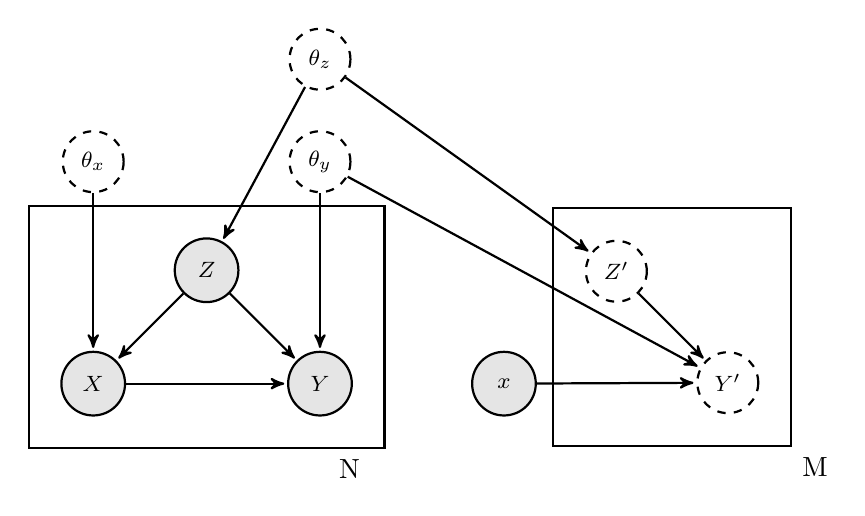
\begin{tikzpicture}[->,>=stealth',shorten >=1pt,auto,node distance=1.2cm, thick,node/.style={observed},lt/.style={latent}]
\tikzstyle{box}=[rectangle, draw=black!100]
 %nodes
\node[node](1){$Z$};
\node[node, below left=of 1](2){$X$};
\node[node, below right=of 1](3){$Y$};
\node[node, right=1.5cm of 3](4){$x$};
\node[lt, above right=of 4](5){$Z'$};
\node[lt, below right=of 5](6){$Y'$};
\node[lt, above=2.0cm of 3](9){$\theta_{y}$};
\node[lt, above=0.5cm of 9](7){$\theta_z$};
\node[lt, above=2.0cm of 2](8){$\theta_x$};
\path[every node/.style={font=\sffamily\small}]
    (1) edge (2) edge (3)
    (2) edge (3)
    (4) edge (6)
    (5) edge (6)
    (8) edge (2)
    (7) edge (1) edge (5)
    (9) edge (3) edge (6);
\node[rectangle, inner sep=4.0mm, fit= (1) (2) (3),draw=black!100,label=below right:N] {};
\node[rectangle, inner sep=4.0mm, fit= (5) (6),draw=black!100,label=below right:M] {};
\end{tikzpicture} 
\caption{Causal inference with ordinary Bayesian networks. The plate on the left represents the observed data generated prior to the intervention and the plate on the right the data we anticipate obtaining after an intervention that sets the pre-interventional variable $X$ to $x$. The assumptions characterised by this plate model correspond to those implied by the causal Bayesian network in figure \ref{fig:causal_adjust} for the intervention $do(X=x)$. As the networks in this figure are ordinary Bayesian networks, we could have represented the same information with a different ordering of the links within each plate. However, this would then entail a complex transformation relating the parameters between the two plates, rather than a simple invariance.}
\label{fig:causal_ordinary_bayes}
\end{figure}

Causal graphical models can also be combined with Bayesian approaches to estimation. For example, we can use a causal graphical model to identify a set of variables that form a valid adjustment set and then use Bayesian regression to estimate posterior distribution over a given causal effect. However, as I highlight in the next section, the way priors are specified is critical.

\subsection{Careful with that prior}

Suppose data is generated by the linear Gaussian Bayesian network below. The goal is to estimate the causal effect of $X$ on $Y$, that is identifying the value of the coefficient $w_{yx}$. The variable $U$ is latent. 

\eqn{
\P{U} &= N(0 , v_u) \\
\label{eqn:careful_with_priors}
\P{Z|U} &= N(w_{zu}U , v_z) \\
\P{X|Z} &= N(w_{xz}Z , v_x) \\
\P{Y|U,Z,X} & = N(w_{yu}U +w_{yz}Z + w_{yx}X , v_y)
}

\begin{figure}[h]
\centering
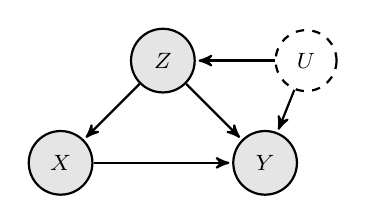
\begin{tikzpicture}[->,>=stealth',shorten >=1pt,auto,node distance=1cm,
  thick,main node/.style={observed},lt/.style={latent}]

 %nodes
\node[main node](1){$Z$};
\node[main node, below left=of 1](2){$X$};
\node[main node, below right=of 1](3){$Y$};
\node[lt, right=of 1](4){$U$};


 \path[every node/.style={font=\sffamily\small}]
    (1) edge (2)
    	edge (3)
    (2) edge (3)
    (4) edge (1) edge (3);
	
\end{tikzpicture} 
\caption{ }
\label{fig:careful_with_priors}
\end{figure}

As each variable is a linear function of its parents, with Gaussian noise, resulting in a joint distribution $\P{U,Z,X,Y}$ that is multivariate normal. Marginalising out $U$ and conditioning on $X$ and $Z$ yields,

\eqn{
Y \sim N(w_{yx} X + \beta Z, \epsilon) 
}

where

\eqn{
\beta &= w_{yz}+\frac{w_{yu}w_{zu}}{w_{zu}^2+\frac{v_z}{v_u}}, \text{ and}\\
\epsilon &= v_y + w_{yu}^2v_u - \frac{v_u^2 w_{zu}^2 w_{yu}^2 }{v_z^2+v_u^2 w_{zu}^2}
}

The causal effect of $X$ on $Y$ is identifiable (even without the linear Gaussian assumptions) as $Z$ satisfies the backdoor criterion and the expectation of the coefficient for $X$ in a standard OLS regression of $Y$ against $X$ and $Z$ is $w_{yx}$. However, the causal effect of $Z$ on $Y$ is not identifiable due the presence of the unobserved confounder $U$. The coefficient $\beta$ captures both the causal relationship between $Z$ and $Y$, $w_{yz}$ and the indirect relationship through $U$, which we cannot separate without observing $U$. 

Undertaking a Bayesian regression of $X$ and $Z$ against $Y$ and using intuition based on the causal relationship between $Z$ and $Y$ to select a prior for $\beta$ will lead to selection of something centered around $w_{yz}$. However, this is incorrect and can introduce bias into our estimate of the coefficient for $w_{yx}$, as demonstrated in figure \ref{fig:careful-prior-example}. The prior for $\beta$ should be based on the belief about how $Z$ is expected to be \emph{associated} with $Y$, after marginalising out any confounding variables. 

\begin{figure}[h]
\begin{subfigure}[t]{0.99\textwidth}
     \caption{No prior on $\beta$, the posterior on $w_{yx}$ is centered around its true value}
    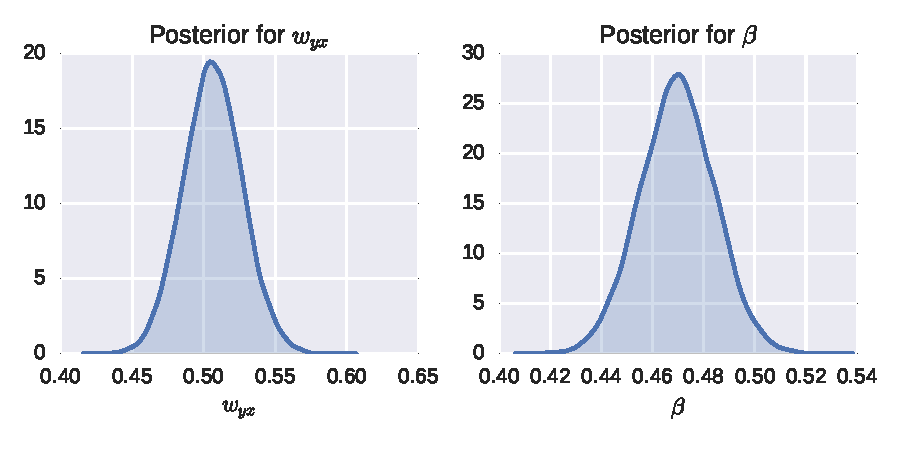
\includegraphics[scale=1]{prior_no_prior}
\end{subfigure}
\begin{subfigure}[t]{0.99\textwidth}
     \caption{Prior on $\beta$ centered around $w_{yz}$, the causal effect of $Z$ on $Y$, $Prior(\beta)= N(w_{yz},\sigma = 0.5)$. The posterior on $w_{yx}$ is biased away from its true value (as is the posterior on $\beta$ but this is not the key quantity of interest).}
    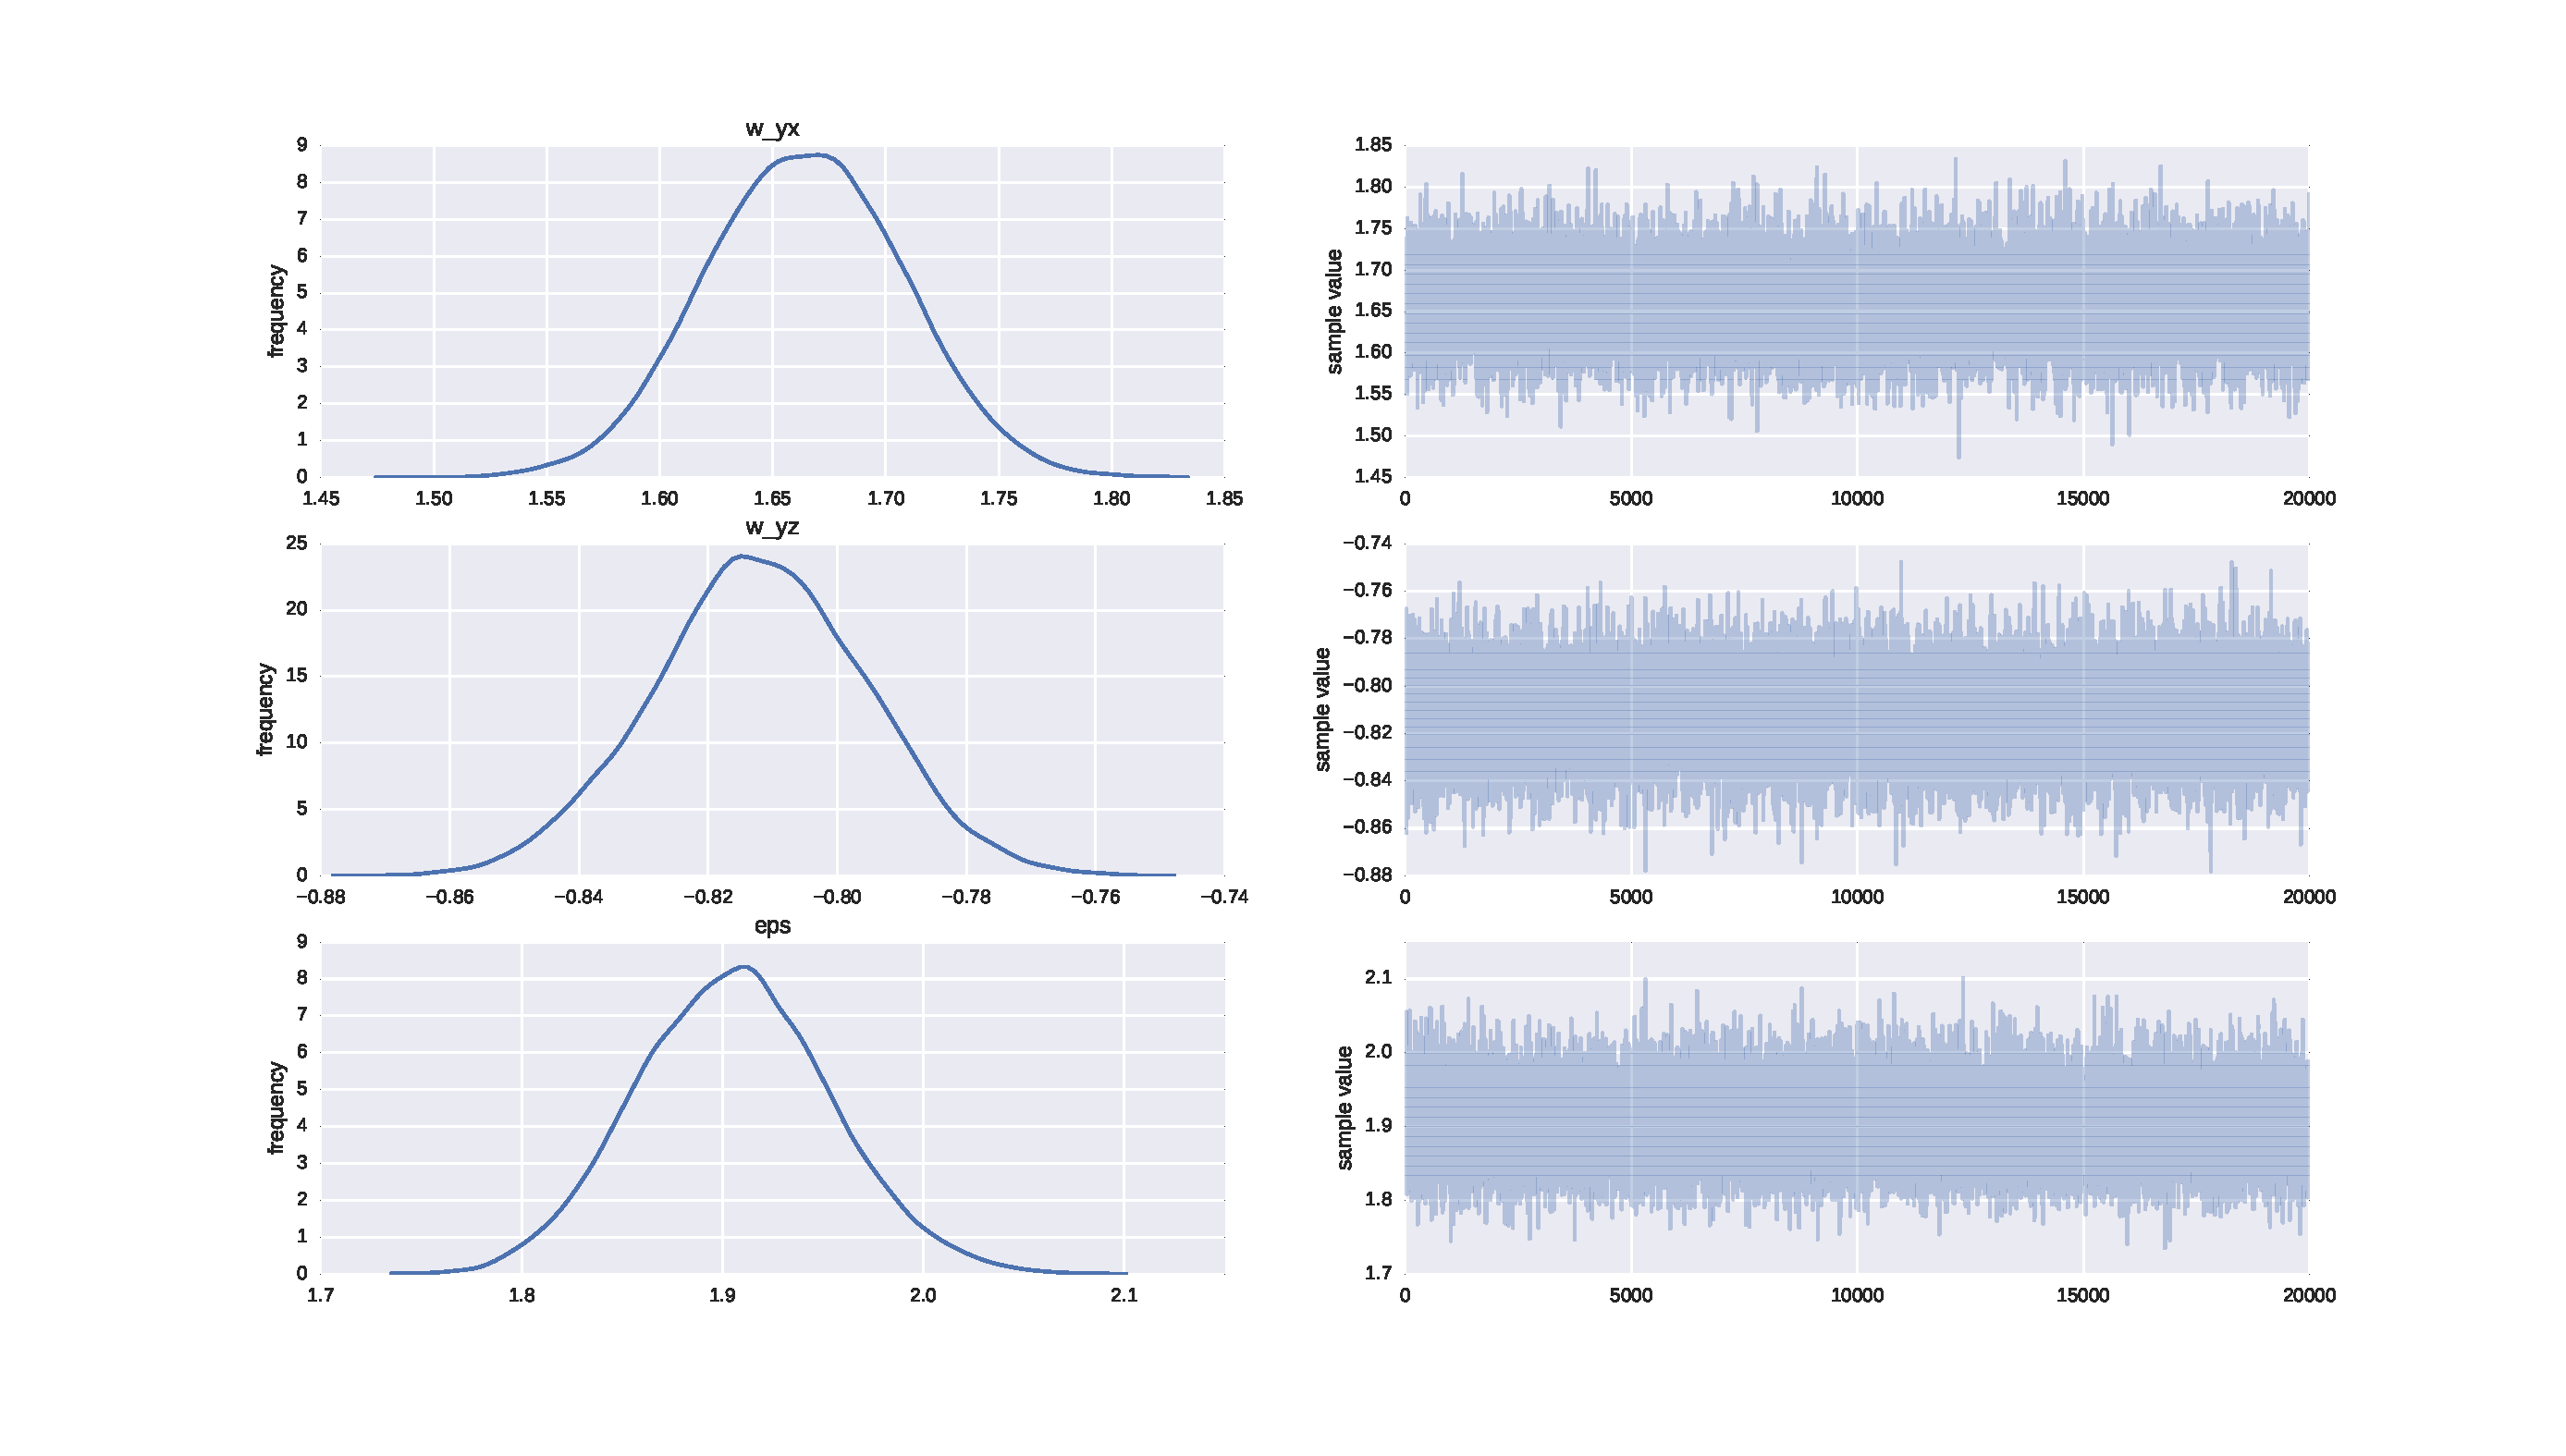
\includegraphics[scale=1]{prior_bad_prior.pdf}
\end{subfigure}
\caption{An example demonstrating how selecting a prior for a nuisance parameter centered around the causal effect of that parameter on the outcome, rather than its association with the outcome, can bias estimates for actual parameter of interest. We sample $n=1000$ data points from the joint distribution defined by $P(U)P(Z|U)P(X|Z)P(Y|U,Z,X) \sim N(0,1)N(2U,0.09)N(0.5Z,1)N(3U -Z + 0.5X , 0.25)$ and fit the model $Y \sim N(w_yx X+\beta Z,\epsilon)$ in Stan and plot the posterior distributions over $w_yx$ and $\beta$. Figure (a) shows the results with no prior (equivalently an improper prior) for both $w_yx$ and $\beta$. Figure (b) shows the results when we place a Gaussian prior centered around the $w_yz$ on the distribution for $\beta$.}\label{fig:careful-prior-example}
\end{figure}

This result is counter intuitive. When fitting a model to estimate the effect of marketing on sales, it is natural to put a prior on the coefficient for price that is strongly negative because we believe increasing price decreases sales. However, our prior should be on the expected association between price and sales, holding fixed all the other variables in the model, not the causal relationship between price and sales. An alternative is to explicitly include $U$ as a latent variable in the model. However, this comes at a computational cost with little benefit for estimation, unless we have good knowledge of the relationships between $U$, $Z$ and $Y$. More fundamentally, at whatever level we decide to stop adding latent variables and specify a prior, we can introduce this form of bias if priors are selected naively on the basis of causal intuition. The issue is not limited to linear-Gaussian models. This is an important insight for the many applications of Bayesian modelling that make use of human-elicited priors, since people tend to think causally. The solutions, either explicitly modelling latent variables to higher levels or allowing for them in setting priors, have the effect of broadening the priors over nuisance parameters in the model. 


\chapter{Learning from interventions}
\label{chap:interventionalist_view}

The previous sections focused on aspects of the problem of estimating the likely effect of an intervention from data gathered prior to making the intervention. There is an obvious alternative. Instead of trying to infer the outcome of an intervention from passive observations, one can intervene and see what happens. There are three key differences between observing a system and explicitly intervening in it. First, we determine the nature of the intervention and thereby control the data points used to estimate causal effects. Selecting data points optimally for learning is the focus of the optimal experimental design literature within statistics \citep{pukelsheim2006optimal} and the active learning literature in machine learning \citep{settles2010active}. Secondly, explicitly choosing interventions yields a perfect model of the probability with which each action is selected, given any context, allowing control over confounding bias. Finally, when we are intervening in a system we typically care about the impact of our actions on the system in addition to optimising learning. For example, in a drug trial , assigning people a sub-optimal treatment has real world costs. This leads to a trade-off between exploiting the best known action so far and exploring alternative actions about which we are less certain. This exploration-exploitation trade-off lies at the heart of the field of reinforcement learning \citep{sutton1998reinforcement}. 

\section{Randomised experiments}
\label{sec:randomized_experiment}
Randomised controlled trials are often presented as the gold standard for determining causal effects. What is it about randomisation that makes it so important when it comes to causality? The graphical model for a randomised controlled experiment is shown in figure \ref{fig:random_experiment_network}. If we assume perfect compliance (everyone takes the treatment that we select for them) then we have a perfect model for the treatment assignment process. Since treatment is assigned randomly, there can be no other variables that influence it and thus no confounding variables that affect both treatment and outcome. 

\begin{figure}
\centering
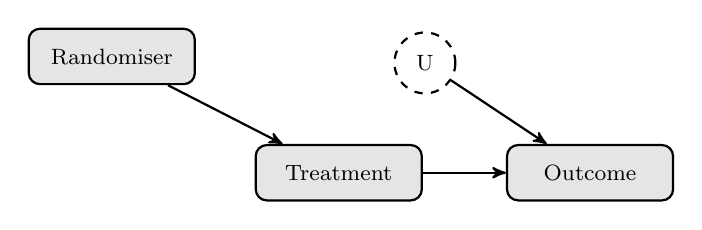
\begin{tikzpicture}[->,shorten >=0pt,shorten <=0pt,node distance=3em,thick, node/.style={observedrect}, lt/.style={latent}]
\node[node](1){Treatment};
\node[node, above left=of 1](2){Randomiser};
\node[node, right=of 1](3){Outcome};
\node[lt, above left=of 3](4){U};
\path[]
	(2) edge (1)
	(1) edge (3)
	(4) edge (3);
\end{tikzpicture}
\caption{causal network for a randomised experiment}
\label{fig:random_experiment_network}
\end{figure} 

Randomisation does not ensure target and control group are exactly alike. The more other features (observed or latent) influence the outcome, the more likely it is that there will be a significant difference in the joint distribution of these variables between the target and control groups in a finite data sample. However, the variance in the outcome, within both the target and control groups, also increases. The net result is increased variance (but not bias) in  the estimate of causal effects. 

Stratified randomised experiments address the issue of variance due to covariate imbalance by randomly allocating treatment conditional on covariates believed to influence the outcome of interest. If we stratify in such a way that the probability an instance receives a given treatment is independent of its covariates, for example, by grouping instances by each assignment to the covariates and then assigning treatment randomly with fixed probabilities, the causal graphical model in figure \ref{fig:random_experiment_network} still holds. We can then estimate the average causal effects directly from the differences in outcome across treatments. More complex stratification strategies can introduce a backdoor path from treatment to outcome via the covariates on which treatment is stratified, (figure \ref{fig:random_experiment_network_stratified}). This necessitates that one condition on these covariates in computing the average casual effect in the same way as for estimating causal effects under under ignorability (\S\ref{sec:causal_effect_under_ignorability}). The key difference is that the propensity score is known, as it is designed by the experimenter, and there are guaranteed (rather than assumed) to be no latent confounding variables (that influence both treatment and outcome). See \citet{imbens2015causal} for a discussion of the trade-offs between stratified versus completely random experiments. 

\begin{figure}
\centering
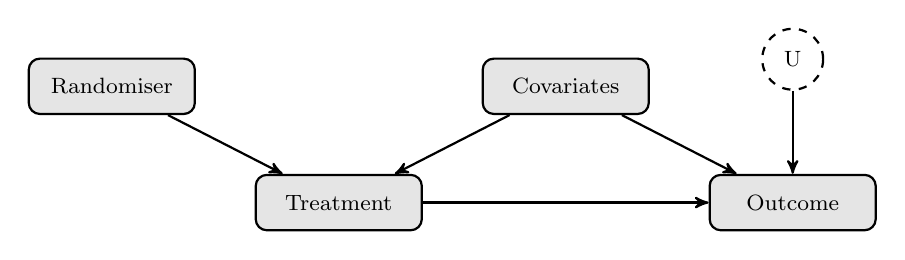
\begin{tikzpicture}[->,shorten >=0pt,shorten <=0pt,node distance=3em,thick, node/.style={observedrect}, lt/.style={latent}]
\node[node](1){Treatment};
\node[node, above left=of 1](2){Randomiser};
\node[node, above right=of 1](5){Covariates};
\node[node, below right=of 5](3){Outcome};
\node[lt, above=of 3](4){U};

\path[]
	(2) edge (1)
	(1) edge (3)
	(4) edge (3)
	(5) edge (3) edge (1);
\end{tikzpicture}
\caption{causal network for a stratified randomised experiment if the probability an individual is assigned a given treatment depends on some covariates.}
\label{fig:random_experiment_network_stratified}
\end{figure} 

The benefit provided by randomisation in breaking the link between the treatment variable and any latent confounders should not be understated. The possibility of unobserved confounders cannot be empirically ruled out from observational data \citep{Pearl2000} (there is no test for confounding). This means causal estimates from non-experimental data are always subject to the criticism that an important confounder may have been overlooked or not properly adjusted for. However, randomised experiments do have some limitations. 

\subsection{Limitations of randomised experiments}
\label{subsec:limitations_of_experiment}

The idealised notion of an experiment represented by figure \ref{fig:random_experiment_network} does not capture the complexities of randomised experiments in practice. There may be imperfect compliance so that the treatment selected by the randomiser is not always followed, or output censoring in which the experimenter is not able to observe the outcome for all units (for example if people drop out). If compliance or attrition is not random, but associated with (potentially latent) variables that also affect the outcome, then the problem of confounding bias returns.\footnote{Non-compliance is a problem if the goal is to estimate the causal effect of the treatment on the outcome but not if the goal is to estimate the causal effect of prescribing the treatment. The latter makes sense in a context where the process by which people decide whether to take the treatment they have been prescribed is likely to be the same if the treatment were made available more generally beyond the experimental trial.} See figure \ref{fig:random_experiment_network_imperfect_compliance} for a graphical model of a randomised experiment with imperfect compliance.

\begin{figure}
\centering
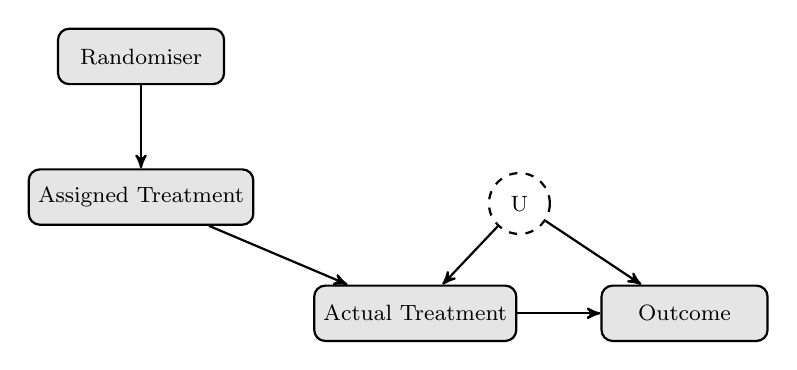
\begin{tikzpicture}[->,shorten >=0pt,shorten <=0pt,node distance=3em,thick, node/.style={observedrect}, lt/.style={latent}]
\node[node](1){Actual Treatment};
\node[node,above left=of 1](5){Assigned Treatment};
\node[node, above =of 5](2){Randomiser};
\node[node, right=of 1](3){Outcome};
\node[lt, above left=of 3](4){U};
\path[]
	(2) edge (5)
	(5) edge (1)
	(1) edge (3)
	(4) edge (3) edge (1);
\end{tikzpicture}
\caption{causal network for a randomised experiment with imperfect compliance}
\label{fig:random_experiment_network_imperfect_compliance}
\end{figure} 

It is not always possible or ethical to conduct a randomised controlled trial, as is beautifully demonstrated by the paper of \citet{smith2003parachute} on randomised cross-over trials of parachute use for the reduction of the mortality and morbidity associated with falls from large heights \ref{fig:parashute}. When experimentation is possible, it is frequently difficult or expensive. This means experimental data sets are often much smaller than observational ones, limiting the complexity of models that can be explored. In addition, they are often conducted on a convenient, but unrepresentative, sample of the broader population of interest (for example first year university students). This can result in estimates with high \emph{internal validity} \citep{Campbell1963}, in that they should replicate well in a similar population, but very low \emph{external validity} in that the results may not carry over to the general population of interest. The question of whether an experiment conducted on one population can be mapped to another is referred to as the transportability problem \citep{Bareinboim2013} and relies on very similar assumptions and arguments to causal inference and the do-calculus. 

\begin{figure}
\begin{center}
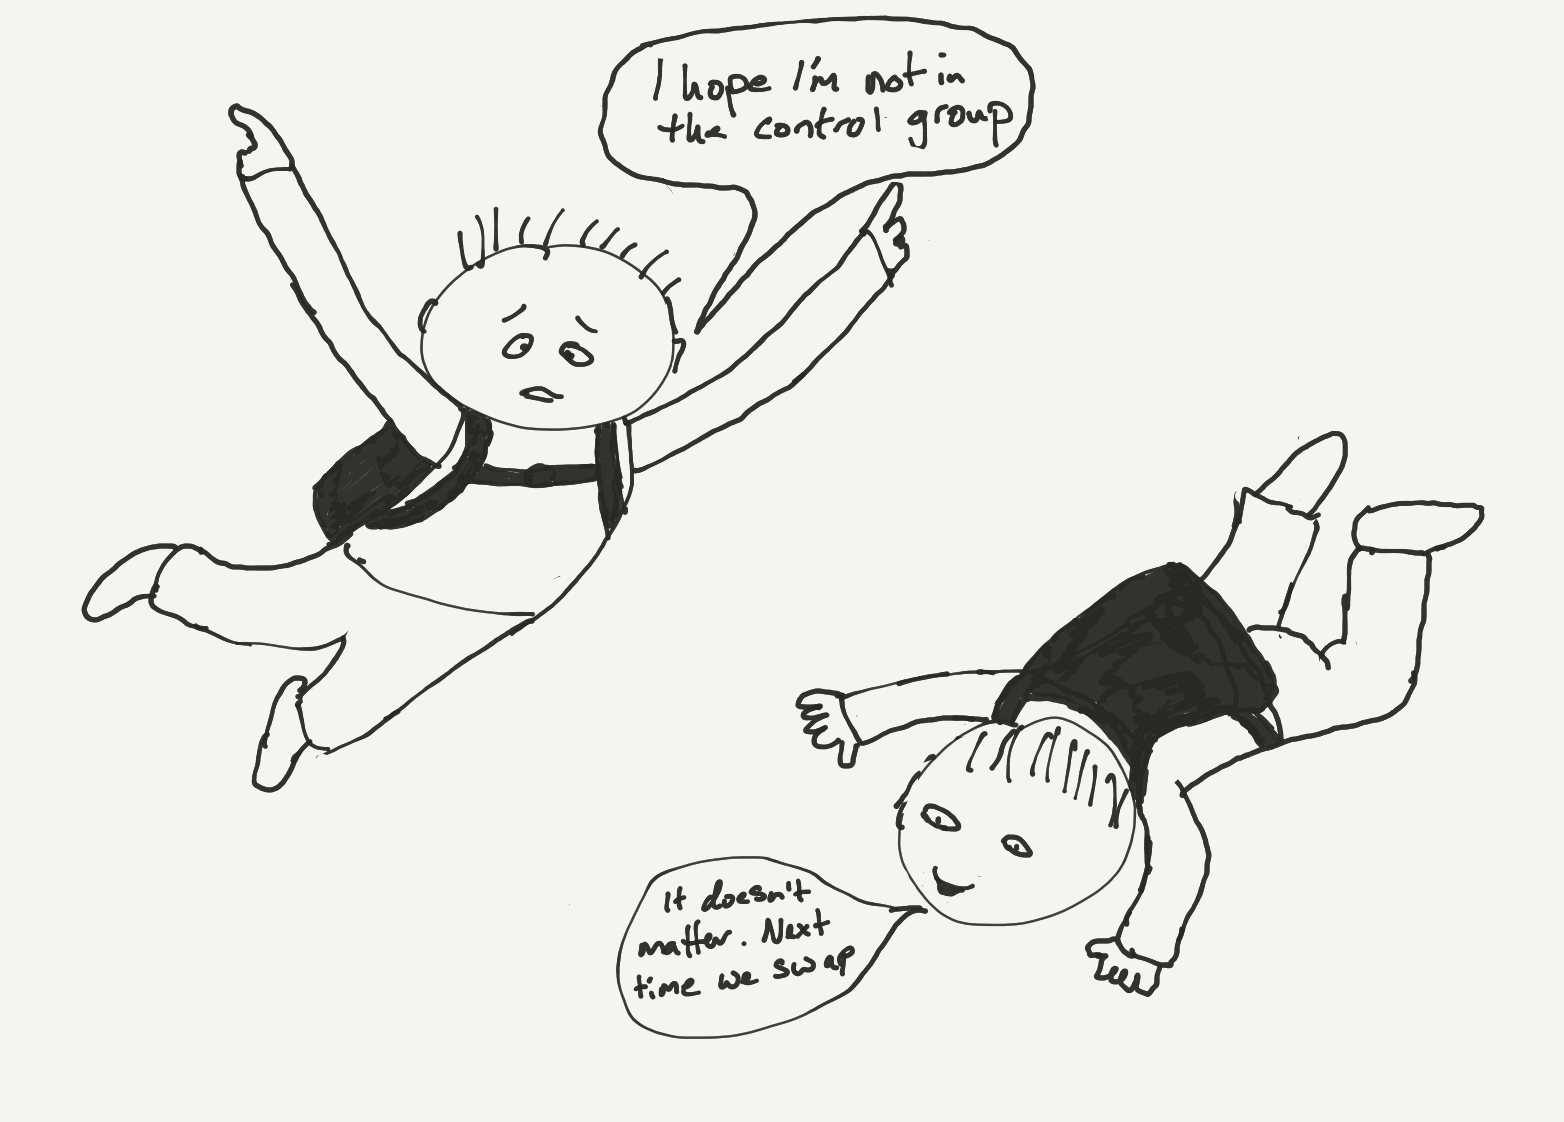
\includegraphics[scale=.4]{double_blind_parashute_trial_cartoon.png}
\end{center}
\caption{Experiments are not always ethical; an illustration of a randomised cross-over trial of parachutes for the prevention of morbidity and mortality associated with falls from large heights.}
\label{fig:parashute}
\end{figure}

Finally, non-adaptive randomised experiments are not optimal from either an active or reinforcement learning perspective. As an experiment proceeds, information is obtained about the expectation and variance of each intervention (or treatment). Fixed experimental designs cannot make use of this information to select which intervention to try next. This results in both poorer estimates for a fixed number of experimental samples and more sub-optimal actions during the course of the experiment.

\section{Multi armed bandits}
\label{sec:multi-armed-bandits}

Multi-armed bandits address the problem of designing experiments that can adapt as samples are observed. Their introduction is generally attributed to \citet{Thompson1993}. In its classic formulation \citep{Robbins1952,Lai1985} the (stochastic) k-armed bandit describes a sequential decision making problem, with $k$ possible actions or arms. Each arm $i$ is associated with a fixed but unknown reward distribution. \footnote{In order to quantify the performance of bandit algorithms, some assumptions are required on the distributions from which the rewards are generated. It sufficient (but not necessary) to assume they are sub-Gaussian.} For each time step up to some horizon $T$, the learner selects an action and receives a reward, sampled i.i.d from the marginal distribution corresponding to that action. The goal of the learner is to maximise the total reward they receive. This problem captures the exploration-exploitation trade-off. The learner must balance playing arms that have yielded good results previously with exploring arms about which they are uncertain.

\vspace{0.5cm}
\begin{definition}[Stochasitic k-armed bandit problem]
Let $\actionspace = \set{1,...,k}$ be the set of available actions (or bandit arms) and $\P{\vec{y}} = \P{\cf{Y}{1},...,\cf{Y}{k}}$ be a joint distribution over the rewards for each action. The multi-armed bandit problem proceeds over $T$ rounds. In each round $t$, 
\begin{enumerate}
\item the learner selects an action $a_{t} \in \set{1,...,k}$, based on the actions and rewards from previous time-steps and a (potentially stochastic) \emph{policy} $\pi$
\item the world stochastically generates the rewards for each action, $[\cfb{Y}{1},...,\cfb{Y}{k}] \sim \P{\vec{y}}$
\item the learner observes and receives (only) the reward for the selected action $\cfb{Y}{a_t}$ 
\end{enumerate}

At the end of the game, the total reward obtained by the learner is $\sum_{t=1}^T \cfb{Y}{a_t}$. We denote the expected reward for the action $i$ by $\mu_i$ and the action with the highest expected reward by $i^*$. Note we have used counterfactual notation (see section \ref{sec:counterfactuals}) to denote the rewards for each action, $\cfb{Y}{i}$ is the reward the algorithm would have received had it selected action $i$ at timestep $t$. I discuss the (potentially) counterfactual nature of regret further in section \ref{sec:counterfactual-nature-regret}.
\end{definition} 


The total reward a bandit algorithm/policy can expect to achieve depends on the distributions from which the rewards for each action are sampled. To account for this, the performance of bandit algorithms is quantified by the difference between the reward obtained by the algorithm and the reward that would have been obtained by an oracle that selects the arm with the highest expected reward at every time step. This difference is known as the (cumulative) regret \footnote{The term regret is somewhat overloaded in the reinforcement learning literature. There are alternative definitions that arise in the related problems of adversarial bandits and learning from expert advice. In addition, researches often refer to the expected regret as \quotes{the regret}.}.
\eqn{
\label{eqn:raw_regret}
\rawregret = \sum_{t=1}^T \cfb{Y}{i^*} - \sum_{t=1}^T \cfb{Y}{a_t}
}

Both the rewards and the actions selected by the algorithm are random variables. The majority of work in the bandit literature focuses on analysing and optimising some form of the expected regret, however there has been some work that also considers the concentration of the regret \citep{Auer1995,Audibert2007,Audibert2009exploration}. The expectation of the regret, as defined by equation \ref{eqn:raw_regret}, is referred to as the pseudo-regret \citep{Bubeck2012} and is given by equation \ref{eqn:pseudo_regret}. A stochastic bandit algorithm is learning if it obtains pseudo-regret that is sub-linear in $T$. 

\vspace{0.5cm}
\begin{definition}[Pseudo-Regret]
\eqn{
\label{eqn:pseudo_regret}
\regret(\pi) &= \max_{i \in \set{1,...,k}}\E{\sum_{t=1}^T{\cfb{Y}{i}}} - \E{\sum_{t=1}^T{\cfb{Y}{a_t}}} \\
&= T\mu_{i^*} - \E{\sum_{t=1}^T{\cfb{Y}{a_t}}}
}
\end{definition}

The regret is invariant to adding a constant to the expected rewards for all actions. However, it still depends on key characteristics of the reward distributions for each action. Bandit algorithms are designed given assumptions about the form of the distributions, such as that they come from a given family (i.e Bernoulli bandits, Gaussian bandits), or that the rewards are bounded in some range. Given these assumptions, the performance of the algorithm is characterised in two ways; by the \emph{problem-dependent regret}, which typically depends on how far each arm is from optimal and by the \emph{worst case regret}, which is the maximum regret over all possible configurations of the reward distributions (for a given horizon $T$ and number of arms $k$).

\subsection{Stochastic bandits: Approaches and results}
\label{sec:stochastic-bandit}

The adaptive nature of multi-armed bandit algorithms complicates the design and analyse of estimators. The action selected by an algorithm at a given timestep can depend on the history of previous actions and rewards. As a result, the probability that each action is selected evolves over time, the actions are not sampled i.i.d from a fixed distribution and the number of times each action is selected is a random variable. The expectation and variance guarantees of standard estimators do not hold in this setting (see figure \ref{fig:early_stopping} for a concrete example). This makes it very difficult to  obtain an analytical expression for the expected regret for a given algorithm and problem. Instead, the focus is on computing bounds on the expected regret. 

\begin{figure}[h]
\centering
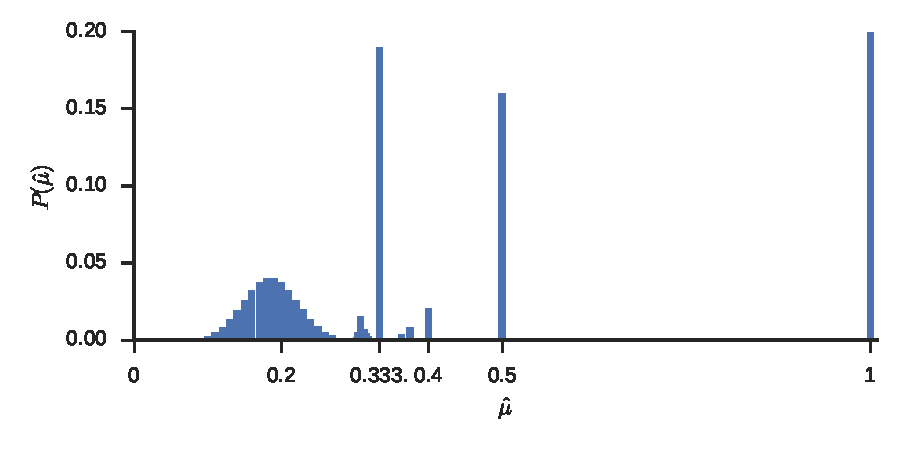
\includegraphics[scale=1]{extreme_early_stopping}
\caption{Standard empirical estimators can be biased if the number of samples, $n$, is not fixed in advance, but is a random variable that depends on the values of previous samples. This example plots the distribution (over $10^6$ simulations) of $\hat{\mu} = \frac{1}{n}\sum_{i=1}^n X_i$, where $X_i \sim Bernoulli(0.2)$. In each simulation, we stop taking samples if the average value of $X_i$ up to that point exceeds a threshold of $0.3$ or $n$ reaches $100$. $\E{\hat{\mu}} = 0.439$. The estimator is substantially biased above $\E{X_i} = 0.2$ by the early stopping. Note that excluding experiments that were stopped early creates a bias in the opposite direction, $\E{\hat{\mu}|n=100} = 0.185$, as trials that obtained positive results early are excluded. This has some interesting real world implications. Early stopping of clinical trials is controversial. A researcher conducting a meta-analysis who wished to avoid (rather than bound) bias due to early stopping would have to exclude not only those trials which were stopped early but those which \emph{could} have been stopped early.}
\label{fig:early_stopping}
\end{figure}

There are a few key principles that are used to guide the development of bandit algorithms. The simplest is to explicitly separate exploration from exploitation, and base estimation of the expected rewards of each arm only on the data generated during exploration steps. A common example in practice is uniform exploration (or A/B testing) for some fixed period followed by selecting the action found to be best during the exploration phase. This results in simpler analysis, particularly if the number of exploration steps is fixed in advance, however it is sub-optimal, even if the exploration period is adaptive \citep{NIPS2016_6179}. 

Another key approach is \emph{optimism in the face of uncertainty}. Applied to stochastic bandits, the optimism in the face of uncertainty principle suggests computing a plausible upper bound for the expected reward of each arm, and selecting the arm with the highest upper bound. The optimism principle encourages exploitation and exploration because a high upper bound on the expected reward for an action implies either the expected reward or the uncertainty about the reward for that action is high. Thus selecting it yields either a good reward or useful information. 

\citet{Lai1985} leveraged the optimism in the face of uncertainty principle to develop an algorithm for specific families of reward distributions, including the exponential family. They showed that, for a given bandit problem, the pseudo-regret increased with $\bigo{log(T)}$ asymptotically and proved this is asymptotically efficient. However, their algorithm is complex and memory intensive to compute as, at each timestep, it relies on the entire sequence of rewards for each arm. \citet{Agrawal1995} developed a simpler algorithm that computed upper bounds based only on the mean of previous samples for each arm, whist retaining the logarithmic dependence on $T$. Finally, \citet{Auer2002} developed the UCB-1 algorithm, see algorithm \ref{alg:ucb-1}, which requires only that the reward distributions are bounded, and proved finite-time regret bounds. We now assume the rewards are bounded in $[0,1]$. The algorithm and regret bounds can be generalised to submission reward distributions, see \citet{Bubeck2012}.

\begin{algorithm}[H]
\caption{UCB-1}\label{alg:ucb-1}
\begin{algorithmic}[1]
\STATE {\bf Input:} horizon $T$.
\STATE Play each arm once. 
\FOR{$t \in 1,\ldots,T$}
\STATE Count the number of times each arm has been selected previously $n_{t,i} = \sum_{s=1}^{t-1} \ind{a_s = i}$
\STATE Calculate the mean reward for each arm $\hat{\mu}_{t,i} = \frac{1}{n_{t,i}} \sum_{s=1}^{t-1}\ind{a_s = i}Y_t$
\STATE Select arm $a_t \in \argmax_{i = \set{1,...,k}}\left(\hat{\mu}_{t,i}+\sqrt{\frac{2 \log{t}}{n_{t,i}}}\right)$
\ENDFOR
\end{algorithmic}
\end{algorithm}
 
Let $\Delta_i = \mu_i - \mu^*$ be degree to which each arm is sub-optimal. The problem-dependent pseudo-regret for UCB-1 is bounded by equation \ref{eqn:ucb_problem_dependent_regret} \citep{Bubeck2012},

\eqn {
\label{eqn:ucb_problem_dependent_regret}
\regret \leq & \sum_{i:\Delta_i > 0}\left(\frac{8\log(T)}{\Delta_i}+2 \right)
}

Somewhat unintuitively, the regret increases as the value of the arms gets closer together. This is because it becomes harder for the algorithm to identify the optimal arm. As the differences $\Delta_i \rightarrow 0$, the regret bound in \ref{eqn:ucb_problem_dependent_regret} blows up, however the regret itself does not - since although we may not be able to distinguish arms with very small $\Delta_i$ from the optimal arm, we also do not lose much by selecting them. The worst case occurs if all arms have the same expected reward $\mu$ except for the optimal arm which has reward $\mu^*=\mu+\Delta$, where $\Delta$ is just too small for the algorithm to learn to identify which arm is optimal given the horizon $T$. The regret cannot exceed what would be obtained by selecting the a sub-optimal arm in every timestep, $T\Delta$, so the worst case regret is bounded by the minimum of equation \ref{eqn:ucb_problem_dependent_regret} and $T\Delta$ which is maximised when they are equal, see figure \ref{fig:ucb_regret_vs_delta}. By solving this equality for $\Delta$ one can show the worst case regret is bounded by equation \ref{eqn:ucb_worst_case_regret}, see \citet{Bubeck2012}.

\eqn{
\label{eqn:ucb_worst_case_regret}
\regret \in \bigo{\sqrt{kT\log(T)}}
}  

\begin{figure}
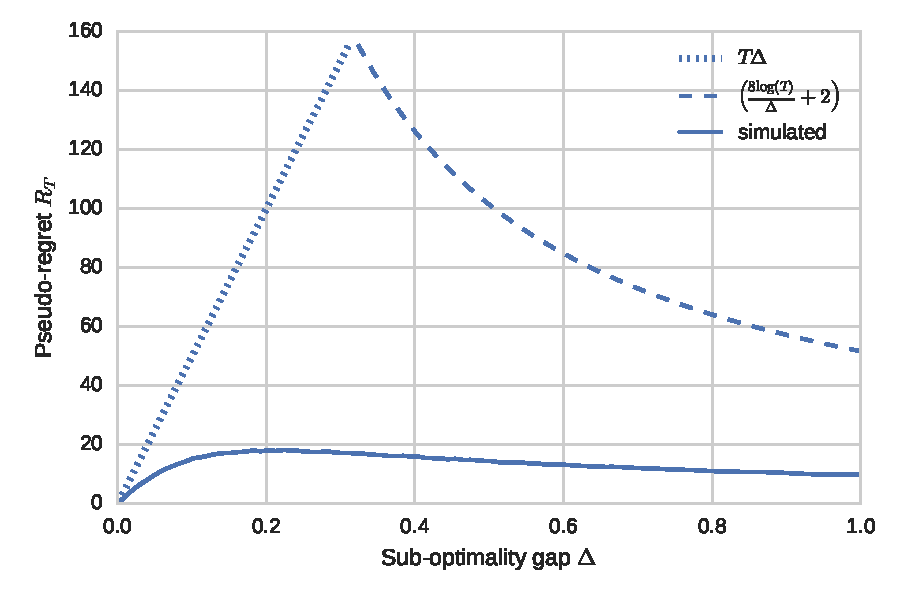
\includegraphics[scale=1]{ucb_regret_vs_delta}
\caption{The regret bound in equation \ref{eqn:ucb_problem_dependent_regret} grows as the differences between the expected rewards for each arm shrink. The solid curve shows the mean (cumulative) regret, over a 1000 simulations for a 2-armed, Bernoulli bandit with fixed horizon, $T = 500$, as a function of the difference in the expected reward for the arms $\Delta$. The dashed curves show the corresponding upper bounds; $T\Delta$ and equation \ref{eqn:ucb_problem_dependent_regret}}
\label{fig:ucb_regret_vs_delta}
\end{figure}

The form of the dependence on the number of arms $k$ and horizon $T$ differs between the problem-dependent and worst case regret. The problem-dependent regret grows linearly with the number of arms, $k$, and logarithmically with $T$. The difference stems from the fact the problem-dependent regret defines how the regret grows for a given set of reward distributions as $T$ increases, whereas in the worst case regret, the gap between expected rewards is varied as a function of $T$. \citet{Auer1995} show that the worst case regret for the k-armed bandit problem is lower bounded by $\regret \in \bigomega{\sqrt{kT}}$

Subtle modifications to the UCB algorithm can eliminate the logarithmic term equation \ref{eqn:ucb_worst_case_regret}. This yields regret $ \bigo{\sqrt{TK}}$ and closes the gap with the worst case lower bound \citep{Audibert2009,Lattimore2015}, whilst retaining a good problem-dependent bound of the form achieved by UCB \citep{Lattimore2015}.

\begin{figure}
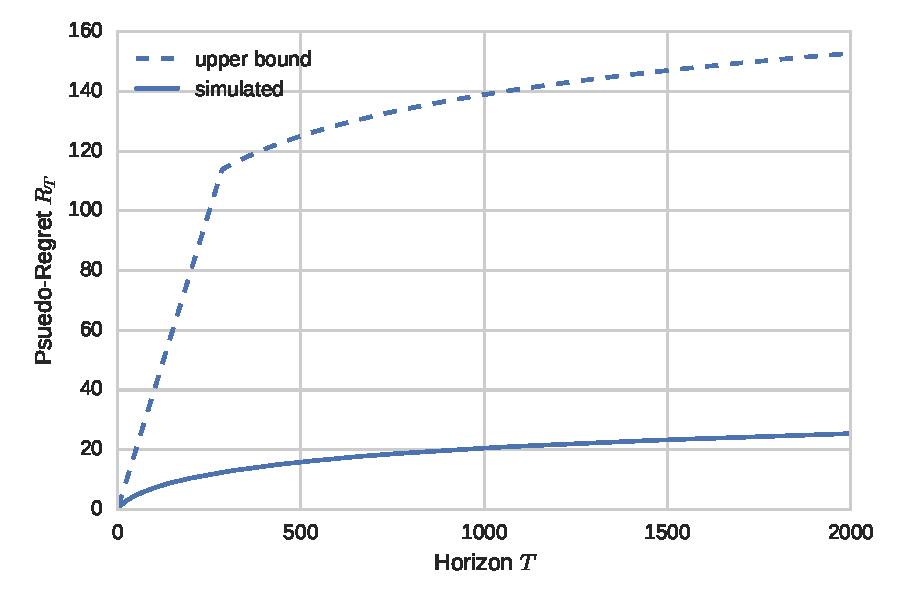
\includegraphics[scale=1]{upper_bound_vs_actual_average_regret}
\caption{The actual performance of the UCB algorithm can be substantially better than suggested by the upper bound, particularly for small $T$. The solid curve shows the mean expected regret associated with the sequence of arms chosen by UCB-1 with $k=2$ arms and the rewards sampled from $bernoulli([.3,.7])$ over 1000 simulations. The dashed curve shows the corresponding upper bound given by the minimum of $T\Delta_{max}$ and equation\ref{eqn:ucb_problem_dependent_regret}.}
\label{fig:ucb_upperbound_vs_actual_performance}
\end{figure}

Finally, there is the heuristic principle of playing each arm with probability proportional to the likelihood that it is optimal. This approach is generally called Thompson sampling as it was the method proposed in the original bandit paper by \citet{Thompson1993}. Thompson sampling has strong empirical performance, \citep{chapelle2011empirical}. However, it is complex to analyse. \citet{kaufmann2012thompson} demonstrate that it obtains optimal problem-dependent bounds, \citet{agrawal2013further} show that it obtains worst case regret of $\bigo{\sqrt{kT\log(T)}}$, equivalent to UCB. 

\subsection{Pure-exploration problems}
\label{sec:pure-exploitation-problems}
Another problem that has attracted recent attention \citep{Bubeck2009,Audibert2010,Gabillon2012,Karnin2013} within the stochastic multi-armed bandit framework is \textit{pure exploration} or \textit{best arm identification}. In this setting, the horizon $T$ represents a fixed budget for exploration after which the algorithm outputs a single best arm $i$. The performance of the algorithm is measured by the simple regret; the expected difference between the mean reward of the (truly) optimal arm and the mean reward of the arm selected by the algorithm.

\vspace{0.5cm}
\begin{definition}[Simple Regret]
\eqn{
\label{eqn:simple_regret}
\simpleregret=\mu_{i^*} - \E{\mu_{\hat i^*}}.
}
\end{definition}

The best arm identification problem arises naturally in applications where there is a testing or evaluation phase, during which regret is not incurred, followed by a commercialisation or exploitation phase. For example, many strategies might be assessed via simulation prior to one being selected and deployed. The worst case simple regret for a k-armed bandit is lower bounded by equation \ref{eqn:worst_case_simple_regret_lower_bound} (\citep{Bubeck2009}).

\eqn{
\label{eqn:worst_case_simple_regret_lower_bound}
\simpleregret \in \bigo{\sqrt{K/T}}
}


%\todo{discuss the key ways in which the simple regret problem differs from cummulative regret}

Pure-exploration does not mean simply playing the arm with the widest uncertainty bounds. The goal is to be sure the arm we believe is optimal is in fact optimal at the end of the exploration period. 

\subsection{Adversarial Bandits}
\label{sec:adversarial-bandits}

Adversarial bandits, described by \citet{Auer1995}, are an alternate, widely studied, setting that relaxes the assumption that rewards are generated stochastically. Instead, simultaneously with the learner selecting an action $a_t$, a potentially malicious adversary selects the reward vector $\boldsymbol{Y}_t$. As in the stochastic setting, the learner then receives reward only for the selected action. 

\vspace{0.5cm}
\begin{definition}[Adversarial k-armed bandit problem]
\label{def:adversarial-k-armed-bandit}
Let $\actionspace = \set{1,...k}$ be the set of available actions.  In each round $t \in 1,...,T$, 
\begin{enumerate}
\item the world (or adversary) generates, but does not reveal, a vector or rewards $\vec{Y_t}=[\cfb{Y}{1},...,\cfb{Y}{k}]$. 
\item the learner selects an action $a_{t} \in \set{1,...,k}$, based on the actions and rewards from previous time-steps and a (potentially stochastic) \emph{policy} $\pi$
\item the learner observes and receives (only) the reward for the selected action $\cfb{Y}{a_t}$ 
\end{enumerate} 
\end{definition}

Adversaries that generate rewards independently of the sequence of actions selected by the learner in previous time steps are referred to as \emph{oblivious}, as opposed to \emph{non-oblivious} adversaries, which can generate rewards as a function of the history of the game. In the case of oblivious adversaries, we can also define the adversarial bandit problem by assuming the adversary generates the entire sequence of reward vectors before the game commences. 

For oblivious adversarial bandits, we can define regret analogously to stochastic bandits as the difference between the reward obtained by playing the single arm with the highest reward in every round and the expected reward obtained by the algorithm \footnote{This is also referred to as the weak regret, since in the adversarial case, it can make more sense to compare against the best sequence of arms rather than the best single arm.}. We do not have to take the expectation over the first term of equation \ref{eqn:pseudo_regret-adversarial} because the sequence of rewards is fixed. However the reward obtained by the algorithm is still a random variable as we are considering randomised algorithms.  

\eqn{
\label{eqn:pseudo_regret-adversarial}
\regret(\pi) &= \max_{i \in \set{1,...,k}}{\sum_{t=1}^T{\cfb{Y}{i}}} - \E{\sum_{t=1}^T{\cfb{Y}{a_t}}}
}

The policy (or algorithm) used by the learner is available to the adversary before the game begins, and there are no limitations placed on the amount of computation the adversary can perform in selecting the reward sequences. This implies the adversary can ensure that any learner with a deterministic policy suffers regret $\bigo{T}$ by forecasting their entire sequence of actions. For example, if the learner will play $a_1 = 1$ in the first round, then the adversary sets the reward $\vec{Y_1} = [0,1,1,...1]$, forecasts what action the learner will play in round 2, given they received a reward of 0 in round 1, and again generates the reward vector such that the action the learner will select obtains no reward, and all other actions obtain the maximum reward. This implies adversarial bandit policies must be sufficiently random to avoid such exploitation \footnote{The UCB algorithm, defined by algorithm \ref{alg:ucb-1}, is deterministic if the order in which arms are played during the first $k$ rounds is fixed and the method for selecting which arm to play when multiple-arms have the same upper-confidence bound is not-random (for example, select the arm one with the lowest index $i$).}

The seminal algorithm for adversarial bandits is Exp-3 \citep{Auer2002}, which, like UCB, obtains worst case pseudo-regret of $\bigo{\sqrt{TK\log(T)}}$  \citep{Auer1995}. Optimal algorithms, with $\regret = \bigo{\sqrt{TK}}$, have also been demonstrated for the oblivious adversarial setting \citep{Audibert2009}. The focus, for adversarial bandits, is on analysing the worst case regret because the problem-dependent regret is not well defined without additional assumptions. However, there has been recent work on developing algorithms that are optimised for both the adversarial and stochastic settings, in that they are sufficiently cautious to avoid linear regret in the adversarial setting, but can nonetheless obtain good problem-dependent regret in more favourable environments \citep{bubeck2012bothworlds,Auer2016}. 

Adversarial bandits appear to be more applicable to real world problems because they do not assume that the rewards associated with each arm are constant over time or independent of the previous actions of the learner. However, pseudo-regret, as defined in equation \ref{eqn:pseudo_regret-adversarial}, does not fully capture an algorithms performance in such cases because it is defined with respect to playing the single arm with the best average return over the game. In settings where the rewards change over time, the pseudo-regret can be negative (see figure \ref{fig:non-stationary-bandit}) so upper bounds on the pseudo-regret do not reflect how sub-optimal the algorithm may be. An example of a setting that lies between stochastic and adversarial bandit problems is the non-stationary setting, in which the rewards are generated stochastically from a distribution that varies over time. Adversarial bandit algorithms may perform better in such settings than standard stochastic policies to the extent that they explore more (to avoid the adversary simulating their behaviour) and thus adapt quicker to changes in the reward distribution. Adversarial algorithms also have stronger worst case regret guarantees, since even the weak regret for stochastic bandits is not guaranteed to be sub-linear in such settings. However, if there are constraints on how rapidly or frequently the reward distributions can change over time, it is better to use algorithms specifically developed to exploit such information and compare them against a stronger notion of regret (see for example \citep{garivier2008upper,Garivier2011a,Besbes2014}). 

\begin{figure}[h]
    \begin{subfigure}[t]{0.49\textwidth}
	\centering   
	 \caption{Behaviour over time}\label{fig:non-stationary-bandit-time} 
         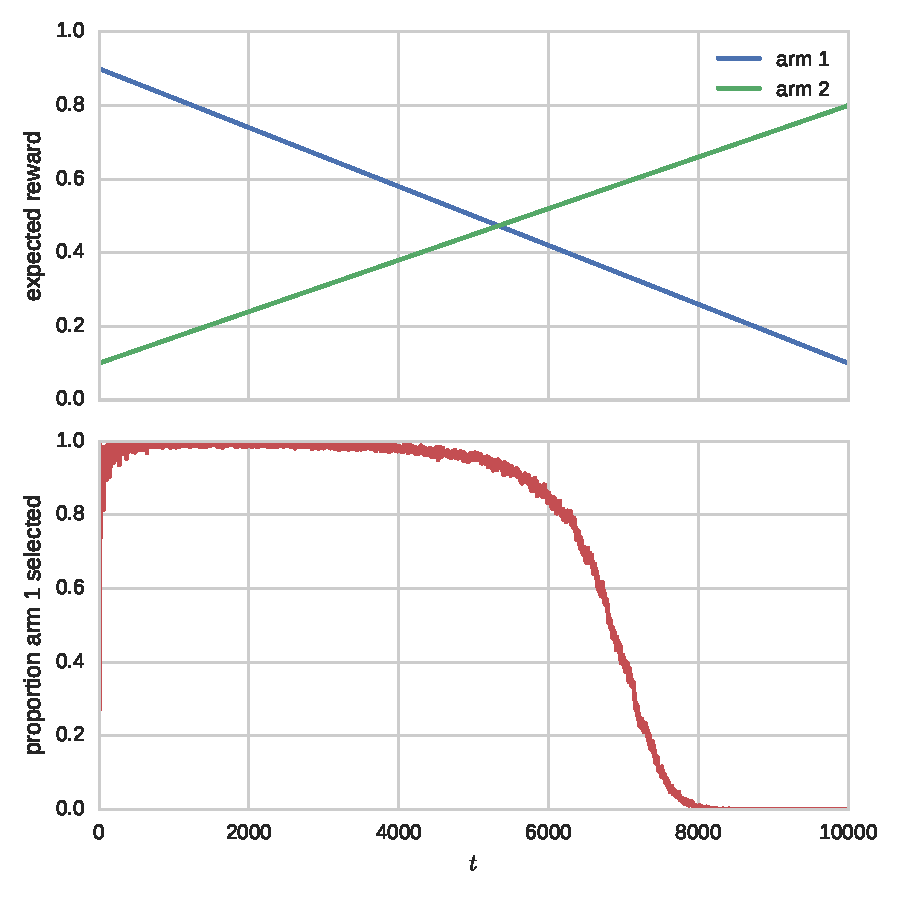
\includegraphics[scale=.5]{non-stationary-bandit-time}
\end{subfigure}
    \begin{subfigure}[t]{0.49\textwidth}
    \centering
     \caption{Cumulative regret distribution}
        \label{fig:non-stationary-bandit-regret}
        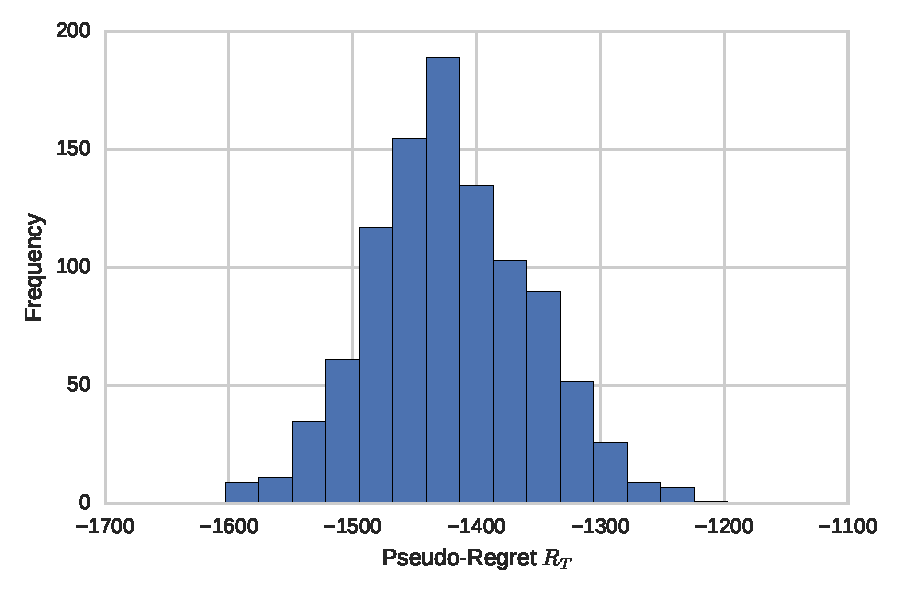
\includegraphics[scale=.5]{non-stationary-bandit-regret}
    \end{subfigure}
      \caption{The pseudo-regret can be negative if rewards are non-stationary. This example shows the results of 1000 simulations of running the UCB-1 algorithm on a 2-armed Bernoulli bandit problem where the expected rewards change linearly over time, up to a horizon $T=10,000$. Figure (a) shows the expected rewards of each arm, and the proportion of time that arm-1 is played, as a function of time. The single best-arm is arm-1 as it has the highest expected reward (averaged over $t$). An oracle that selects arm-1 in every round obtains an expected reward of $5,000$. However, despite not being designed to do so, the UCB-algorithm can adapt to the changing reward distribution to obtain consistently higher rewards. The distribution of regret over the 1000 simulations is shown in figure (b).}\label{fig:non-stationary-bandit}
\end{figure}

\subsection{Contextual bandits}
\label{sec:contextual-bandits}

In the standard multi-armed bandit setting, each decision is identical and the goal is to learn a single best action. However, in most real life (sequential) decision making processes, the optimal action depends on some context. The best treatment to offer an individual patient could depend on their age, gender, disease sub-type or genetics and will not always align with the treatment that is best on average (or for the majority of people).  Similarly, decisions on which ad or content to display on a webpage, or which product to recommend, can be \emph{personalised} based on the previous behaviour of the user. A movie recommender system that learned a single \quotes{best} movie for everyone would not be very useful. 

Contextual bandits are a generalisation of multi-armed bandits that make use of this additional contextual information. The term contextual bandit was coined by \citet{Langford2008}. However, close variants of the underlying problem have also been posed under the names; \quotes{associative reinforcement learning} \citep{kaelbling1994associative}, \quotes{bandits with concomitant variables}\citep{woodroofe1979one} and  \quotes{bandit problems with side information} \citep{wang2005bandit}. 

\vspace{0.5cm}
\begin{definition}[Stochastic Contextual Bandit \footnote{Contextual bandits can also be defined in the adversarial setting analogously to definition \ref{def:adversarial-k-armed-bandit}}]
\label{def:contextual-bandit-problem}
Let $\P{\vec{x},\vec{y}}$ be the joint distribution over the rewards for each action and some context $\vec{X} \in \mathcal{X}$. In each round $t \in \set{1,...T}$, 
\begin{enumerate}
\item the world stochastically generates the vector of rewards for each action and the context, $(\vec{X}_t,[\cfb{Y}{1},...,\cfb{Y}{k}]) \sim \P{\vec{x},\vec{y}}$ and reveals $\vec{X}_t$ to the learner
\item the learner selects an action $A_{t} \in \set{1,...,k}$, based on the context as well as actions and rewards from previous time-steps,
\item the learner observes and receives (only) the reward for the selected action $Y_t = \cfb{Y}{A_t}$ 
\end{enumerate}
\end{definition} 

Standard multi-armed bandits learn to select the action $a$ that, with high probability, maximises $\E{Y|a}$. Contextual bandits learn to select actions that maximise $\E{Y|\vec{x},a}$. The reward for contextual bandits should  be compared to an oracle that acts optimally based on the context. To achieve this, even when the context is continuous, the regret is defined with respect to a class of hypothesis that map from context to action, $h \in \mathcal{H}: \mathcal{X} \rightarrow \set{1,...,k}$. The pseudo-regret is the difference between the expected regret obtained by an oracle that selects actions based on the single best hypothesis or policy $h$ at each timestep, and the expected reward obtained by the algorithm. 

\eqn{
\label{eqn:regret_contextual}
\regret = \max_{h \in \mathcal{H}}\E{\sum_{t=1}^T{\cfb{Y}{h(\vec{X}_t)}}} - \E{\sum_{t=1}^T{\cfb{Y}{A_t}}}
}

If the context is discrete, $\mathcal{X} = \set{1,...,N}$, the contextual bandit problem can be reduced to the standard multi-armed bandit problem by creating a separate standard bandit instance for each value of the context. This approach results in a worst case regret of $\bigo{\sqrt{NkT}}$, with respect to the hypothesis class $\mathcal{H} = \mathcal{X} \times \actionspace$, consisting of all possible mappings from context to action\footnote{This follows from the fact that we have $N$ standard bandit instances, each suffering regret $\bigo{\sqrt{kT_c}}$, where $T_c$ is the number of times context $c$ occurred such that $\sum_{c=1}^N T_c = T$. The regret is maximised if $T_c = T/N$ resulting in total regret $\bigo{N\sqrt{kT/N}}$.}. This is optimal with respect to this class of hypothesis. However, as this reduction treats the problem of learning the correct action for each context completely independently, it cannot leverage any structure in the relationships between different contexts and actions. As in the supervised learning setting, the existence of some form of low-dimensional structure is key to learning in realistic problems, where the context is continuous or high-dimensional \footnote{Even if the context is genuinely discrete, $N$ grows exponentially with the number of variables. For example, with $n$ binary variables, $N = 2^n$}. We expect some form of smoothness; that is, values of context that are similar should lead to comparable rewards for a given action. We need algorithms that can leverage such assumptions. 

An alternate reduction to the standard bandit problem, which allows us to constrain the hypothesis space to explore, is to treat each hypothesis $h$ as a bandit arm \citep{Langford2008}. At each time-step, we select $h \in \mathcal{H}$ based on the rewards previously observed for each hypothesis, take action $h(\vec{x})$ and observe the associated reward. Although this approach removes the explicit dependence on the size of the context, the regret  grows linearly with the size of the hypothesis class considered, limiting our ability to learn any complex mappings from context to actions. The key problem with this approach is each sample is used to update our knowledge about only one hypothesis, as opposed to the supervised learning setting, where each data point is (implicitly) used to compute the loss for every hypothesis simultaneously. 

Suppose that, at each timestep $t$, after selecting an action, the learner received the reward for chosen action but observed the full vector of rewards $[\cfb{Y}{1},...,\cfb{Y}{k}]$. This is known as the full information setting. In this case, the learner can simulate running each hypothesis over the history to compute the reward it would have obtained and use the hypothesis with the best empirical reward to select the next action. This is the \emph{follow the leader} algorithm, which obtains optimal regret $\bigo{\sqrt{T log(\card{\mathcal{H}})}}$ for the full-information problem \citep{cesa2006prediction}. Unfortunately, in the contextual bandit problem, the (counterfactual) rewards associated with alternate action choices are not observed. As in causal effect estimation, we can view this as a missing data problem. However, the data is missing not at random because the component of the reward that is observed depends on the action selected, which in turn is a function of the previous history of actions and rewards. 

The Epoch-greedy algorithm, \citep{Langford2008}, addresses these issues by transforming the contextual bandit problem into a \quotes{data missing at random} problem by explicitly separating exploration from exploitation. Epoch-greedy is an explore-exploit algorithm. It selects actions uniformly at random during an exploration phase and leverages this data to estimate the value of each hypothesis, using inverse propensity weighted estimators to \quotes{fill in} the missing data. The hypothesis with the highest empirical reward is then used to select actions for the remaining time steps. The epsilon-greedy algorithm obtains worst case regret $\bigo{T^{\frac{2}{3}}(k \log{\card{\mathcal{H}}})^{\frac{1}{3}}}$, which has sub-optimal dependence on the horizon $T$.

The Exp-4 algorithm, developed in the context of learning from expert advice (each $h \in \mathcal{H}$ can be viewed as an expert who recommends which action to take), achieves optimal worst case regret of $\bigo{\sqrt{kT log(\card{\mathcal{H}})}}$ in both the stochastic and adversarial settings \citep{Auer2002a}. However, it involves maintaining a list of weights for each hypothesis $h$, resulting in time and memory requirements that grow linearly with the size of the hypothesis space and, unlike the epoch-greedy algorithm, it cannot be generalised to infinite dimensional hypothesis spaces in a straightforward way. The ILOVECONBANDITS algorithm combines the best of both worlds to obtain a computationally efficient algorithm with (almost) optimal regret \citep{Agarwal2014}

Both Epoch-greedy and ILOVECONBANDITS involve solving problems of the form,

\eqn{
\argmax_{h \in \mathcal{H}} \sum_{t=1}^\tau Y_t \ind{h(\vec{X}_t) = A_t}
}

This expression equates to identifying the empirically best policy based on previous data. The algorithms assume the existence of an oracle that can solve this problem and report complexity in terms of the number of calls required to the oracle. The computational tractability of these algorithms on large (or infinite) hypothesis spaces stems from the fact that this problem (also known as the argmax-oracle), can be reduced to solving a cost sensitive classification problem \citep{Dudik2011a}. 

Finally, if we have a parametric model for the relationship between context, action and reward that allows (efficient) computation of the posterior or confidence bounds on the reward for each arm given context, we can develop generalised versions of the UCB or Thompson sampling algorithms. For linear pay-off models, both approaches yield algorithms with strong regret guarantees, \emph{Lin-UCB} \citep{li2010contextual} and \emph{Generalised Thompson Sampling} \citep{Agrawal2013}. 

\subsubsection{The causal structure of contextual bandits}
\label{sec:causal-structure-contextual-bandit}

The definition \ref{def:contextual-bandit-problem} does not make any assumptions about the \emph{causal} relationship between the context $\vec{X}$ and the reward $\vec{Y}$ (see figure \ref{fig:contextual-bandit-causal-graph}). However, the context should be relevant, such that $\P{\vec{y}|\vec{x}} \neq \P{\vec{y}}$, otherwise including it is the equivalent to adding irrelevant features to a supervised learning problem. \citet{Bareinboim2015} demonstrate that, in some cases, policies that incorporate observations of the action an agent would have taken were their action not set by the bandit policy can achieve lower regret than those that ignore this information. This is an example of the case represented in figure \ref{fig:context-graph-confounded}. It is even possible to have (useful) context $\vec{X}$ that is a consequence of $\vec{Y}$ as in figure \ref{fig:context-graph-anti-causal} and example \ref{exm:anti-casual-context}.

\begin{figure}[h]
\centering
\begin{subfigure}[t]{0.29\textwidth}
\centering
\caption{$\vec{X}$ causes $\vec{Y}$}
\label{fig:context-graph-causal}
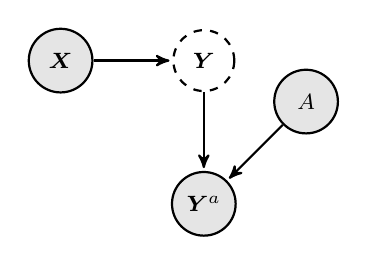
\begin{tikzpicture}[->,>=stealth',shorten >=1pt,auto,node distance=1cm,
  thick,main node/.style={observed},lt/.style={latent}]
 %nodes
\node[lt](1){$\vec{Y}$};
\node[main node, below=of 1](2){$\vec{Y}^a$};
\node[main node, above right=of 2](3){$A$};
\node[main node, left=of 1](4){$\vec{X}$};
 \path[every node/.style={font=\sffamily\small}]
   (4) edge (1)
   (3) edge (2)
   (1) edge (2);
\end{tikzpicture} 
\end{subfigure}
\begin{subfigure}[t]{0.29\textwidth}
\centering
\caption{$\vec{X}$ and $\vec{Y}$ are confounded}
\label{fig:context-graph-confounded}
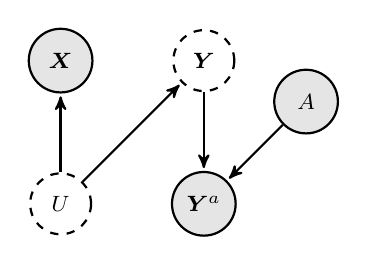
\begin{tikzpicture}[->,>=stealth',shorten >=1pt,auto,node distance=1cm,
  thick,main node/.style={observed},lt/.style={latent}]
 %nodes
\node[lt](1){$\vec{Y}$};
\node[main node, below=of 1](2){$\vec{Y}^a$};
\node[main node, above right=of 2](3){$A$};
\node[main node, left=of 1](4){$\vec{X}$};
\node[lt, below=of 4](5){$U$};
 \path[every node/.style={font=\sffamily\small}]
   (3) edge (2)
   (1) edge (2)
   (5) edge (4) edge (1);
\end{tikzpicture}
\end{subfigure}
\begin{subfigure}[t]{0.29\textwidth}
\centering
\caption{$\vec{Y}$ causes $\vec{X}$}
\label{fig:context-graph-anti-causal}
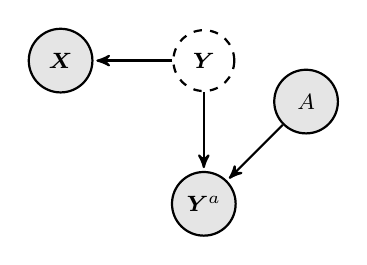
\begin{tikzpicture}[->,>=stealth',shorten >=1pt,auto,node distance=1cm,
  thick,main node/.style={observed},lt/.style={latent}]
 %nodes
\node[lt](1){$\vec{Y}$};
\node[main node, below=of 1](2){$\vec{Y}^a$};
\node[main node, above right=of 2](3){$A$};
\node[main node, left=of 1](4){$\vec{X}$};
 \path[every node/.style={font=\sffamily\small}]
   (1) edge (4)
   (3) edge (2)
   (1) edge (2);
\end{tikzpicture} 
\end{subfigure}
\caption{Several potential causal graphical models for the contextual bandit problem (if actions are selected at random). $\vec{X}$ and $\vec{Y}$ represent the context and reward vectors respectively, and $Y = \vec{Y}^a$ is the reward received by the learner, which is a deterministic function of $\vec{Y}$ and $a$. Regardless of the causal structure, observing the context $\vec{X}$ provides information about the vector of rewards $\vec{Y}$. The causal structures in figures \ref{fig:context-graph-causal} and \ref{fig:context-graph-confounded} also make sense if the elements of $\vec{Y}$ are genuine counterfactuals, that is only the reward of the selected action is ever realised. The context $\vec{X}$ can only be useful in causal graphs of the form in figure \ref{fig:context-graph-anti-causal} if the components of $\vec{Y}$ are realised prior to the agent selecting an action, i.e when the components of $\vec{Y}$ are not truly counterfactual, it just that the agent is limited to only observing the outcome of the action they choose.  To represent a realistic (contextual) bandit problem, where actions are not selected at random, we would need to \quotes{unroll} the graphs, such that there was a copy for each time-step $t$ and allow the action $A_t$ to depend on the context $\vec{X}_t$ and the previous observations $(\vec{X},A,Y)_1^{t-1}$. }
\label{fig:contextual-bandit-causal-graph}
\end{figure}

\vspace{0.5cm}
\begin{example}
\label{exm:anti-casual-context}
Imagine a modified game of roulette. As in standard roulette, it consists of a spinning wheel with a ball that can land in one of 37 numbered pockets. However, unlike the standard game where punters place bets before the wheel is spun, in this variant the wheel is spun first. Five seconds before it comes to rest the face of the wheel darkens to hide the position of the ball from the players. They then place bets after it has stopped (and are each allowed only to check if the position they have bet on was correct). At the point in time the players are selecting their actions, the rewards for each possible choice are fully determined (all zero except for the pocket containing the ball). Suppose a canny gambler realises the ball makes a tiny sound, from rocking back and forth, if it is close to the left or right side of the wheel such that the pocket holding it is close to horizontal. The existence (or not) of this sound is a consequence of the position of the ball and thus the reward state and the gambler can use it as context to improve the likelihood of obtaining a reward.
\end{example}

It is difficult to come up with realistic examples in which the full sequence of rewards is generated, but only the one associated with the selected action is observable to the learner. In the typically cited applications of contextual bandit algorithms, such as selecting how to treat patients or which ad to use, only the reward of the selected action is ever realised, and the alternate rewards are counterfactual variables.

\subsection{Learning from logged bandit data}
\label{sec:off-policy-evaluation}
Another topic of interest within the bandit community, which is deeply connected to causal effect estimation from observational data, is learning from logged bandit feedback data or off-policy evaluation\citep{Langford2008a,strehl2010learning,Li2010,Dudik2011,Bottou2013,Swaminathan2015}. In this setting, the learner has a data set $S = \set{(\vec{X}_t,A_t,\cfb{Y}{A_t})}_{t=1}^T$, which is assumed to have been generated by a stochastic contextual bandit environment interacting with some unknown, potentially stochastic, policy $\pi(\vec{x}_t,h_t)$, where $h_t$ is the sequence of observed data up to time $t$. The goal of the learner is to evaluate the value of an alternate policy, $\pi'$, for selecting actions, often with the underlying motivation of identifying an optimal policy within some space of policies $\Pi$. 

This problem differs from the contextual bandit problem in that the learner is not interacting with the environment. As a result, there is no exploration-exploitation trade-off to be made. However, the problem does not reduce to supervised learning because of the bandit nature of the feedback; only the reward of the selected action is observed. In addition, if $\pi$ is allowed to depend $h$ then the samples are not i.i.d. The majority of the literature considers the case where the original policy $\pi$ was stationary ($\pi(\vec{x}_t,h_t) = \pi(\vec{x})$). \citet{Langford2008a} do allow the original policy to be adaptive and prove a high probability bound on the accuracy of their estimator for $\pi'$, albeit with the strong assumption that the original estimator $\pi$ did not depend on $\vec{X}$. 

If the original policy is assumed to be stationary, the problem of evaluating an alternate policy $\pi'$ is almost identical to that of causal effect estimation under ignorability, as we discussed in section \ref{sec:causal_effect_under_ignorability}. The causal structure can be represented in figure \ref{fig:off-policy-evaluation} There is an (implicit) assumption that all variables that affect the choice of action by $\pi$ are included in $\vec{X}$, ensuring that $\vec{X}$ satisfies the backdoor criterion with respect to identifying the causal effect of $do(A = a)$ on the observed reward $Y$, for any action $a \in \set{1,...,k}$. The only difference is that the goal is to evaluate alternate policies $\pi'$ that may be stochastic and depend on $\vec{x}$, as opposed to only policies of the form $\pi'(x) = a$, equivalent to $do(A=a)$. However, the identification of such stochastic, conditional policies can be reduced to the identification of $\P{y|do(A=a),\vec{x}}$, see section 4.2. of \citet{Pearl2000}. In this case, letting $\Pns{\pi'}{a|\vec{x}}$ denote the distribution over actions under policy $\pi'$ given context $\vec{x}$, the expected (per round) reward obtained by $\pi'$ is given by,

\eqn{
\E{y|\pi'} = \E{y|do(a \sim \pi'(\vec{x}))} = \Esub{(\vec{x},a) \sim \P{\vec{x}}\Pns{\pi'}{a|\vec{x}}}{y|\vec{x},a}
}

As in estimating average causal effects under ignorability, we have a covariate shift problem, with training data sampled from $\P{\vec{x}}\Pns{\pi}{a|\vec{x}}\P{y|\vec{x},a}$ but generalisation error measured with respect to $\P{\vec{x}}\Pns{\pi'}{a|\vec{x}}\P{y|\vec{x},a}$. A difference in practice, is that in the applications frequently considered under learning from logged feedback data, such as ad serving or recommender systems, there may be substantial information available about $\pi$, in the best case, $\Pns{\pi}{a|\vec{x}}$ is known. This makes estimators utilising inverse propensity weighting, including doubly robust estimators as in \citet{Dudik2011}, more attractive. 

\begin{figure}
\centering
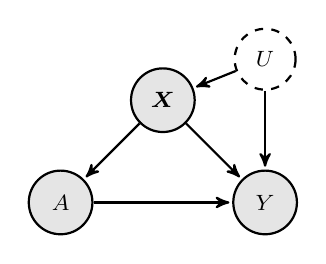
\begin{tikzpicture}[->,>=stealth',shorten >=1pt,auto,node distance=1cm,
  thick,main node/.style={observed},lt/.style={latent}]
\node[main node](1){$\vec{X}$};
\node[main node, below right=of 1](2){$Y$};
\node[main node,  below left=of 1](3){$A$};
\node[lt, above=of 2](4){$U$};
 \path[every node/.style={font=\sffamily\small}]
   (3) edge (2)
   (1) edge (2) edge (3)
   (4) edge (1) edge (2);
\end{tikzpicture} 
\caption{Causal graphical model for learning from logged feedback data under the assumption the original policy $\pi$ for selecting actions was stationary and dependent only on some observed context $\vec{X}$, $a \sim \pi(\vec{x})$. The outcome $Y$ may depend on $\vec{X}$ directly, indirectly through a latent variable $U$ or both.}
\label{fig:off-policy-evaluation}
\end{figure}

\citet{Swaminathan2015} point out that the problem of identifying the optimal policy (subject to some risk minimisation goal) is not as simple as estimating the expected reward associated with each policy in some space and selecting the empirical best because the variance of the estimators for some policies may be much higher than for others.

\subsection{Adding structure to actions}
\label{sec:adding-structure-bandit-actions}

The classic multi-armed bandit is a powerful tool for sequential decision making. However, the regret grows linearly with the number of (sub-optimal) actions and many real world problems have large or even infinite action spaces. This has led to the development of a wide range of models that assume some structure across the reward distributions for different arms, for example generalised linear bandits \citep{filippi2010parametric}, dependent bandits \citep{Pandey2007}, X-armed bandits \citep{Bubeck2010} and Gaussian process bandits \citep{srinivas2009gaussian}, or that consider more complex feedback, for example the recent work on graph feedback\citep{Mannor2011,Lelarge2012,Alon2013,Buccapatnam2014,Kocak2014,Alon2015} and partial monitoring \citep{Piccolboni2001,Bartok2014}.

In the next chapter, I propose a very natural connection between causal graphs and bandit problems and show it induces a novel form of additional feedback and structure between arms that cannot be can exploited by any of these previous approaches. 

\section{The counterfactual nature of regret}
\label{sec:counterfactual-nature-regret}

We conclude this chapter on bandits with a note on the counterfactual nature of regret, which has not been discussed with respect to bandit regret. However, the issues raised are very closely related to the work by \citet{Dawid2000} on problems associated with the use of counterfactual variables for (observational) causal inference.

It is possible, as we demonstrated in example \ref{exm:anti-casual-context}, to construct bandit problems in which the full vector of rewards $[\cfb{Y}{1},...,\cfb{Y}{k}]$ is actually generated at each time-step (and, at least in principle, is observable to someone although not the agent). However, in most real applications for bandit problems, only the outcome associated with the selected action is ever realised and so the remaining components of the reward vector are counterfactual, justifying the use of the counterfactual notation to denote them. There are complex philosophical objections to counterfactuals arising from the way they describe alternate universes that were never realised. This makes it easy to make statements using counterfactuals that cannot be confirmed empirically (even with infinite experimental data). We now show with a simple example that the standard definition of regret is a fundamentally counterfactual quantity. Recall that the cumulative regret is defined by,

\eqn{
\label{eqn:raw_regret2}
\rawregret &= \sum_{t=1}^T \cfb{Y}{i^*} - \sum_{t=1}^T \cfb{Y}{a_t}
\\&= \sum_{t=1}^T \left(\cfb{Y}{i^*} - \cfb{Y}{a_t}\right)
}

Take a stochastic, two-armed, Gaussian bandit with the joint distribution of the (counterfactual) rewards $\P{\cfb{Y}{1},\cfb{Y}{2}}$ given by equation \ref{eqn:joint-gaussain-reward}. Suppose without loss of generality that arm 1 is the optimal arm, such that $\mu_1 > \mu_2$.  

% vector with mean mu_t,mu_c and a covariance matrix
\eqn{
\label{eqn:joint-gaussain-reward}
P(\cfb{Y}{1},\cfb{Y}{2}) \sim N( 
         \begin{bmatrix}
           \mu_{1} \\
           \mu_2 \\
         \end{bmatrix},
         \begin{bmatrix}
           \sigma^2 & \rho \sigma^2 \\
           \rho \sigma^2 & \sigma^2 \\
         \end{bmatrix}
         )
}

Consider an algorithm that always selects arm 2.  The distribution over the difference of jointly normal random variables is also normal, letting, $\tau_t = \cfb{Y}{1} - \cfb{Y}{2}$ yields $\P{\tau_t} = N(\mu_1 - \mu_2,2\sigma^{2}(1-\rho))$. Thus the distribution over the regret for this algorithm is given by,

\eqn{
\rawregret \sim N\left(T(\mu_1 - \mu_2), 2\sigma^2 T(1-\rho)\right)
}

The parameters of the marginal distributions, $\P{\cfb{Y}{1}}$ and $\P{\cfb{Y}{2}}$, can be estimated directly by simply sampling from each arm. However, the covariance $\rho$ cannot, because we never simultaneously observe the rewards for both arms. As a result, even with full knowledge of the reward distributions for each arm, the distribution over regret cannot, in general, be computed without un-testable assumptions about the covariance between counterfactuals (see figure \ref{fig:metaphysical_distribution_difference}). 

\begin{figure}[h]
\captionsetup[subfigure]{position=b}
\centering
\subcaptionbox{Marginal distributions over the rewards for each action for $\mu_1=1$, $\mu_2=0$ and $\sigma = 1$. \label{fig:metaphys_a}}{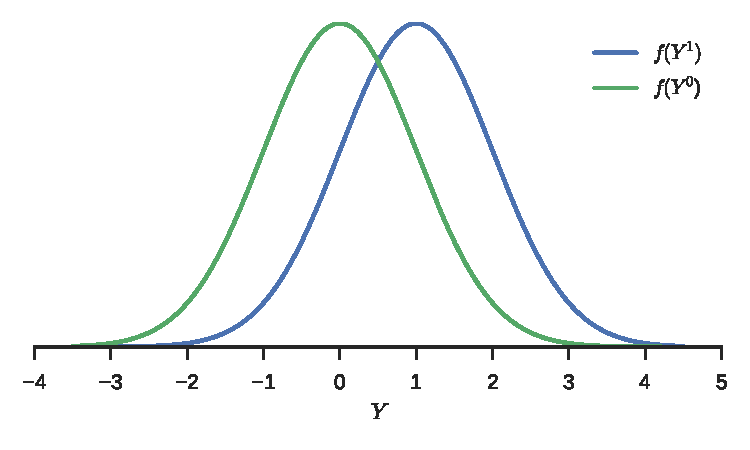
\includegraphics[width=.45\linewidth]{figures/counterfactual_nonidentify_a.pdf}}
\hspace{0.02\textwidth}
\subcaptionbox{The distribution over $R_T$ for $T=10$ for two different values of $\rho$ \label{fig:metaphys_b}}
{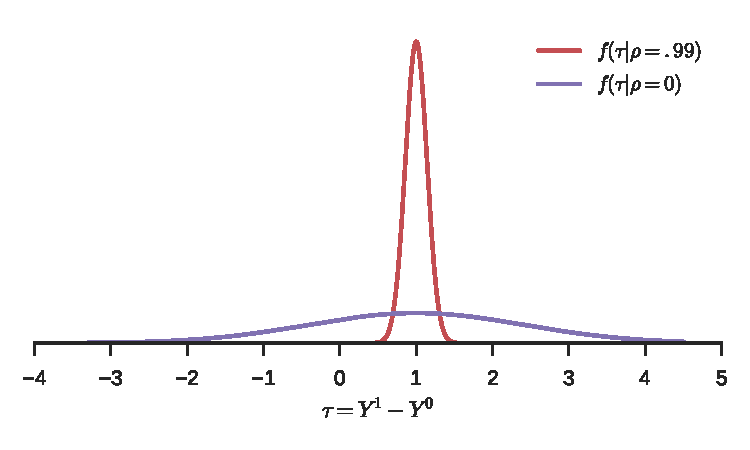
\includegraphics[width=.45\linewidth]{figures/counterfactual_nonidentify_b.pdf}}
\caption{The distribution over the regret as defined by equation \ref{eqn:raw_regret2} depends on unobservable properties of the joint distribution over counterfactual rewards. The same (marginal) distributions over the rewards can correspond to quite different regret distributions.}
\label{fig:metaphysical_distribution_difference}
\end{figure}

This result is somewhat perturbing. The stochastic bandit problem can be defined without recourse to counterfactual variables by having the world stochastically generate only a reward for the selected action at each timestep, and the behaviour of standard bandit algorithms depends only on the marginal reward distributions for each arm. The expectation of the regret as defined by equation \ref{eqn:pseudo_regret} also remains unchanged as both its definition and the learner's actions depend only on the marginal distributions. It seems therefor unfortunate that we should have to assume, for example, that the rewards for alternate actions are independent of one-another to be able to analyse the variance of the regret. This is particularly so, as this assumption is likely to be violated in many realistic bandit problems. For example, a given user may be more (or less) likely to buy something no matter which advertisement they are served, leading to a positive correlation between counterfactual rewards. Equally, an illness might have two (unobservable) sub-types, with each medication (bandit arm) effective only against one, resulting in a negative correlation between the counterfactual rewards. 

We could focus only on analysing the expected regret, since this depends only on the marginal distributions. However, there are many real problems for which we do care how tightly concentrated the regret is around its expectation. For example, if we are risk averse, we may prefer an algorithm with slightly higher expected regret but a lower probability of suffering extremely large regret. This raises the question, is it possible to construct an alternate definition of regret that can capture how consistently bandit algorithms behave, but that does not depend on any properties of the joint distribution over counterfactual rewards? A natural candidate would be:

\eqn{
R_T = \sum_{i=1}^k N_i(T)\Delta_i, 
}

where $N_i(T)$ is the number of times arm $i$ was played up to timestep $T$ and $\Delta_i$ is the degree to which arm $i$ is sub-optimal, $\Delta_i = \mu^* - \mu_i$. The expectation of this variant of regret is the same as for the standard version defined in equation \ref{eqn:raw_regret2}. It depends only on the randomness of the reward distribution only indirectly through the number of times each action is selected, which in turn depends only on the marginal distributions. Furthermore, this quantity has already been analysed in existing work on the concentration of bandit regret, \citep{Audibert2007,Audibert2009exploration} as a more tractable proxy to the standard regret. In conclusion, when selecting measures of bandit performance, it is worth noting whether they rely on counterfactual assumptions and considering if these assumptions are justifiable or needed for the specific problem on interest.


\chapter{Causal Bandits: Unifying the approaches}
\label{chap:causal-bandit}

As we have seen in the previous two chapters, critical insights and methods for learning how to act have emerged from both the observational and experimental approaches to causality. From observational inference, we have the do-calculus, which allows us to map information between observational and interventional distributions and we have a range of estimators designed for these types of mapping problems including propensity scores and doubly robust methods. The bandit community has developed carefully tuned algorithms to balance exploration and exploitation, estimation approaches for identifying and selecting the optimal action (rather than estimating the rewards for all actions) and techniques to bound the bias of estimators due to the adaptive nature of decision making processes.

However, despite the commonality of the underlying problem, there has been relatively little work on the intersection between observational causal inference and adaptive decision making processes. Although some ideas, such as doubly robust estimators and inverse propensity score weighting have transferred across (from causal inference to off-policy evaluation), there are many more opportunities for fruitful work in this space. In most key real world decision making processes, from algorithms recommending drug treatments to robots deciding how to open doors, we have access to both potentially huge observational data sets, as well as the ability to intervene in the system at some level. It is critical that we develop methods that allow us to incorporate the causal knowledge we have about the world, along with data sets collected under a range of different conditions, into our current decision making process. In this chapter, I introduce a very general framework that connects causal graphical models with multi-armed bandit problems and demonstrate how it can be leveraged to make better decisions.


\section{A framework to connect bandit problems with observational causal inference}
\label{sec:intro_causal_bandit}
A natural way to connect the causal framework with the bandit setting is to model the action space as interventions on variables in a causal directed acyclic graph. Each possible assignment of variables to values is a potential action (or bandit arm), see figure \ref{fig:unify_frameworks} for a simple example. In some settings, it makes sense to restrict the action space available to the agent to a subset of all the possible actions, for example the set of single variable interventions. The reward could be a general function of the action selected and the final state of the graph. However, for simplicity, we will consider the reward to be the value of a single specified node. We refer to these problems as \emph{causal bandit problems}. In this thesis, I focus on the case where the causal graph is known. Extending this work to simultaneously learning the casual graph is discussed in \S\ref{sec:causal_bandit_discussion}.

\begin{figure}
\centering
\begin{subfigure}[c]{0.3\textwidth}
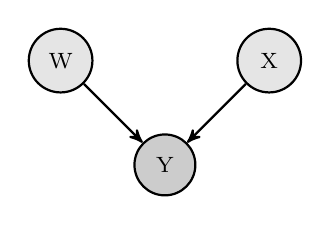
\begin{tikzpicture}[->,shorten >=0pt,shorten <=0pt,node distance=3em,thick,main node/.style={observed}, tg/.style={target}]
\node[main node](1){W};
\node[tg, below right=of 1](2){Y};
\node[main node, above right=of 2](3){X};
\path[]
	(1) edge (2)
	(3) edge (2);
\end{tikzpicture}
\end{subfigure}
\begin{subfigure}[t]{0.4\textwidth}
$\actionspace$ = \begin{tabular}{|c|}
	\hline
  $do(W=0,Z=0)$ \\
  $do(W=0,Z=1)$ \\
  $do(W=1,Z=0)$ \\
  $do(W=1,Z=1)$ \\
  \hline
  $do(W=0)$ \\
  $do(W=1)$ \\
  $do(Z=0)$ \\
  $do(Z=1)$ \\
  $do()$ \\
  \hline
\end{tabular}
\end{subfigure}
\caption{A simple causal graphical model and corresponding complete action space. $W$ and $Z$ represent binary variables that can be intervened on and $Y$ represents the reward.}
\label{fig:unify_frameworks}
\end{figure} 

The type of problem we are concerned with is best illustrated with an example. Consider a farmer wishing to optimise the yield of her crop. She knows that crop yield is only affected by temperature, a particular soil nutrient, and moisture level but the precise effect of their combination is unknown. In each season the farmer has enough time and money to intervene and control at most one of these
variables: deploying shade or heat lamps will set the temperature to be low or high; the nutrient can be added or removed through a choice of fertiliser; and irrigation or rain-proof covers will keep the soil wet or dry. Where there is no intervenion, the temperature, soil, and moisture vary naturally from season to season due to weather conditions. These are all observed along with the final crop yield at the end of each season. How might the farmer best experiment to identify the single, highest yielding intervention in a limited number of seasons?

We now formalise the definition of causal bandit problems. We will assume each variable only takes on a finite number of distinct values. (The path to relaxing this assumption would be through levering the work on continuous armed bandits). 

\vspace*{.5cm}
\begin{definition}[Causal bandit problem]
A learner for a casual bandit problem is given the casual model’s graph $G$ over variables $\mathcal{X}$ and a set of allowed actions $\actionspace$. Each action $a \in \actionspace$, denoted $do(\vec{X}=\vec{x})$, assigns values $\vec{x}$ to a corresponding set of variables $\vec{X} \subset \mathcal{X}$ and incurs a known cost $C(a)$ on the learner. One variable $Y \in \mathcal{X}$ is designated as the \emph{reward variable}.

The causal bandit game proceeds over $T$ rounds. In each round $t$, the learner:
\begin{enumerate}
\item \emph{observes} the value of a subset of the variables $\vec{X}^c_t$,
\item \emph{intervenes} by choosing $a_t = do(\vec{X}_t = \vec{x}_t) \in \mathcal{A}$ based on previous observations and rewards, 
\item \emph{observes} values for another subset of variables $\vec{X}^o_t$ drawn from $\P{\vec{X}^o_t |\vec{X}^c_t, do(\vec{X}_t = \vec{x}_t)}$,
\item \emph{obtains reward} $r_t = Y_t - C(a_t)$, where $Y_t$ is sampled from $\P{Y_t| \vec{X}^c_t, do(\vec{X}_t = \vec{x}_t)}$
\end{enumerate} 
\end{definition}

We refer to the set of variables that can be observed prior to selecting an action $\vec{X}^c$ as contextual variables and the set of variables observed after the action is chosen, $\vec{X}^o$, as post-action feedback variables. Note that $\vec{X}^c$ and $\vec{X}^o$ need not be disjoint. A variable may be observed both prior to and after the agent selects an action, and the action may change its value. The notation $\P{\cdot|\vec{X}^c_t, do(\vec{X}_t = \vec{x}_t)}$ denotes distributions conditional on having observed $\vec{X}^c_t$ and \emph{then} intervened to set $\vec{X}_t = \vec{x}_t$. The values of variables in $\vec{X}^c_t$ that are non-descendents of $\vec{X}_t$ remain unchanged by the intervention. The objective of the learner is to minimise either the simple (equation \ref{eqn:simple_regret}) or cumulative regret (equation \ref{eqn:pseudo_regret}). 

The empty intervention (where no variable is set) is denoted $do()$. The \emph{parents} of a variable $X_i$, denoted $\parents{X_i}$, is the set of all variables $X_j$ such that there is an edge from $X_j$ to $X_i$ in $\mathcal{G}$. We denote the expected reward for the action $a = do(\vec{X} = \vec{x})$ by $\mu_{a} := \E{Y | do(\vec{X} = \vec{x})}$ and the optimal expected reward by $\mu^* := \max_{a\in\actions} \mu_{a}$. 

The causal bandit problem takes on characteristics of different bandit settings depending on the action-space $\actionspace$ and corresponding costs, which variables are observable prior to selecting an action, and on which variables we receive post-action feedback. If we can (cheaply) intervene on all of the parents of $Y$ simultaneously then any context or alternative actions are irrelevant, and the problem reduces to a standard multi-armed bandit problem. 

%This is formalised in theorem \ref{theorem:cb-intervene-all-parents}. 

If feedback is received only on the reward node $\vec{X}^o = \set{Y}$, as in the standard bandit setting, then the do-calculus can be applied to eliminate some actions immediately, before any experiments are performed and then a standard bandit algorithm can be run on the remaining actions, see figure \ref{fig:cholesterol_graph} as an example. If we receive post-action feedback on additional nodes the problem can be more interesting. In addition to being able to eliminate some actions prior to sampling any data as in the previous case, taking one action may give us some information on actions that were not selected. Consider again the model in figure \ref{fig:unify_frameworks}. The causal structure implies: 

\eq{
P(Y|do(W = 0)) &= P(Y|do(),W = 0) \\
&= P(Y|do(X=0),W=0)P(X=0)+P(Y|do(X=1),W=0)P(X=1) 
}

\begin{figure}
\centering
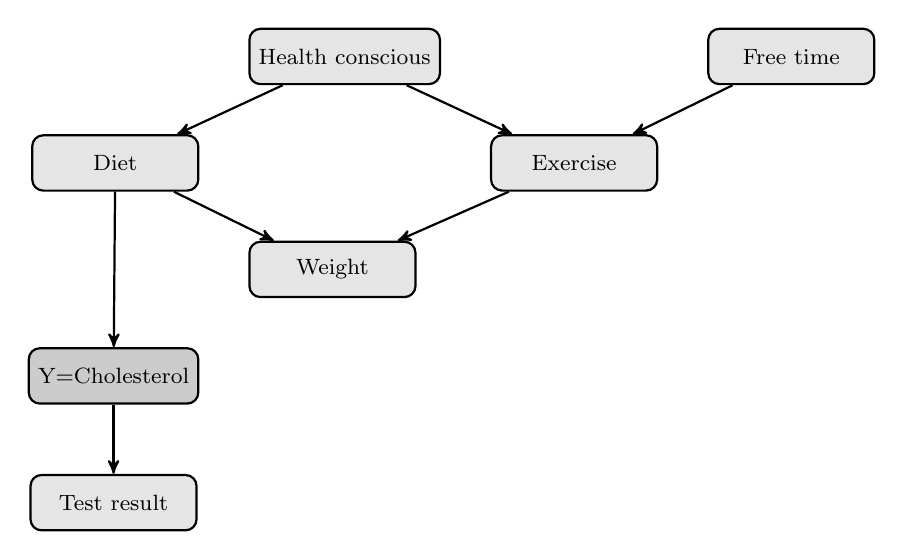
\begin{tikzpicture}[->,shorten >=0pt,shorten <=0pt,node distance=2.5em,thick,node/.style={observedrect},tg/.style={targetrect}]
\node[node](1){Health conscious};
\node[node, below left=of 1](2){Diet};
\node[node, below right=of 1](3){Exercise};
\node[node, below right=of 2](4){Weight};
\node[tg,below left=of 4](5){Y=Cholesterol};
\node[node, below =of 5](6){Test result};
\node[node, above right=of 3](7){Free time};
\path[]
	(1) edge (2) edge (3)
	(2) edge (4) edge (5)
	(3) edge (4)
	(5) edge (6)
	(7) edge (3);
\end{tikzpicture}
\caption{Example causal graph (based on \citet{Koller2009}) where the outcome of interest (reward) is cholesterol level . The do-calculus can be applied to eliminate some actions immediately without the need to do any experiments. For example, no actions involving 'Test Result' need to be considered and interventions on 'Diet' do not need to be considered in conjunction with any other variables.}
\label{fig:cholesterol_graph}
\end{figure}

Thus we gain information about the reward for the action $do(W=0)$ from selecting the action $do()$ or $do(X = x)$ and then observing $W = 0$.  We only get this form of side information for actions that do not specify the value of every variable, for example those in the bottom half of the table in figure \ref{fig:unify_frameworks}. If additional variables are only observed before an intervention is selected, the causal bandit problem can be treated as a stochastic contextual bandit problem, which is already reasonably well understood \citep{Agarwal2014}.

Two other problems that sit in the space between causal inference and bandit problems - bandits with unobserved confounders \cite{Bareinboim2015} and compliance aware bandits  \citep{DellaPenna2016} - can also be viewed as specific causal bandit problems. In the work on bandits with unobserved confounders, it is assumed that the reward given each action may depend on some latent variable $U$, which we cannot observe directly. However, prior to selecting an action, we can observe  $I$, the action that would have been selected under an alternate (stationary) policy, which may depend on $U$, see figure \ref{fig:confounded-causal-bandit-graph}. In this case, the set of contextual variables $\vec{X}^c = I$, the set of post-action feedback variables $\vec{X}^o = \set{Y}$ and the action space consists of all possible assignments of values to a single node $X$, $\actionspace = do(X=x)$. This setting reduces to a contextual bandit problem in our causal bandit framework. However in their work on bandits with unobserved confounders, \citet{Forney2017} also leverage the fact that $I$ represents the action that would have been selected under an alternate policy to fuse data collected under the previous (observational) policy with data collected under the new policy. This information is not encoded in the causal bandit graph in figure \ref{fig:confounded-causal-bandit-graph}, as $I$ could be any variable that is influenced by the unobserved context $U$, and thus cannot be exploited by a standard contextual bandit algorithm. 

Compliance-aware bandits describe situations in which the action recommended by the bandit algorithm is not always followed. For example, a patient may refuse to take a treatment or an advertiser may have complex rules about how many advertisements a given customer can receive, which prevents some of the suggestions from the ad recommendation engine from being followed. After an action is selected, the algorithm can observe the action that was actually taken, in addition to the reward. \citet{DellaPenna2016} analyse this setting with binary treatments both with and without the presence of a latent confounding variable $U$, see figure \ref{fig:imperfect-compliance-causal-bandit-graph}. In this case, there are no contextual variables and the action space is again the set of assignments to a single variable but there is post-action feedback, which reveals the value of the action that was actually taken.\footnote{There are some interesting variants of the compliance aware bandit setting that, to my knowledge, have not been analysed. The first is if the confounding variable $U$ is observable, either as context or post-action feedback. The second is if we extend the allowable action set to include acting directly on $X$, albeit at a higher cost than acting on $A$. It is also worth noting the connection between this setting and instrumental variables \cite{balke1997bounds}. By making some functional assumptions about the relationships between the variables, we can use $A$ as an instrumental variable to bound or estimate the (casual) effect of $X$ on $Y$. The estimation will be complicated in the bandit setting because the action chosen at each timestep is dependent on the previous sequence of actions and rewards.}

\begin{figure}[h]
\centering
\begin{subfigure}[t]{0.49\textwidth}
\centering
\caption{Bandits with unobserved confounders:$\vec{X}^c=\set{I}$, $\vec{X}^o = \set{Y}$, $\actionspace = do(X=x)$}
\label{fig:confounded-causal-bandit-graph}
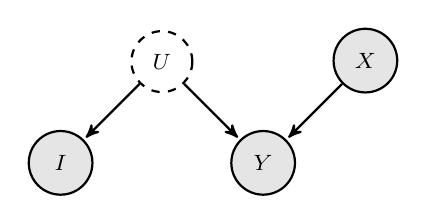
\begin{tikzpicture}[->,>=stealth',shorten >=1pt,auto,node distance=1cm,
  thick,main node/.style={observed},lt/.style={latent}]
 %nodes
\node[lt](1){${U}$};
\node[main node, below right =of 1](2){${Y}$};
\node[main node, below left=of 1](3){$I$};
\node[main node, above right=of 2](4){$X$};
 \path[every node/.style={font=\sffamily\small}]
   (1) edge (2) edge (3)
   (4) edge (2);
\end{tikzpicture} 
\end{subfigure}
\begin{subfigure}[t]{0.49\textwidth}
\centering
\caption{Compliance aware bandits: $\vec{X}^c=\set{}$, $\vec{X}^o = \set{T,Y}$, $\actionspace = do(X=x)$ }
\label{fig:imperfect-compliance-causal-bandit-graph}
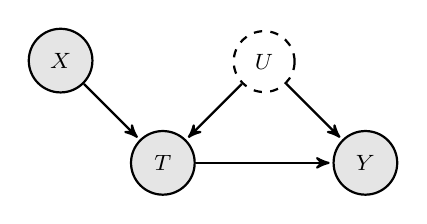
\begin{tikzpicture}[->,>=stealth',shorten >=1pt,auto,node distance=1cm,
  thick,main node/.style={observed},lt/.style={latent}]
 %nodes
\node[lt](1){$U$};
\node[main node, below left=of 1](2){$T$};
\node[main node, below right=of 1](3){$Y$};
\node[main node, above left=of 2](4){$X$};
 \path[every node/.style={font=\sffamily\small}]
   (1) edge (2) edge (3)
   (2) edge (3)
   (4) edge (2);
\end{tikzpicture} 
\end{subfigure}
\caption{}
\label{fig:causal-bandit-version-confounded-compliance}
\end{figure}

The classical $K$-armed stochastic bandit problem can be recovered in our framework by considering a simple causal model with one edge connecting a single variable $X$ that can take on $K$ values to a reward variable $Y \in \set{0,1}$ where $\P{Y = 1|X} = r(X)$ for some arbitrary but unknown, real-valued function $r$. The set of allowed actions in this case is $\mathcal{A} = \{ do(X = k) \colon k \in \{1, \ldots, K\}\}$. Conversely, any causal bandit problem can be reduced to a classical stochastic $|\mathcal{A}|$-armed bandit problem by treating each possible intervention as an independent arm and ignoring all sampled values for the observed variables except for the reward. However, the number of actions or arms grows exponentially with the number of variables in the graph making it important to develop algorithms that leverage the graph structure and additional observations.

\section{Causal bandits with post action feedback}
\label{sec:causal-bandit-post-action-feedback}

We now focus on causal bandit problems with post-action feedback, in which the value of all the variables are observed after an intervention is selected, the cost of all allowable actions is equal and the goal of the learner is to minimise the simple regret. I presented this work at NIPS 2016 \citep{NIPS2016_6195}.

\paragraph{Related Work} As alluded to above, causal bandit problems can be treated as classical multi-armed bandit problems by simply ignoring the causal model and extra observations and applying an existing best-arm identification algorithm with well understood simple regret guarantees \citep{Jamieson2013}. However, as we show in \S\ref{sec:simple-regret}, ignoring the extra information available in the non-intervened variables yields sub-optimal performance.

Our framework bears a superficial similarity to contextual bandit problems, \S\ref{sec:contextual-bandits}, since the extra observations on non-intervened variables might be viewed as context for selecting an intervention. 
However, a crucial difference is that in our model the extra observations are only revealed \emph{after} selecting an intervention and hence cannot be used as context. 

There have been several proposals for bandit problems where extra feedback is received after an action is taken.
Most recently, \citet{Alon2015}, \citet{Kocak2014} have considered very general models related to partial monitoring games~\citep{Bartok2014} where rewards on un-played actions are revealed according to a feedback graph. As we discuss in \S\ref{sec:causal_bandit_discussion}, the parallel bandit problem can be captured in this framework. However, the regret bounds are not optimal in our setting. They also focus on cumulative regret, which cannot be used to guarantee low simple regret~\citep{Bubeck2009a}. The partial monitoring approach taken by \citet{wu2015online} could be applied (up to modifications for the simple regret) to the parallel bandit, but the resulting strategy require knowledge about the likelihood of each factor in advance, while our strategy learns this online. \citet{Yu2009} utilise extra observations to detect changes in the reward distribution, whereas we assume fixed reward distributions and use extra observations to improve arm selection. \citet{Avner2012} analyse bandit problems where the choice of arm to pull and arm to receive feedback on are decoupled. The main difference from our present work is our focus on simple regret and the more complex information linking rewards for different arms via causal graphs. To the best of our knowledge, our paper is the first to analyse simple regret in bandit problems with extra post-action feedback.


%\citet{Yu2009} consider bandit problems where a learner chooses an arm to play as well as set of arms to observe rewards for in a stochastic setting where the reward distributions can change infrequently and the aim is to minimize cumulative regret. They use extra observations to detect changes whereas we assume fixed reward distributions and use extra observations to improve arm selection.
% Partial monitoring is a very general framework for for decoupling the feedback from the action and reward. It can be used to classify problems into one of four categories, trivial with no regret, easy with $R_T = \bigthetatilde{\sqrt{T}}$ , hard with $R_T = \bigtheta{T^{2/3}}$ and hopeless with $R_T = \bigomega{T}$ \citep{Bartok2014}. Partial monitoring algorithms yield results that are optimal with respect the horizon $T$ but not other parameters, such as $K$, which is the key focus of incorporating causal structure. 

Two pieces of recent work also consider applying ideas from causal inference to bandit problems.\citet{Bareinboim2015} demonstrate that in the presence of confounding variables the value that a variable would have taken had it not been 
intervened on can provide important contextual information. Their work differs from this thesis in many ways. For example, the focus is on the cumulative regret, and the context is observed before the action is taken and cannot be controlled by the learning agent.  

%\todof{write one sentence to explain how their work is different to ours}

\citet{Ortega2014thompson} present an analysis and extension of Thompson sampling, assuming actions are causal interventions. Their focus is on causal induction (\ie, learning an unknown causal model) instead of exploiting a known causal model. Combining their handling of  causal induction with our analysis is left as future work.
% Key to Elias' paper is: observing the action an agent would take if it were allowed to make its natural choice can provide some information about hidden confounders that influence both the reward and the choice of action. Therefore, incorporating an agents natural choice as context may outperform a standard bandit that does not use that context. (Note: even in the presence of hidden confounders, including the agents natural choice as context only may improve the results. It is easy to come up with a counter example in which it does not).

The truncated importance weighted estimators used in \S\ref{sec:simple-regret-general} have been studied before in a causal framework by \citet{Bottou2013}, 
where the focus is on learning from observational data, but not controlling the sampling process. They also briefly discuss some of the issues 
encountered in sequential design, but do not give an algorithm or theoretical results for this case.


\subsection{The parallel bandit problem}
\label{sec:simple-regret}
In this section, we propose and analyse an algorithm for achieving the optimal regret in a natural special case of the causal bandit problem, which we call the {\it parallel bandit}.
It is simple enough to admit a thorough analysis but rich enough to model the type of problem discussed in \S\ref{sec:intro_causal_bandit}, including the farming example. It also suffices to witness the regret gap between algorithms that make use of causal models and those that do not.

The causal model for this class of problems has $N$ binary variables $\{ X_1, \ldots, X_N \}$ where each $X_i \in \{0,1\}$ are independent causes of a reward variable $Y \in \set{0,1}$, as shown in Figure~\ref{fig:parallel}. All variables are observable and the set of allowable actions are all size 0 and size 1 interventions: $\mathcal{A} = \set{do()} \cup \set{ do(X_i = j) \colon 1 \leq i \leq N \text{ and } j \in \set{0,1}}$

In the farming example above, $X_1$ might represent temperature (\eg, $X_1=0$ for low and $X_1=1$ for high). The interventions $do(X_1 = 0)$ and $do(X_1 = 1)$ indicate the use of shades or heat lamps to keep the temperature low or high, respectively.

\begin{figure}
    \begin{subfigure}[t]{0.34\textwidth}
	\centering   
	 \caption{Parallel graph}\label{fig:parallel} 
          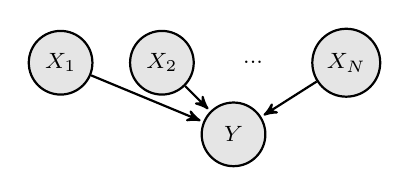
\begin{tikzpicture}[->,>=stealth',shorten >=1pt,auto,node distance=.45cm,
  thick,main node/.style={observed}, hidden/.style={empty},background rectangle/.style={fill=olive!45}]
%every node/.style={scale=0.6}
 %nodes
\node[main node](1){$X_{1}$};
\node[main node, right=of 1](2){$X_{2}$};
\node[hidden, right=of 2](3){$...$};
\node[main node, right=of 3](4){$X_{N}$};
\node[main node, below right=of 2](5){$Y$};
 \path[every node/.style={font=\tiny}]
    (1) edge (5)
    	(2) edge (5)
    (4) edge (5);
\end{tikzpicture} 
\end{subfigure}
    \begin{subfigure}[t]{0.25\textwidth}
    \centering
     \caption{Confounded graph}
        \label{fig:causalStructure_confounded}
        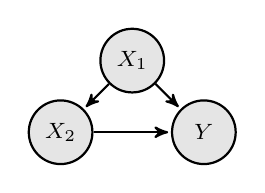
\begin{tikzpicture}[->,>=stealth',shorten >=1pt,auto,node distance=.45cm,
  thick,main node/.style={observed}, hidden/.style={empty},background rectangle/.style={fill=olive!45}]
\node[main node](1){$X_1$};
\node[main node, below left=of 1](2){$X_2$};
\node[main node, below right=of 1](4){$Y$};
 \path[every node/.style={font=\tiny}]
    (1) edge (2)
    (1) edge (4)
    (2) edge (4);
\end{tikzpicture}
    \end{subfigure}
    \begin{subfigure}[t]{0.4\textwidth}
    \centering
     \caption{Chain graph}
        \label{fig:causalchain}
         \begin{tikzpicture}[->,>=stealth',shorten >=1pt,auto,node distance=.45cm,
  thick,main node/.style={observed}, hidden/.style={empty},background rectangle/.style={fill=olive!45}]
\node[main node](1){$X_{1}$};
\node[main node, right=of 1](2){$X_{2}$};
\node[hidden, right=of 2](3){$...$};
\node[main node, right=of 3](4){$X_{N}$};
\node[main node, right=of 4](5){$Y$};
 \path[every node/.style={font=\tiny}]
    (1) edge (2)
  	(2) edge (3)
    (3) edge (4)
    (4) edge (5);
\end{tikzpicture}
    \end{subfigure}
      \caption{Causal Models}\label{fig:causalmodels}\label{fig:causal_models_causal_bandit}
\end{figure}


In each round the learner either purely observes by selecting $do()$ or sets the value of a single variable. The remaining variables are simultaneously set by independently biased coin flips. The value of all variables are then used to determine the distribution of rewards for that round. Formally, when not intervened upon we assume that each $X_i \sim \bernoulli(q_i)$ where $\vec{q} = (q_1, \ldots, q_N) \in [0,1]^N$ so that $q_i = \P{X_i = 1}$.

The value of the reward variable is distributed as $\P{Y = 1|\vec{X}} = r(\vec{X})$ where 
$r : \{0,1\}^N \to [0,1]$ is an arbitrary, fixed, and unknown function. 
In the farming example, this choice of $Y$ models the success or failure of a seasons crop, 
which depends stochastically on the various environment variables.


\paragraph{The Parallel Bandit Algorithm}
%\label{sub:par-bandit-alg}
The algorithm operates as follows. For the first $T/2$ rounds it chooses $do()$ to collect observational data. As the only link from each $X_1,\ldots,X_N$ to $Y$ is a direct, causal one, $\P{Y|do(X_i=j)}=\P{Y|X_i=j}$. Thus we can create good estimators for the returns of the actions $do(X_i = j)$ for which $\P{X_i = j}$ is large. The actions for which $\P{X_i = j}$ is small may not be observed (often) so  estimates of their returns could be poor. To address this, the remaining $T/2$ rounds are evenly split to estimate the rewards for these infrequently observed actions. The difficulty of the problem depends on $\vec{q}$ and, in particular, how many of the variables are unbalanced (\ie, small $q_i$ or $(1-q_i)$). For $\tau \in [2...N]$ let $I_\tau = \set{ i : \min\set{q_i, 1-q_i} < \frac{1}{\tau}}$. Define

\eq{
\label{eq:m-simple}
m(\vec{q}) = \min \set{ \tau : |I_{\tau}| \leq \tau}\,.
}


\begin{algorithm}[H]
\caption{Parallel Bandit Algorithm}\label{alg:simple}
\begin{algorithmic}[1]
\STATE {\bf Input:} Total rounds $T$ and $N$.
\FOR{$t \in 1,\ldots,T / 2$}
\STATE Perform empty intervention $do()$
\STATE Observe $\vec{X}_t$ and $Y_t$
\ENDFOR
\FOR{$a = do(X_i = x) \in \actions$}
\STATE Count times $X_i = x$ seen: $T_a = \sum_{t=1}^{T/2} \ind{X_{t,i} = x}$
\STATE Estimate reward: $\hat{\mu}_a = \frac{1}{T_a} \sum_{t=1}^{T/2} \ind{X_{t,i} = x} Y_t$ \\[0.2cm]
\STATE Estimate probabilities: $\hat{p}_a = \frac{2 T_a}{T}$,\,\, $\hat q_i = \hat p_{do(X_i = 1)}$
\ENDFOR
\STATE Compute $\hat{m} = m(\vec{\hat q})$ and $A = \set{a \in \actions \colon \hat{p}_a \leq \frac{1}{\hat m}}$.
\STATE Let $T_A := \frac{T}{2 |A|}$ be times to sample each $a\in A$.
\FOR{$a = do(X_i = x) \in A$}
\FOR{$t \in 1,\ldots,T_A$}
\STATE Intervene with $a$ and observe $Y_t$
\ENDFOR
\STATE Re-estimate $\hat{\mu}_a = \frac{1}{T_A} \sum_{t=1}^{T_A} Y_t$
\ENDFOR
\RETURN estimated optimal $\hat{a}^*_T \in \argmax_{a\in\actions} \hat{\mu}_a$
\end{algorithmic}
\end{algorithm}

$I_\tau$ is the set of variables considered unbalanced and we tune $\tau$ to trade off identifying the low probability actions against not having too many of them, so as to minimise the worst-case simple regret. When $\vec{q} = (\frac{1}{2}, \ldots, \frac{1}{2})$ we have $m(\vec{q}) = 2$ and when $\vec{q} = (0, \ldots, 0)$ we have $m(\vec{q}) = N$. We do not assume that $\vec{q}$ is known, thus Algorithm \ref{alg:simple} also utilises the samples captured during the observational phase to estimate $m(\vec{q})$. Although very simple, the following two theorems show that this algorithm is effectively optimal.


\begin{theorem}\label{thm:uq-simple}
Algorithm \ref{alg:simple} satisfies
\eq{
\simpleregret \in \bigo{\sqrt{\frac{m(\vec{q})}{T}\log\left(\frac{NT}{m(\vec{q})}\right)}}\,.
}
\end{theorem}


\begin{theorem}\label{thm:lower}
For all strategies and $T$, $\vec{q}$, there exist rewards such that
$\displaystyle \simpleregret 
\in \Omega\left(\sqrt{\frac{m(\vec{q})}{T}}\right)$.
\end{theorem}

The proofs of Theorems \ref{thm:uq-simple} and \ref{thm:lower} follow by carefully analysing the concentration
of $\hat p_a$ and $\hat m$ about their true values and may be found in Sections \ref{sec:thm:uq-simple} and \ref{sec:thm:lower} respectively.

%We prove a lower bound on the simple regret that matches up to logarithmic factors the upper bound given in Theorem \ref{thm:uq-simple}. 
By utilising knowledge of the causal structure, Algorithm \ref{alg:simple} effectively only has to explore the $m(\vec{q})$ 'difficult' actions. Standard multi-armed bandit algorithms must explore all $2N$ actions and thus achieve regret  $\smash{\Omega(\sqrt{N/T})}$. Since $m$ is typically much smaller than $N$, the new algorithm can significantly outperform classical bandit algorithms in this setting. In practice, you would combine the data from both phases to estimate rewards for the low probability actions. We do not do so here as it slightly complicates the proofs and does not improve the worst case regret.

\subsection{General graphs}
\label{sec:simple-regret-general}
We now consider the more general problem where the graph structure is known, but arbitrary. For general graphs, $\P{Y|X_i=j} \neq \P{Y|do(X_i=j)}$ (correlation is not causation). However, if all the variables are observable, any causal distribution $\P{X_1...X_N|do(X_i=j)}$ can be expressed in terms of observational distributions via the truncated factorisation formula \citep{Pearl2000}. 
\eq{
\P{X_1...X_N|do(X_i=j)} = 
\prod_{k \neq i}\P{X_k|\parents{X_k}}\delta(X_i - j)\,, 
} 
where $\parents{X_k}$ denotes the parents of $X_k$ and $\delta$ is the Dirac delta function. 

We could naively generalise our approach for parallel bandits by observing for $T/2$ rounds, applying the truncated product factorisation to 
write an expression for each $\P{Y|a}$ in terms of observational quantities and explicitly playing the actions for which the observational 
estimates were poor. However, it is no longer optimal to ignore the information we can learn about the reward for intervening on one variable 
from rounds in which we act on a different variable. Consider the graph in Figure \ref{fig:causalchain} and suppose each variable deterministically 
takes the value of its parent, $X_k = X_{k-1}$ for $k\in {2,\ldots,N}$ and $\P{X_1} = 0$. We can learn the reward for all the interventions $do(X_i = 1)$ 
simultaneously by selecting $do(X_1 = 1)$, but not from $do()$. In addition, variance of the observational estimator for $a = do(X_i = j)$ can be 
high even if $\P{X_i = j}$ is large. Given the causal graph in Figure \ref{fig:causalStructure_confounded}, $\P{Y|do(X_2= j)} = \sum_{X_1}\P{X_1}\P{Y|X_1, X_2 = j}$. 
Suppose $X_2 = X_1$ deterministically, no matter how large $\P{X_2 = 1}$ is we will never observe $(X_2=1,X_1 = 0)$ and so cannot 
get a good estimate for $\P{Y|do(X_2=1)}$. 

To solve the general problem we need an estimator for each action that incorporates information obtained from every other action and a way to optimally 
allocate samples to actions. To address this difficult problem, we assume the conditional interventional distributions $\P{\parents{Y}|a}$ (but not $\P{Y|a}$) 
are known. These could be estimated from experimental data on the same covariates but where the outcome of interest differed, such that $Y$ was not included, 
or similarly from observational data subject to identifiability constraints. Of course this is a somewhat limiting assumption, but seems like a natural place to
start. The challenge of estimating the conditional distributions for all variables in an optimal way is left as an interesting future direction.
Let $\eta$ be a distribution on available interventions $a \in \calA$ so $\eta_a \geq 0$ and $\sum_{a \in \calA} \eta_a = 1$. 
Define $Q = \sum_{a \in \calA} \eta_a \P{\parents{Y}|a}$ to be the mixture distribution over the interventions with respect to $\eta$.



\begin{algorithm}[H]
\caption{General Algorithm}\label{alg:general}
\begin{algorithmic}
\STATE {\bf Input:} $T$, $\eta \in [0,1]^{\calA}$, $B \in [0,\infty)^{\calA}$
\FOR{$t \in \set{1,\ldots,T}$}
\STATE Sample action $a_t$ from $\eta$
\STATE Do action $a_t$ and observe $X_t$ and $Y_t$
\ENDFOR
\FOR{$a \in \calA$}
\STATE
\eq {
\hat \mu_a =  \frac{1}{T} \sum_{t=1}^T Y_t R_a(X_t)  \ind{R_a(X_t) \leq B_a}
}
\ENDFOR
\STATE {\bf return} $\hat a^*_T = \argmax_a \hat \mu_a$
\end{algorithmic}
\end{algorithm}


Our algorithm samples $T$ actions from $\eta$ and uses them to estimate the returns $\mu_a$ for all $a \in \calA$ simultaneously via a truncated importance weighted estimator. Let $\parents{Y}(X)$ denote the realisation of the variables in $X$ that are parents of Y and define $R_a(X) = \frac{\Pn{a}{\parents{Y}(X)}}{\Q{\parents{Y}(X)}}$

\eq {
\hat \mu_a =  \frac{1}{T} \sum_{t=1}^T Y_t R_a(X_t)  \ind{R_a(X_t) \leq B_a}\,, 
} 

where $ B_a \geq 0$  is a constant that tunes the level of truncation to be chosen subsequently. The truncation introduces a bias in the estimator, but simultaneously chops the potentially heavy tail that is so detrimental to its concentration guarantees. 

The distribution over actions, $\eta$ plays the role of allocating samples to actions and is optimised to minimise the worst-case simple regret. Abusing notation we define $m(\eta)$ by
\eq{
m(\eta) = \max_{a \in \calA} \EEa\left[\frac{\Pn{a}{\parents{Y}(X)}}{\Q{\parents{Y}(X)}}\right]\,,\text{ where } \EEa \text{ is the expectation with respect to } \Pn{a}.
}

We will show shortly that $m(\eta)$ is a measure of the difficulty of the problem that approximately coincides with the version for parallel bandits, justifying the name overloading.

\begin{theorem}\label{thm:general}
If Algorithm \ref{alg:general} is run with $B \in \R^{\calA}$ given by $B_a = \sqrt{\frac{m(\eta)T}{\log\left(2T|\calA|\right)}}\,.$

\eq{
\simpleregret \in \bigo{\sqrt{\frac{m(\eta)}{T} \log\left(2T|\calA|\right)}}\,.
}
\end{theorem}

The proof is in Section \ref{sec:thm:general}.

Note the regret has the same form as that obtained for Algorithm \ref{alg:simple}, with $m(\eta)$ replacing $m(q)$. Algorithm \ref{alg:simple} assumes only the graph structure and not knowledge of the conditional distributions on $X$. Thus it has broader applicability to the parallel graph than the generic algorithm given here. We believe that Algorithm \ref{alg:general} with the optimal choice of $\eta$ is close to mini-max optimal, but leave lower bounds
for future work.


\paragraph{Choosing the Sampling Distribution} Algorithm \ref{alg:general} depends on a choice of sampling distribution $\operatorname{Q}$ that is determined by $\eta$. In light of Theorem \ref{thm:general}
a natural choice of $\eta$ is the minimiser of $m(\eta)$.
\eq{
\eta^* 
= \argmin_\eta m(\eta) = \argmin_\eta \underbrace{\max_{a \in \calA} \EEa \left[\frac{\Pn{a}{\parents{Y}(X)}}{\sum_{b \in \calA} \eta_b \Pn{b}{\parents{Y}(X)}}\right]}_{m(\eta)}\,.
}
Since the mixture of convex functions is convex and the maximum of a set of convex functions is convex, we see that $m(\eta)$ is convex (in $\eta$).
Therefore the minimisation problem may be tackled using standard techniques from convex optimisation. The quantity $m(\eta^*)$ may be interpreted as the minimum achievable worst-case variance of the importance weighted estimator. In the experimental section we present some special cases, but for now we give two simple results. The first shows that $|\calA|$ serves as an upper bound on $m(\eta^*)$.

\begin{proposition}\label{pro:m-bound}
$m(\eta^*) \leq |\calA|$. \textit{Proof.} 
\textup{By definition, $m(\eta^*) \leq m(\eta)$ for all $\eta$. Let $\eta_a = 1/|\calA|\,\forall a$.}
\eq{
m(\eta) 
= \max_a \EEa\left[\frac{\Pn{a}{\parents{Y}(X)}}{\Q{\parents{Y}(X)}}\right] 
\leq \max_a \EEa\left[\frac{\Pn{a}{\parents{Y}(X)}}{\eta_a \Pn{a}{\parents{Y}(X)}}\right] 
= \max_a \EEa\left[\frac{1}{\eta_a}\right] = |\calA| %\qedhere
}
\end{proposition} 

The second observation is that, in the parallel bandit setting, $m(\eta^*) \leq 2m(\boldsymbol{q})$. This is easy to see by letting $\eta_a = 1/2$ for $a = do()$ and $\eta_a = \ind{\P{X_i = j} \leq 1/m(\boldsymbol{q})} / 2m(\boldsymbol{q})$ for the actions corresponding to $do(X_i=j)$, and applying an argument like that for Proposition~\ref{pro:m-bound}. The proof is in section \ref{sec:m-equivelence}.

\begin{remark}\label{rem:truncate}
The choice of $B_a$ given in Theorem \ref{thm:general} is not the only possibility. As we shall see in the experiments, it is 
often possible to choose $B_a$ significantly
larger when there is no heavy tail and this can drastically improve performance by eliminating the bias. This is especially true when the ratio $R_a$ is never too large
and Bernstein's inequality could be used directly without the truncation. For another discussion see the article by \citet{Bottou2013} who also use importance weighted estimators
to learn from observational data.
\end{remark}

\begin{remark} If the actionspace $\mathcal{A}$ is unconstrained, that is consists of all possible assignments of values to variables, (and all actions have equal cost) the optimal action will set the value of all the parents of $Y$ and Algorithm \ref{alg:general} cannot do better than uniform exploration over these arms. In this case, after we use the causal structure to eliminate irrelevant actions prior to taking any samples, the problem of selecting within the remaining actions can be treated as a standard multi-armed bandit problem. 
\end{remark} 

\vspace{0.5cm}
\begin{theorem}
\label{theorem:cb-intervene-all-parents}
Let $\mathcal{A'}$ be the set of all possible assignments of values to the parents of $Y$. If $\mathcal{A'} \subseteq \mathcal{A}$ and $C(a') \leq C(a) \; \forall (a' \in \mathcal{A'}, a \in \mathcal{A}/\mathcal{A'})$ then the optimal action $a^* \in \mathcal{A'}$ and the problem reduces to a standard multi-armed bandit (over actions in in $\mathcal{A'}$).
\begin{proof}
for any action $a \in \mathcal{A}$, 
\eq{
 \E{Y|\vec{X}^c_t,a} &= \Esub{\parents{Y}\sim \P{\parents{Y}|\vec{X}^c_t,a}}{\E{Y|\vec{X}^c_t,a,\parents{Y}}} \\
 &= \Esub{\parents{Y}\sim \P{\parents{Y}|\vec{X}^c_t,a}}{\E{Y|\parents{Y}}}\\
 &= \Esub{\parents{Y}\sim \P{\parents{Y}|\vec{X}^c_t,a}}{\E{Y|do(\parents{Y})}}\\
 &\leq \max_{\parents{Y}}\E{Y|do(\parents{Y})} = \E{Y|a'} \text{ for some $a' \in \mathcal{A'}$}
}
This proves the optimal action $a^* \in \mathcal{A'}$

We now consider using importance weighted estimators from Algorithm \ref{alg:general} to estimate the rewards for all actions in $ \mathcal{A'}$. The optimal sampling weights $\eta$ are given by,

\eq{
\eta^*  = \argmin_\eta \max_{a \in \mathcal{A'}} \EEa \left[\frac{\Pn{a}{\parents{Y}(X)}}{\sum_{b \in \calA} \eta_b \Pn{b}{\parents{Y}(X)}}\right]\,.
}

Note that we now only have to obtain estimates for actions $a \in \mathcal{A'}$, since we know the others to be sub-optimal, so the $max$ is only over these actions. However we $b$ still sums over all possible actions in the denominator of the importance sampling estimator, to allow for the possibility that playing sub-optimal actions allows more efficient estimation of the optimal actions. We now prove that this is not the case and that, in this specific setting, Algorithm \ref{alg:general} cannot do better than uniform sampling over the actions $a \in \mathcal{A'}$. Now each action $a \in \mathcal{A'}$ consists of a given assignment $\vec{x}_a$ to $\parents{Y}$.

\eq{
a =& do(\parents{Y} = \vec{x}_a) \implies \EEa \left[\frac{\Pn{a}{\parents{Y}(X)}}{\sum_{b \in \calA} \eta_b \Pn{b}{\parents{Y}(X)}}\right] = \frac{1}{\sum_{b \in \calA} \eta_b \Pn{b}{\parents{Y}=\vec{x}_a}}\\
& \implies \eta^* = \argmax_\eta \left[\min_{a \in \mathcal{A'}} \sum_{b \in \calA} \eta_b \Pn{b}{\parents{Y}=\vec{x}_a} \right] 
}

Let $N_a$ denote $\sum_{b \in \calA} \eta_b \Pn{b}{\parents{Y}=\vec{x}_a}$, which can be viewed as an effective number of samples for action $a$. Choosing $\eta_b = \ind{b \in \mathcal{A'}}\frac{1}{|\mathcal{A'}|}$, corresponding to uniform exploration over the optimal arms only, yields $N_a = \frac{1}{|\mathcal{A'}|}$ for all $a$. To do better, we would need to find weights $\eta$ such that $N_a > \frac{1}{|\mathcal{A'}|}$ for all $a$. However,

\eq{
N_a > \frac{1}{|\mathcal{A'}|} \forall{a} &\implies \sum_{a\in \mathcal{A'}}N_a > 1\\ 
&\implies \sum_{b \in \calA}\eta_b\sum_{a\in \mathcal{A'}}  \Pn{b}{\parents{Y}=\vec{x}_a} > 1
\implies \sum_{b \in \calA}\eta_b > 1
}
This violates the fact that $\eta$ is a distribution over the actions, and thus must have weights that sum to 1, thus completing the proof.
\end{proof}
\end{theorem} 

\subsection{Experiments}
\label{sec:causal-bandit-experiments}
We compare Algorithms \ref{alg:simple} and \ref{alg:general} with the Successive Reject algorithm of \citet{Audibert2010}, Thompson Sampling and UCB under a variety of conditions. Thomson sampling and UCB are optimised to minimise cumulative regret. We apply them in the fixed horizon, best arm identification setting by running them up to horizon $T$ and then selecting the arm with the highest empirical mean. The importance weighted estimator used by Algorithm \ref{alg:general} is not truncated, which is justified in this setting by Remark \ref{rem:truncate}. 

Throughout we use a model in which $Y$ depends only on a single variable $X_1$ (this is unknown to the algorithms). $Y_t \sim \bernoulli(\frac{1}{2}+\epsilon)$ if $X_1=1$ and $Y_t \sim \bernoulli(\frac{1}{2}-\epsilon')$ otherwise, where $\epsilon' = q_1\epsilon/(1-q_1)$. This leads to an expected reward of $\frac{1}{2}+\epsilon$ for $do(X_1=1)$, $\frac{1}{2}-\epsilon'$ for $do(X_1=0)$ and $\frac{1}{2}$ for all other actions. We set $q_i = 0$ for $i \leq m$ and $\frac{1}{2}$ otherwise. Note that changing $m$ and thus $\boldsymbol{q}$ has no effect on the reward distribution. For each experiment, we show the average regret over 10,000 simulations with error bars displaying three standard errors. The code is available from \url{<https://github.com/finnhacks42/causal_bandits>} 

In Figure \ref{fig:simple_vs_m} we fix the number of variables $N$ and the horizon $T$ and compare the performance of the algorithms as $m$ increases. The regret for the Successive Reject algorithm is constant as it depends only on the reward distribution and has no knowledge of the causal structure. For the causal algorithms it increases approximately with $\sqrt{m}$. As $m$ approaches $N$, the gain the causal algorithms obtain from knowledge of the structure is outweighed by fact they do not leverage the observed rewards to focus sampling effort on actions with high pay-offs.


\begin{figure}[h]
    \begin{subfigure}[t]{0.3\textwidth}
		\centering    
    		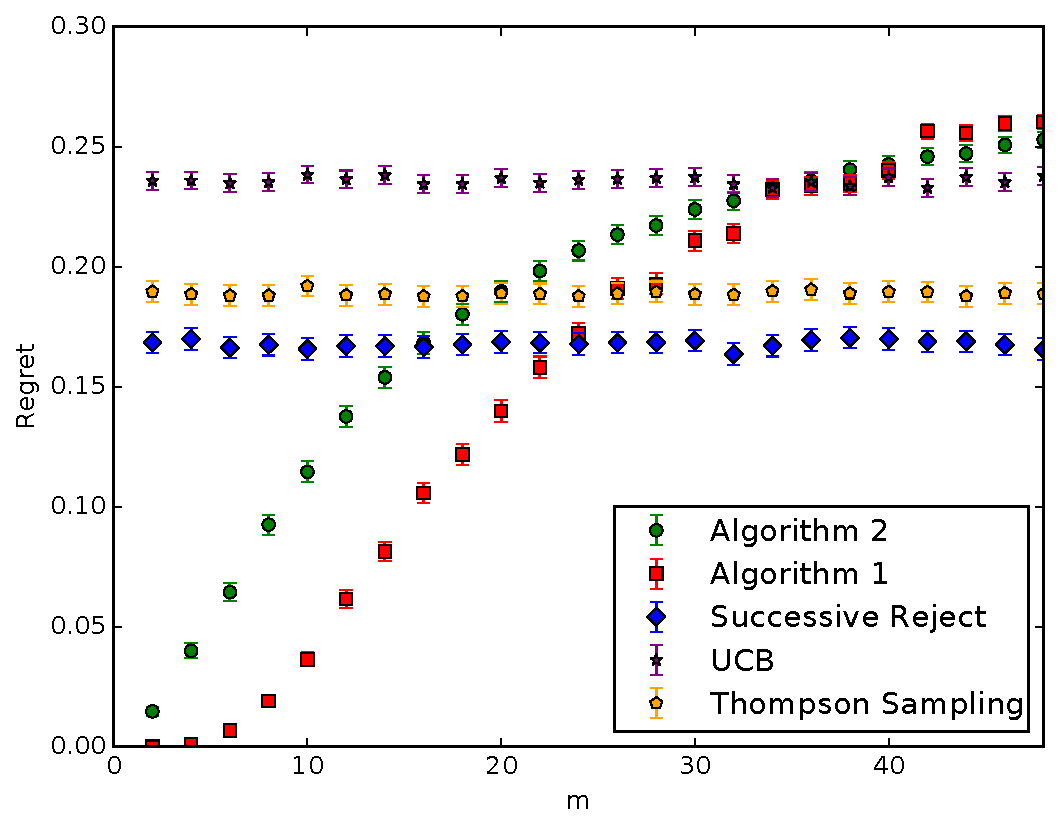
\includegraphics[width=\textwidth]{experiment1_20161020_1247.pdf}
    		\caption{Simple regret vs $m(\boldsymbol{q})$ for fixed horizon $T=400$ and number of variables $N = 50$}
        \label{fig:simple_vs_m}
    \end{subfigure}\hfill
    \begin{subfigure}[t]{0.3\textwidth}
    		\centering
        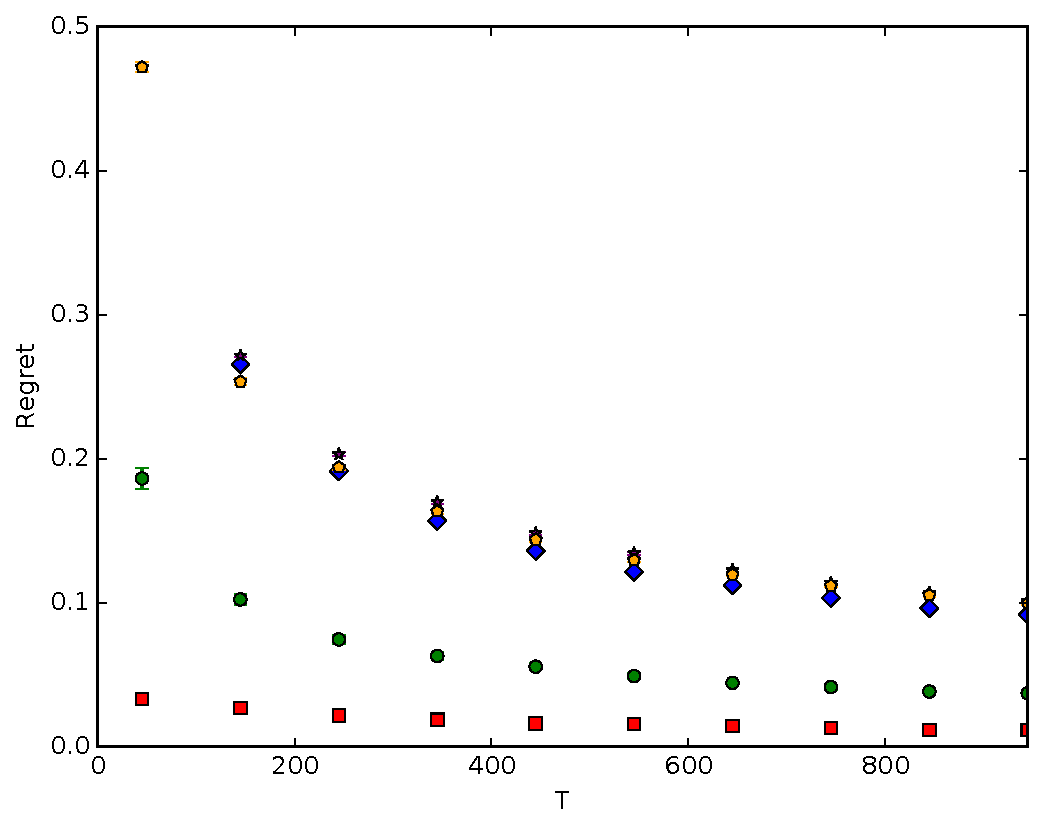
\includegraphics[width=\textwidth]{experiment2_20161020_1249.pdf}
    		\caption{Simple regret vs horizon, $T$, with $N = 50$, $m=2$ and $\epsilon = \sqrt{\frac{N}{8T}}$}
        \label{fig:simple_vs_T_vary_epsilon}
    \end{subfigure}\hfill
    \begin{subfigure}[t]{0.3\textwidth}
    		\centering
    		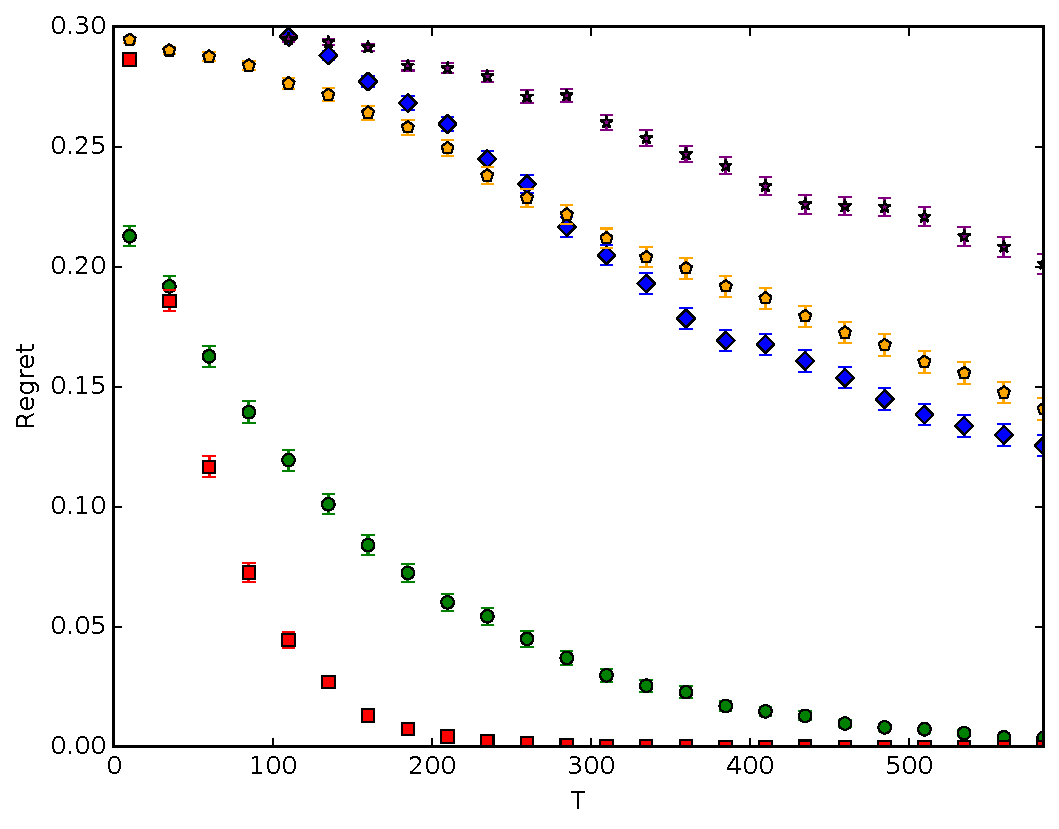
\includegraphics[width=\textwidth]{experiment3_20161020_1252.pdf}
    		\caption{Simple regret vs horizon, $T$, with $N = 50$, $m=2$ and fixed $\epsilon = .3$}
    		\label{fig:simple_vs_T}
    \end{subfigure}
    \caption{Experimental results}
    \label{fig:experiments}
\end{figure}

Figure \ref{fig:simple_vs_T_vary_epsilon} demonstrates the performance of the algorithms in the worst case environment for standard bandits, where the gap between the optimal and sub-optimal arms, $\smash{\epsilon = \sqrt{N/(8T)}}$ , is just too small to be learned. This gap is learn-able by the causal algorithms, for which the worst case $\epsilon$ depends on $m \ll N$. In Figure \ref{fig:simple_vs_T} we fix $N$ and $\epsilon$ and observe that, for sufficiently large $T$, the regret decays exponentially. The decay constant is larger for the causal algorithms as they have observed a greater effective number of samples for a given $T$. 

For the parallel bandit problem, the regression estimator used in the specific algorithm outperforms the truncated importance weighted estimator in the more general algorithm, despite the fact the specific algorithm must estimate $\boldsymbol{q}$ from the data. 
This is an interesting phenomenon that has been noted before in off-policy evaluation where the regression (and not the importance weighted) estimator is known to be mini-max optimal asymptotically \citep{li2014minimax}.


\begin{figure}[H]
	\centering    
          \begin{tikzpicture}[->,>=stealth',shorten >=1pt,auto,node distance=.45cm,
  thick,main node/.style={observed}, hidden/.style={empty},background rectangle/.style={fill=olive!45}]
%every node/.style={scale=0.6}
 %nodes
\node[main node](1){$X_{1}$};
\node[main node, right=of 1](2){$X_{2}$};
\node[hidden, right=of 2](3){$...$};
\node[main node, right=of 3](4){$X_{N}$};
\node[main node, below right=of 2](5){$Y$};
\node[main node, above right=of 2](6){$Z$};
 \path[every node/.style={font=\tiny}]
    (1) edge (5)
    	(2) edge (5)
    (4) edge (5)
    (6) edge (1) edge (2) edge (4);
\end{tikzpicture}
        \caption{Confounded graph}
        \label{fig:parallel_confounded} 
\end{figure}


We now compare the general algorithm with a range of standard bandit algorithms on the confounded graph in Figure \ref{fig:parallel_confounded}. All the variables are binary and the action space consists of the set of single variable interventions plus the do nothing action, 

\eq{
\calA = \set{\set{do(X_i = j)} \cup \set{do(Z = j)} \cup \set{do()}: 1\leq i \leq N,\; j \in \set{0,1}}
} 

We choose this setting because it generalises the parallel bandit, while simultaneously being sufficiently simple that we can compute the exact reward and interventional distributions for large $N$ (in general inference in graphical models is exponential in $N$). As before, we show the average regret over 10,000 simulations with error bars showing three standard errors. 

In Figure \ref{fig:simple_vs_m_general} we fix $N$ and $T$ and $P(Z=1) = .4$. For some $2 \leq N_1 \leq N$ we define 
\eq{
P(X_i = 1|Z = 0) &= \begin{cases} 0 & \text{ if } i \in \set{1,...N_1} \\ .4 & \text{ otherwise } \end{cases}\\
P(X_i = 1|Z = 1) &= \begin{cases} 0 & \text{ if } i \in \set{1,...N_1} \\ .65 & \text{ otherwise } \end{cases}
}
As in the parallel bandit case, we let $Y$ depend only on $X_1$, $P(Y|do(X_1=1)) = \frac{1}{2} + \epsilon$ and $P(Y|do(X_1=0)) = \frac{1}{2}-\epsilon'$, where $\epsilon' = \epsilon P(X_1=1) / P(X_1=0)$. The value of $N_1$ determines $m$ and ranges between $2$ and $N$. The values for the CPD's have been chosen such that the reward distribution is independent of $m$ and so that we can analytically calculate $\eta*$. This allows us to just show the dependence on $m$, removing the noise associated with different models selecting values for $\eta*$ with the same $m$ (and also worst case performance), but different performance for a given reward distribution. 

In Figure \ref{fig:simple_vs_T_general} we fix the model and number of variables, $N$, and vary the horizon $T$. $P(Z)$ and $P(X|Z)$ are the same as for the previous experiment.  
In Figure \ref{fig:simple_vs_T_misspecified} we additionally show the performance of Algorithm 1, but exclude actions on $Z$ from the set of allowable actions to demonstrate that Algorithm 1 can fail in the presence of a confounding variable, which occurs because it incorrectly assumes that $P(Y|do(X)) = P(Y|X)$. 
We let $P(Z) = .6$, $P(Y|\boldsymbol{X}) = X_7 \oplus X_N$ and $P(X|Z)$ be given by:

\eq{
P(X_i = 1|Z = 0) &= 
\begin{cases} 
.166 & \text{ if } i \in \set{1,..., 6} \\
.2 & \text{ if } i = 7 \\
.7 & \text { otherwise} 
 \end{cases}\\
 P(X_i = 1|Z = 1) &= 
\begin{cases} 
.166 & \text{ if } i \in \set{1,..., 6} \\
.8 & \text{ if } i = 7 \\
.3 & \text { otherwise} 
 \end{cases}\\
}

In this setting $X_7$ tends to agree with $Z$ and $X_N$ tends to disagree. It is sub-optimal to act on either $X_7$ or $X_N$, while all other actions are optimal. The first group of $X$ variables with $i \leq 6$ will be identified by the parallel bandit as the most unbalanced ones and played explicitly. All remaining variables are likely to be identified as balanced and estimated from observational estimates. The CPD values have been chosen to demonstrate the worst case outcome, where the bias in the estimates leads Algorithm 1 to asymptotically select a sub-optimal action.

\begin{figure}[H]
    \begin{subfigure}[t]{0.3\textwidth}
		\centering    
    		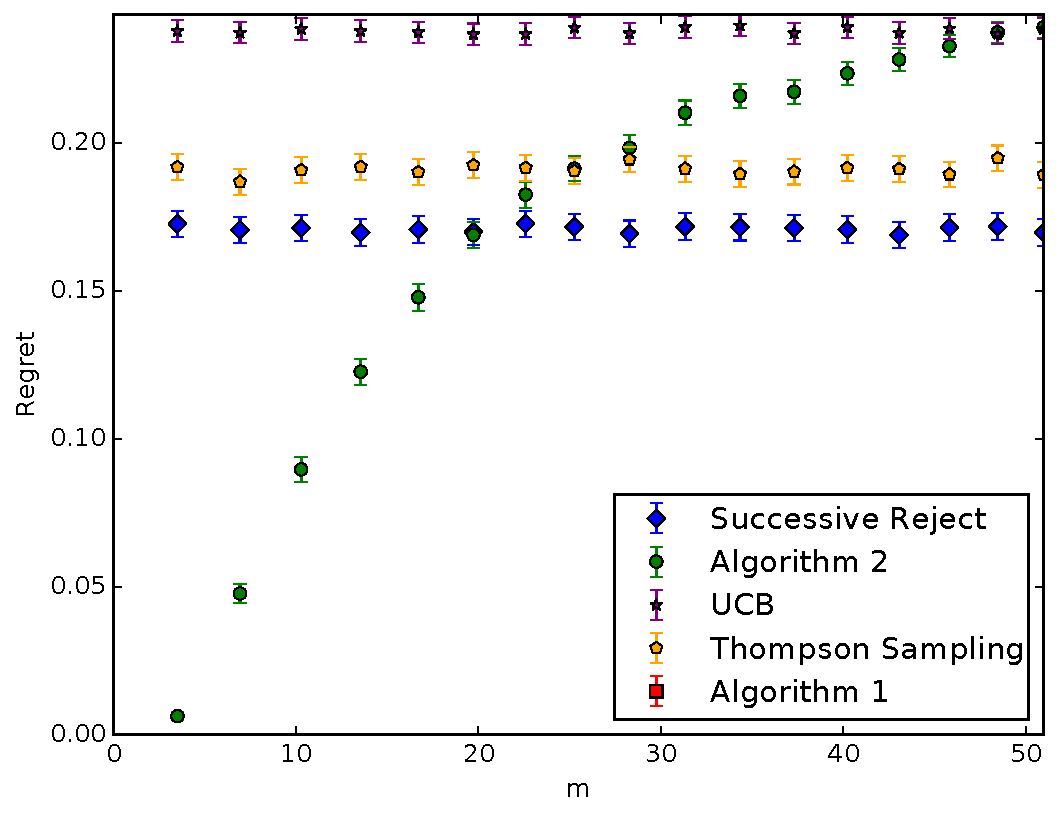
\includegraphics[width=\textwidth]{experiment4_20161023_2120.pdf}
    		\caption{Simple regret vs $m(\eta*)$ for fixed horizon $T=400$ and number of variables $N = 50$}
        \label{fig:simple_vs_m_general}
    \end{subfigure}\hfill
    \begin{subfigure}[t]{0.3\textwidth}
    		\centering
        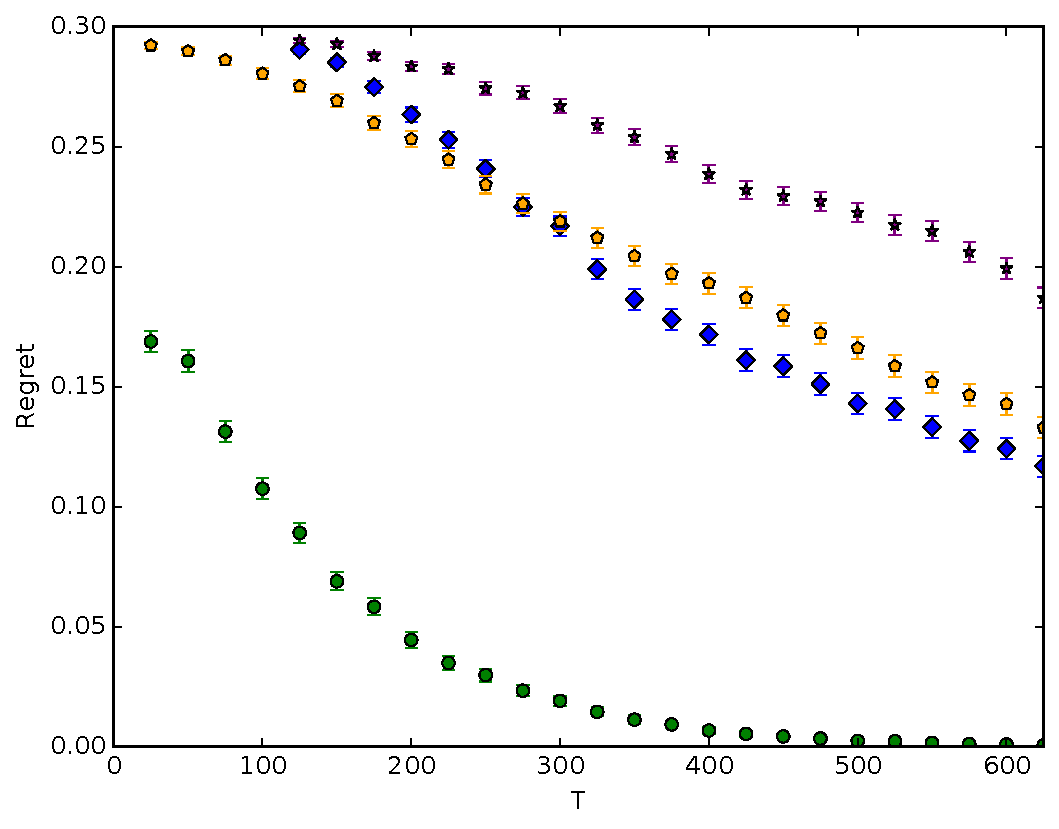
\includegraphics[width=\textwidth]{experiment7_20161020_1257.pdf}
    		\caption{Simple regret vs horizon, $T$, with $N = 50$ and $m(\eta*)=3.1$ }
        \label{fig:simple_vs_T_general}
    \end{subfigure}\hfill
    \begin{subfigure}[t]{0.3\textwidth}
    		\centering
    		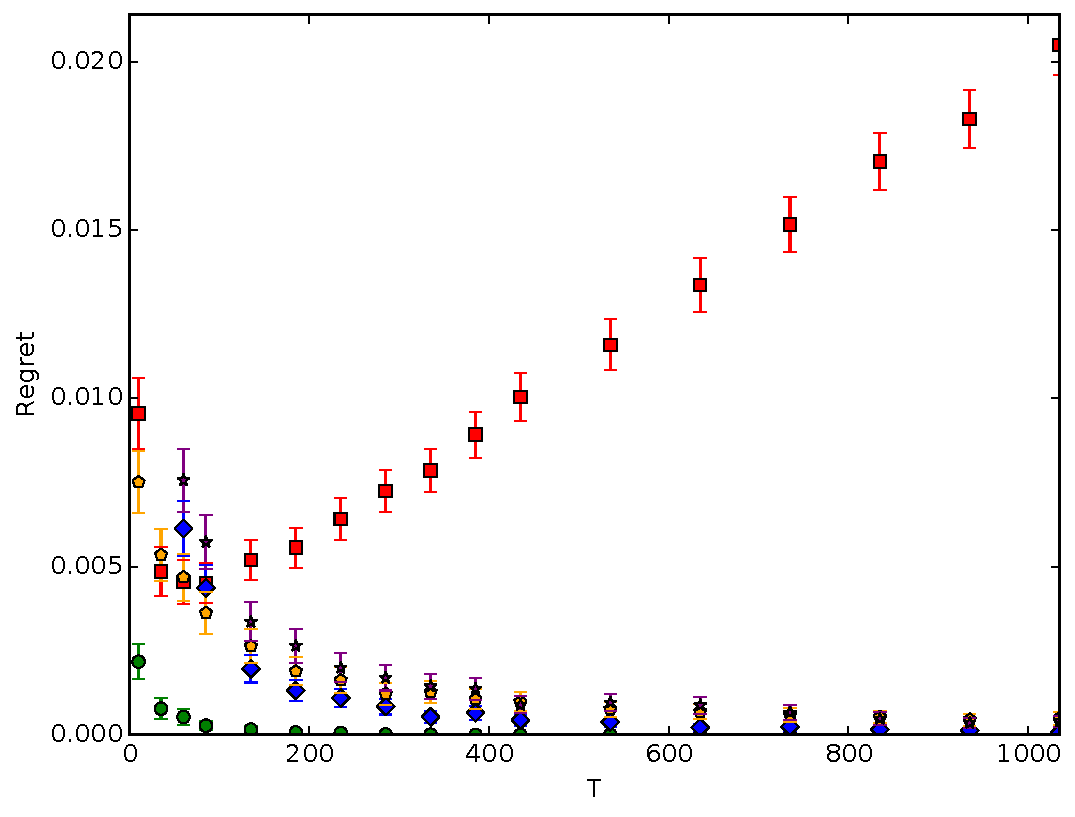
\includegraphics[width=\textwidth]{experiment5_20161023_2118.pdf}
    		\caption{Simple regret vs horizon, $T$, with $N = 21$, $m(\eta*)=4.3$ with no actions setting $Z$}
    		\label{fig:simple_vs_T_misspecified}
    \end{subfigure}
    \caption{Experimental results on the confounded graph}
    \label{fig:experiments_confounded}
\end{figure}

\subsection{Discussion \& Future work}
\label{sec:causal_bandit_discussion}
Algorithm~\ref{alg:general} for general causal bandit problems 
estimates the reward for all allowable interventions $a \in \calA$ over $T$ rounds by sampling and applying interventions from a distribution $\eta$.
Theorem~\ref{thm:general} shows that this algorithm has (up to log factors) simple regret that is $\smash{\mathcal O(\sqrt{m(\eta)/T)}}$ where 
the parameter $m(\eta)$ measures the difficulty of learning the causal model and is always less than $N$.
The value of $m(\eta)$ is a uniform bound on the variance of the reward estimators $\hat{\mu}_a$ and, intuitively, problems where all variables' values in the causal model ``occur naturally'' when interventions are sampled from $\eta$ will have low values of $m(\eta)$.

The main practical drawback of Algorithm~\ref{alg:general} is that both the estimator $\hat{\mu}_a$ and the optimal sampling distribution $\eta^*$ (\ie, the one that minimises $m(\eta)$) require knowledge of the conditional distributions $\Pn{a}{\parents{Y}}$ for all $a \in \calA$. In contrast, in the special case of parallel bandits, Algorithm~\ref{alg:simple} uses the $do()$ action to effectively estimate $m(\eta)$ and the rewards then re-samples the interventions with variances that are not bound by $\hat{m}(\eta)$.
Despite these extra estimates, Theorem~\ref{thm:lower} shows that this approach is optimal (up to log factors).Finding an algorithm that only requires the causal graph and lower bounds for its simple regret in the general case is left as future work.


\paragraph{Making Better Use of the Reward Signal}
Existing algorithms for best arm identification are based on ``successive rejection'' (SR) of arms based on UCB-like bounds on their rewards~\citep{Even-Dar2002}. In contrast, our algorithms completely ignore the reward signal when developing their arm sampling policies and only use the rewards when estimating $\hat{\mu}_a$. Incorporating the reward signal into our sampling techniques or designing more adaptive reward estimators that focus on high reward interventions is an obvious next step. This would likely improve the poor performance of our causal algorithm relative to the successive rejects algorithm for large $m$, as seen in Figure~\ref{fig:simple_vs_m}.

For the parallel bandit the required modifications should be quite straightforward. The idea would be to adapt the algorithm to essentially use successive elimination in the second phase so arms are eliminated as soon as they are provably no longer optimal with high probability. In the general case a similar modification is also possible by dividing the budget $T$ into phases and optimising the sampling distribution $\eta$, eliminating arms when their confidence intervals are no longer overlapping. This has now been done by \citet{Sen2017a}, leading to problem dependent regret bounds for causal bandit problems. Note that these modifications do not improve the mini-max regret, which at least for the parallel bandit is already optimal. For this reason we focused on emphasising the point that causal structure can and should be exploited when available. Another observation is that Algorithm \ref{alg:general} is actually using a fixed design, which in some cases may be preferred to a sequential design for logistical reasons. This is not possible for Algorithm \ref{alg:simple}, since the $\vec{q}$ vector is unknown.

\paragraph{Cumulative Regret}
Although we have focused on simple regret in our analysis, it would also be natural to consider the cumulative regret. In the case of the parallel bandit problem we can slightly modify the analysis from \citep{wu2015online} on bandits with side information 
to get near-optimal cumulative regret guarantees. They consider a finite-armed bandit model with side information where in reach round the learner chooses an action and receives a Gaussian reward signal for all actions, but with a known variance that depends on the chosen action. In this way the learner can gain information about actions it does not take with varying levels of accuracy. The reduction follows by substituting the importance weighted estimators in place of the Gaussian reward. In the case that $\vec{q}$ is known this would lead to a known variance and the only (insignificant) difference is the Bernoulli noise model. In the parallel bandit case we believe this would lead to near-optimal cumulative regret,
at least asymptotically. 

%Their model assumes the rewards for all arms $a$ are Gaussian with mean $\mu_a$ and variance $\sigma^2_{ab}$ and that playing an arm $a$ will reveal a side observation $Y_{ab}$ of the reward for all arms $b$ distributed with mean $\mu_b$ and variance $\sigma^2_{ab}$.
%We can build a similar dependence structure with variances for a Bernoulli reward variable that is derived from the $\vec{q}$ vector of probabilities.
%\todom{Check this!}
%Even though the original results are for Gaussian rewards we believe the analysis will go through largely unchanged.

The parallel bandit problem can also be viewed as an instance of a time varying graph feedback problem \citep{Alon2015,Kocak2014}, where at each time step the feedback graph $G_t$ is selected stochastically, dependent on $\boldsymbol{q}$, and revealed after an action has been chosen. The feedback graph is distinct from the causal graph. A link $A \rightarrow B$ in $G_t$ indicates that selecting the action $A$ reveals the reward for action $B$. For this parallel bandit problem, $G_t$ will always be a star graph with the action $do()$ connected to half the remaining actions. However, \citet{Alon2015,Kocak2014} give adversarial algorithms, which when applied to the parallel bandit problem obtain the standard bandit regret. A malicious adversary can select the same graph each time, such that the rewards for half the arms are never revealed by the informative action. This is equivalent to a nominally stochastic selection of feedback graph where $\boldsymbol{q} = \boldsymbol{0}$. 

\citet{Lelarge2012} consider a stochastic version of the graph feedback problem, but with a fixed graph available to the algorithm before it must select an action. In addition, their algorithm is not optimal for all graph structures and fails, in particular, to provide improvements for star like graphs as in our case. \citep{Buccapatnam2014} improve the dependence of the algorithm on the graph structure but still assume the graph is fixed and available to the algorithm before the action is selected. 



\paragraph{Causal Models with Non-Observable Variables}
If we assume knowledge of the conditional \textit{interventional} distributions $\Pn{a}{\parents{Y}}$ our analysis applies unchanged to the case of causal models with 
non-observable variables. Some of the interventional distributions may be non-identifiable meaning we can not obtain prior estimates for $\Pn{a}{\parents{Y}}$ from 
even an infinite amount of observational data. Even if all variables are observable and the graph is known, if the conditional distributions are unknown, then Algorithm
\ref{alg:general} cannot be used. Estimating these quantities while simultaneously minimising the simple regret is an interesting and challenging open problem.

% For example, if we had access to a data set of \textit{experiments} in which the reward variable $Y$ was not available from which to build estimates of $P_a$.
% In this case, some conditional distributions may be non-identifiable. 
% The corresponding actions can be immediately added to the set $A$ prior to collecting any data. 
% We can then use the same algorithm as in the case where there are no latent variables, except that we will have to use the more general do-calculus rather than simply adjusting for the parents to write the expression for each action in terms of observational data.
% Combining our estimation techniques with insights from \citet{Bareinboim2015} for handling unobserved confounders would be worth investigation.


% More generally, assuming causal structure creates more complex types of side information, such as that shown in equation \ref{eq:estimation_transfer}. In this case, selecting one action does not fully reveal an alternate action but provides some information towards an estimate. The quality of the estimate notably depends not only on the number of times that action was selected. For example, to get a good estimate for $X_1 = 1$ by intervening on $X_2$ requires us to sample both $X_2=0$ and $X_2=1$, in proportions dependent on $q_2$. This more complex side information does not fit within the graph feedback framework.


\paragraph{Partially or Completely Unknown Causal Graph}
A much more difficult generalisation would be to consider causal bandit problems where the causal graph is completely unknown or known to be a member of class of models.
The latter case arises naturally if we assume free access to a large observational data set, from which the Markov equivalence class can be found via causal discovery techniques. 
Work on the problem of selecting experiments to discover the correct causal graph from within a Markov equivalence class~\citep{eberhardt2005,eberhardt2010causal,hauser2014two,Hu2014} could potentially be incorporated into a causal bandit algorithm.
In particular, \citet{Hu2014} show that only $\bigo{\log \log n}$ multi-variable interventions are required on average to recover a causal graph over $n$ variables once purely observational data is used to recover the ``essential graph''.
Simultaneously learning a completely unknown causal model while estimating the rewards of interventions without a large observational data set would be much more challenging.

\subsection{Proofs}
\subsubsection{Proof of Theorem \ref{thm:uq-simple}}\label{sec:thm:uq-simple}


Assume without loss of generality that $q_1 \leq q_2 \leq \ldots \leq q_N \leq 1/2$. The assumption is non-restrictive since all variables
are independent and permutations of the variables can be pushed to the reward function. 

The proof of Theorem \ref{thm:uq-simple} requires some lemmas. \

\begin{lemma}\label{lem:conc1}
Let $i \in \set{1,\ldots, N}$ and $\delta > 0$. Then
\eq{
\P{\left|\hat q_i - q_i\right| \geq \sqrt{\frac{6q_i}{T} \log \frac{2}{\delta}}} \leq \delta\,.
}
\end{lemma}

\begin{proof}
By definition, $\hat{q}_i = \frac{2}{T}\sum_{t=1}^{T/2}X_{t,i}$, where $X_{t,i} \sim Bernoulli(q_i)$. Therefore from the Chernoff bound (see equation 6 in \citet{Hagerup1990}),

\eq{
\P{\left|\hat q_i - q_i\right| \geq \epsilon} \leq 2e^{-\frac{T\epsilon^2}{6q_i}}
}

Letting $\delta = 2e^{-\frac{T\epsilon^2}{6q_i}}$ and solving for $\epsilon$ completes the proof.

\end{proof}

\begin{lemma}\label{lem:m_est}

Let $\delta \in (0,1)$ and assume $T \geq 48m \log\frac{2N}{\delta}$. Then
\eq{
\P{2m(\vec{q}) / 3 \leq m(\vec{\hat q}) \leq 2m(\vec{q})} \geq 1 - \delta\,.
}
\end{lemma}

\begin{proof}
Let $F$ be the event that there exists and $1 \leq i \leq N$ for which
\eq{
\left|\hat q_i - q_i\right| \geq \sqrt{\frac{6q_i}{T} \log \frac{2N}{\delta}}\,.
}
Then by the union bound and Lemma \ref{lem:conc1} we have $\P{F} \leq \delta$. The result will be completed by showing that
when $F$ does not hold we have $2m(\vec{q})/3 \leq m(\vec{\hat q}) \leq 2m(\vec{q})$.
From the definition of $m(\vec{q})$ and our assumption on $\vec{q}$ we have for $i > m(\vec{q})$ that $q_i \geq q_m \geq 1/m(\vec{q})$ and so by Lemma \ref{lem:conc1} we have
\eq{
\frac{3}{4} 
&\geq \frac{1}{2} + \sqrt{\frac{3}{T} \log \frac{2N}{\delta}} 
\geq q_i + \sqrt{\frac{6q_i}{T} \log \frac{2N}{\delta}} 
\geq \hat q_i \\
&\geq q_i - \sqrt{\frac{6q_i}{T} \log \frac{2N}{\delta}}
\geq q_i - \sqrt{\frac{q_i}{8m(\vec{q})}}
\geq \frac{1}{2m(\vec{q})}\,.
}
Therefore by the pigeonhole principle we have $m(\vec{\hat q}) \leq 2m(\vec{q})$.
For the other direction we proceed in a similar fashion. Since the failure event $F$ does not hold we have for $i \leq m(\vec{q})$ that
\eq{
\hat q_i 
\leq q_i + \sqrt{\frac{6q_i}{T} \log\frac{2N}{\delta}} 
\leq \frac{1}{m(\vec{q})} \left(1 + \sqrt{\frac{1}{8}}\right)
\leq \frac{3}{2m(\vec{q})}\,.
}
Therefore $m(\vec{\hat q}) \geq 2m(\vec{q}) / 3$ as required. 
\end{proof}

\begin{proof}[Proof of Theorem \ref{thm:uq-simple}]
Recall that $A = \set{a \in \actions : \hat p_a \leq 1/m(\vec{\hat q})}$. Then,
for $a \in A$, the algorithm estimates $\mu_a$ from $T_A \doteq T/(2m(\vec{\hat q}))$ samples. From lemma \ref{lem:m_est}, $T_A  \geq T/(4m(\vec{q}))$ with probability $(1-\delta)$. Let $H$ be the event $T_A < T/(4m(\vec{q}))$ and $G$ be the event $\exists a \in A : |\mu_a - \hat \mu_a| \geq \sqrt{\frac{2m(\vec{q})}{T} \log\frac{2N}{\delta}}$

\eq{
\P{G} \leq \P{H} + \P{G|\neg H} \leq \delta + \P{G|\neg H}
}

Via Hoeffding's inequality and the union bound, 

\eq{
\P{G|\neg H}&\doteq \P{\exists a \in A : |\mu_a - \hat \mu_a| \geq \sqrt{\frac{2m(\vec{q})}{T} \log\frac{2N}{\delta}},\text{ given }T_A \geq T/(4m(\vec{q}))} \leq \delta\\
 \implies  \P{G} & \doteq \P{\exists a \in A : |\mu_a - \hat \mu_a| \geq \sqrt{\frac{2m(\vec{q})}{T} \log\frac{2N}{\delta}}} \leq 2\delta\,.
}
For arms not in $A$,

\eq{
\hat p_a = & \frac{2}{T} \sum_{t=1}^{T/2} \ind{X_i = j} \geq 1/m(\vec{\hat q}), \; \text {by definition of not being in $A$}\\
 \geq & \frac{1}{2m(\vec{q})},\; \text{ with probability } 1-\delta \\
\implies  T_a \doteq & \sum_{t=1}^{T/2} \ind{X_i = j} \geq  \frac{T}{4m(\vec{q})},\; \text{ with probability } 1-\delta
}

Again applying Hoeffding's and the union bound

\eq{
\P{\exists a \notin A:  \left|\hat \mu_a - \mu_a\right| \geq \sqrt{\frac{2m(\vec{q})}{T} \log \frac{2N}{\delta}}} \leq 2\delta
}


Therefore, combining this result with the bound for arms $a \in A$, we have with probability at least $1 - 4\delta$ that,
\eq{
(\forall a \in \actions) \qquad |\hat \mu_a - \mu_a| \leq \sqrt{\frac{2m(\vec{q})}{T} \log \frac{2N}{\delta}} \doteq \epsilon\,.
}
If this occurs, then 
\eq{
\mu_{\hat a^*_T} \geq \hat \mu_{\hat a^*_T} - \epsilon \geq \hat \mu_{a^*} - \epsilon \geq \mu_{a^*} - 2\epsilon\,.
}
Therefore
\eq{
\mu^* - \EE[\mu_{\hat a^*_T}] 
& \leq 4\delta + \epsilon\\
& \leq \frac{8m(\vec{q})}{T} + \sqrt{\frac{2m(\vec{q})}{T} \log \frac{NT}{m(\vec{q})}},\; \text{ letting } \delta = \frac{2m(\vec{q})}{T}\\
& \leq \sqrt{\frac{20m(\vec{q})}{T} \log \frac{NT}{m(\vec{q})}},\; \text{ via Jenson's Inequality}
}
which completes the result.
\end{proof}

%%%%%%%%%%%%%%%%%%%%%%%%%%%%%%%%%%%%%%%%%%%%
% LOWER BOUND
%%%%%%%%%%%%%%%%%%%%%%%%%%%%%%%%%%%%%%%%%%%%
\subsubsection{Proof of Theorem \ref{thm:lower}}\label{sec:thm:lower}

We follow a relatively standard path by choosing multiple environments that have different optimal arms, but which cannot all be statistically
separated in $T$ rounds.
Assume without loss of generality that $q_1 \leq q_2 \leq \ldots \leq q_N \leq 1/2$.
For each $i$ define reward function $r_i$ by
\eq{
r_0(\boldsymbol{X}) &= \frac{1}{2} &
r_i(\boldsymbol{X}) &= \begin{cases}
\frac{1}{2} + \epsilon & \text{if } X_i = 1 \\
\frac{1}{2} & \text{otherwise}\,,
\end{cases}
}
where $1/4 \geq \epsilon > 0$ is some constant to be chosen later.
We abbreviate $R_{T,i}$ to be the expected simple regret incurred when interacting with the
environment determined by $\boldsymbol{q}$ and $r_i$. Let $\operatorname{P}_i$ be the corresponding measure
on all observations over all $T$ rounds and $\EE_i$ the expectation with respect to $\operatorname{P}_i$. By Lemma 2.6 by \citet{Tsy08} we have
\eq{
\Prz{\hat a^*_T = a^*} + \Pri{\hat a^*_T \neq a^*} \geq \exp\left(-\KL(\operatorname{P}_0, \operatorname{P}_i)\right)\,,
}
where $\KL(\Ps_0, \Ps_i)$ is the KL divergence between measures $\operatorname{P}_0$ and $\operatorname{P}_i$.
Let $T_i(T) = \sum_{t=1}^T \ind{a_t = do(X_i = 1)}$ be the total number of times the learner intervenes on variable $i$ by setting it to $1$.
Then for $i \leq m$ we have $q_i \leq 1/m$ and the KL divergence between $\Ps_0$ and $\Ps_i$ may be bounded using the telescoping property (chain rule) and
by bounding the local KL divergence by the $\chi$-squared distance as by \citet{Auer1995}. This leads to 
\eq{
\KL(\Ps_0, \Ps_i) 
&\leq 6\epsilon^2 \EE_0\left[\sum_{t=1}^T \ind{X_{t,i} = 1}\right] 
\leq 6\epsilon^2 \left(\EE_0 T_i(T) + q_i T\right) 
\leq 6\epsilon^2 \left(\EE_0 T_i(T) + \frac{T}{m}\right)\,.
}
Define set $A = \set{i \leq m : \EE_0 T_i(T) \leq 2T / m}$.
Then for $i \in A$ and choosing $\epsilon = \min\set{1/4, \sqrt{m/(18T)}}$ we have
\eq{
\KL(\Ps_0, \Ps_i) \leq \frac{18T\epsilon^2}{m} = 1\,. 
}
Now $\sum_{i=1}^m \EE_0 T_i(T) \leq T$, which implies that $|A| \geq m/2$.
Therefore
\eq{
\sum_{i \in A} \Pri{\hat a^*_T \neq a} 
\geq \sum_{i \in A} \exp\left(-\KL(\Ps_0, \Ps_i)\right) - 1
\geq \frac{|A|}{e} - 1 
\geq \frac{m}{2e} - 1\,.
}
Therefore there exists an $i \in A$ such that
$\Pri{\hat a^*_T \neq a^*} \geq \frac{\frac{m}{2e} - 1}{m}$. 
Therefore if $\epsilon < 1/4$ we have
\eq{
R_{T,i} \geq \frac{1}{2} \Pn{i}{\hat a^*_T \neq a^*} \epsilon \geq \frac{\frac{m}{2e} - 1}{2m} \sqrt{\frac{m}{18T}}\,.
}
Otherwise $m \geq 18T$ so $\sqrt{m/T} = \Omega(1)$ and
\eq{
R_{T,i} \geq \frac{1}{2} \Pn{i}{\hat a^*_T \neq a^*} \epsilon \geq \frac{1}{4} \frac{\frac{m}{2e} - 1}{2m} \in \Omega(1) 
}
as required.

%%%%%%%%%%%%%%%%%%%%%%%%%%%%%%%%%%%%%%%%%%%%
% GENERAL-GRAPH UPPER BOUND
%%%%%%%%%%%%%%%%%%%%%%%%%%%%%%%%%%%%%%%%%%%%
\subsubsection{Proof of Theorem \ref{thm:general}}\label{sec:thm:general}

\begin{proof}
First note that $X_t, Y_t$ are sampled from $\operatorname{Q}$.
We define $Z_a(X_t) = Y_t R_a(X_t)\ind{R_a(X_t)\leq B_a}$ and abbreviate $Z_{at} = Z_a(X_t)$, $R_{at} = R_a(X_t)$ and $\Pn{a}{.} = \Pns{a}{.}$.
By definition we have $|Z_{at}| \leq B_a$ and 
\eq{
\Var_Q[Z_{at}] 
\leq \EE_Q[Z_{at}^2] 
\leq \EE_Q[R_{at}^2]
= \EEa[R_{at}]
= \EEa\left[\frac{\Pns{a}{\parents{Y}(X)}}{\Q{\parents{Y}(X)}}\right] 
\leq m(\eta)\,.
}
Checking the expectation we have
\eq{
\EE_Q[Z_{at}] 
= \EEa \left[Y \ind{R_{at} \leq B_a}\right] 
= \EEa Y - \EEa \left[Y\ind{R_{at} > B_a}\right] 
= \mu_a - \beta_a\,,
}
where 
\eq{
0 \leq \beta_a = \EEa[Y \ind{R_{at} > B_a}] \leq \Pns{a}{R_{at} > B_a}
}
is the negative bias. 
The bias may be bounded in terms of $m(\eta)$ via an application of Markov's inequality.
\eq{
\beta_a \leq \Pns{a}{R_{at} > B_a} \leq \frac{\EEa[R_{at}]}{B_a} \leq \frac{m(\eta)}{B_a}\,.
}
Let $\epsilon_a > 0$ be given by
\eq{
\epsilon_a = \sqrt{\frac{2m(\eta)}{T} \log\left(2T|\calA|\right)} + \frac{3B_a}{T} \log\left(2T|\calA|\right)\,.
}
Then by the union bound and Bernstein's inequality 
\eq{
\P{\text{exists } a \in \calA : \left|\hat \mu_a - \EE_Q[Z_{at}]\right| \geq \epsilon_a} 
\leq \sum_{a \in \calA} \P{\left|\hat \mu_a - \EE_Q[Z_{at}]\right| \geq \epsilon_a} \leq \frac{1}{T}\,.
}

Let $I = \hat{a}^*_T$ be the action selected by the algorithm, $a^* = \argmax_{a \in \calA} \mu_a$ be the true optimal action and recall that $\EE_Q[Z_{at}] = \mu_a - \beta_a$. Assuming the above event does not occur we have,

\eq{
\mu_I \geq \hat \mu_I - \epsilon_I  
\geq \hat \mu_{a^*} - \epsilon_I  
\geq \mu^* - \epsilon_{a^*} - \epsilon_I - \beta_{a^*}\,. 
}
By the definition of the truncation
we have
\eq{
\epsilon_a \leq \left(\sqrt{2} + 3\right)\sqrt{\frac{m(\eta)}{T} \log\left(2T|\calA|\right)}
}
and
\eq{
\beta_a \leq \sqrt{\frac{m(\eta)}{T} \log\left(2T|\calA|\right)}\,. 
}
Therefore for $C = \sqrt{2} + 4$ we have
\eq{
\P{\mu_I \geq \mu^* - C \sqrt{\frac{m(\eta)}{T} \log\left(2T|\calA|\right)}} \leq \frac{1}{T}\,.
}
Therefore
\eq{
\mu^* - \EE[\mu_I] \leq C \sqrt{\frac{m(\eta)}{T} \log\left(2T|\calA|\right)} + \frac{1}{T}
}
as required.
\end{proof}

\subsubsection{Relationship between $m(\eta)$ and $m(\boldsymbol{q})$}\label{sec:m-equivelence}

\begin{proposition} In the parallel bandit setting,
$m(\eta^*) \leq 2m(\boldsymbol{q})$.
\end{proposition} 

\begin{proof}

Recall that in the parallel bandit setting,

\eq{
\mathcal{A} = \set{do()} \cup \set{ do(X_i = j) \colon 1 \leq i \leq N \text{ and } j \in \set{0,1}}
}

Let:

\eq {
\eta_a = \ind{\P{X_i = j} < \frac{1}{m(\boldsymbol{q})}}\frac{1}{2m(\boldsymbol{q})} \text { for } a \in do(X_i = j)
}

Let $D =\sum_{a\in do(X_i=j)}\eta_a$. From the definition of $m(\boldsymbol{q})$, 
\eq {
\sum_{a\in do(X_i=j)} \ind{\P{X_i = j} < \frac{1}{m(\boldsymbol{q})}} \leq m(\boldsymbol{q}) \implies D \leq \frac{1}{2}
}
 
Let $\eta_a = \frac{1}{2} + (1-D)$ for $a = do()$ such that $\sum_{a \in \calA}\eta_a = 1$ 

Recall that,

\eq{
m(\eta) &
= \max_a \EEa\left[\frac{\Pn{a}{\parents{Y}(X)}}{\Q{\parents{Y}(X)}}\right]
}

We now show that our choice of $\eta$ ensures $\EEa\left[\frac{\Pn{a}{\parents{Y}(X)}}{\Q{\parents{Y}(X)}}\right] \leq 2m(\boldsymbol{q})$ for all actions $a$.

For the actions $a: \eta_a > 0$, ie $do()$ and $do(X_i = j):\P{X_i=j}<\frac{1}{m(\boldsymbol{q})}$,
\eq{
\EEa\left[\frac{\Pn{a}{X_1...X_N}}{\sum_{b}\eta_b\Pn{b}{X_1...X_N}}\right] \leq \EEa\left[\frac{\Pn{a}{X_1...X_N}}{\eta_a\Pn{a}{X_1...X_N}}\right] = \EEa\left[\frac{1}{\eta_a}\right] \leq 2m(\boldsymbol{q})
}

For the actions $a :\eta_a = 0$, ie $do(X_i=j):\P{X_i=j}\geq\frac{1}{m(\boldsymbol{q})}$,
\eq{
\EEa\left[\frac{\Pn{a}{X_1...X_N}}{\sum_{b}\eta_b\Pn{b}{X_1...X_N}}\right] \leq & \EEa\left[\frac{\ind{X_i=j}\prod_{k\neq i}\P{X_k}}{(1/2+D)\prod_k \P{X_k}}\right] \\=& \EEa\left[\frac{\ind{X_i=j}}{(1/2+D)\P{X_i = j}}\right]
\leq  \EEa\left[\frac{\ind{X_i=j}}{(1/2)(1/m(\boldsymbol{q}))}\right] \leq 2m(\boldsymbol{q})
}

Therefore $m(\eta*) \leq m(\eta) \leq 2m(\boldsymbol{q})$ as required.

\end{proof}


\chapter{Conclusion}

The underlying motivation behind much applied statistical and machine learning work is to guide us to make better decisions. In many cases, the actions that we take in response to the model will change the system from which the data was generated. It is critical that we are able to recognise the causal nature of such problems and appropriately model the decision making part of the process. If machine learning is to be as transformative in fields such as economics, medicine and social science as it has been for image recognition, voice processing and machine translation, we must develop methods to estimate the effect of, and optimally select, interventions that are as effective as those we have for pattern recognition. We need to bridge the gap between the theory driven models of economics and science and the black box prediction approach that has been so successful in machine learning. This will involve clarifying what information is (currently) best encoded by theory and what can be successfully inferred from data and developing methods that can incorporate the theory or structure required to allow models to generalise from one setting to another whilst retaining the flexibility to capture complex patterns in empirical data. 

A better understanding of causality is also relevant for the discussions around transparency and ethics in machine learning, particularly with respect to the European Union's new General Data Protection Regulation, which requires that automated decision systems that significantly affect individuals provide provide \textit{"meaningful information about the logic involved."} \cite{Goodman2016}. The recognition that there is a fundamental trade-off between accuracy and transparency, unless we can build perfect causal models, when the interests of individuals and society diverge has implications for they way we design and regulate systems that have the potential to have major impacts on people's lives. We must develop approaches to ensuring machine learning decisions are reasonable and ethical that allow effected individuals recourse to dispute or improve outcomes but do not undermine the ability of the system to function. 

The observational and interventional viewpoints on learning to act contribute complementary components to a general approach. Observational causal inference provides, through the do-calculus, a formal means to map information from observational to interventional settings, as well as between different interventions. Bandit algorithms, capture the sequential nature of decision making processes and provide techniques to carefully balance exploration and exploitation. 

I have developed a framework that formally connects causal graphical models with bandit problems in a very natural way and demonstrated that this framework encode some key existing problems in the literature. I showed that knowledge of the causal structure (but not the functional relationships) between variables can induce a novel form of structure between alternate actions and that an algorithm that leverages this structure obtains better performance that one that does not. 

This work represents an important first step towards a unified approach to causal inference and optimal decision making. There is much exciting work remaining to be done. Although the causal bandit framework can capture contextual information as well as post-action feedback, I have formally analysed and developed algorithms only for the latter. Additionally, to make the problem tractable, I made the (major) assumption that the interventional distribution over the parents of the outcome was known. This can be relaxed to assuming the interventional distribution over some Markov blanket with respect to the outcome is known. Information can then be shared between actions outside the blanket in the same way as in algorithm \ref{alg:general}, whilst actions inside could be learned explicitly. Relaxing this assumption entirely is a much more challenging problem. However, as is demonstrated by the specific example of the parallel causal bandit problem, it is possible to develop algorithms that require only the casual structure of the graph and yield substantially lower regret.

Another interesting line of research is the question of off-policy evaluation for causal-bandit problems. As in the online case, knowledge of the causal structure between variables in the graph provides additional information about the reward for the actions that were not selected at each timestep. The problem differs from typical observational causal inference in several ways; the focus is on identifying an optimal policy, rather than unbiased estimation of all policies, the goal is to explore the value of interventions on a range of different variables, rather than the optimal setting of a single variable, and the data will, in general, be non-stationary in a rather special way due to the adaptive nature of policy that generated it. Existing work on off-policy evaluation focuses (at least implicitly) on estimating causal effects by adjusting for all variables that simultaneously effect both the action selection and outcome. If additional information is available about the causal relationships between variables involved, other approaches to identifying causal effects such as instrumental variables or the \quotes{front door method} \citep{Pearl2000} could be also be applied to off-policy evaluation. 

Insights from the bandit literature can also be applied to more classical causal inference problems. In particular, estimators that are geared towards optimal action selection (rather than evaluation of all actions) and approaches to quantify the finite time properties, as opposed to asymptotic efficiency, of estimators, for example \citep{li2014minimax}.  
 
An important line of research, that is relevant to both the observational and interventional approaches to causal inference, is developing methodologies for model evaluation and selection that provide something equivalent to what cross-validation does for supervised learning. 

My hope is that in the next years, combining the reinforcement learning approach to decision making, with causal graphical models and causal effect estimation techniques developed within statistics and economics, will revolutionise our ability to make good data driven decisions. 

\bibliographystyle{apalike}% Select the citation style e.g. ieeetr
\bibliography{library}% write the directory to the .bib file
\end{document}

\chapter{Causation vs Prediction}


Mixing continuous experimentation at an individual level with batch approaches. There may be fixed costs associated with \quotes{enabling} certain actions. For example, social programs may have some fixed overheads, no matter how many people are enrolled in them, etc. Reuse data obtained to optimise for one outcome to learn about optimising for another. We don't have a single outcome or loss-measure that fully incorporates everything we care about for the majority of problems.

The two cultures \citep{Breiman2001}
 - wrong because suggests we can just use the machine learning approach for everything. Does not address the problems that a) structural assumptions required for causal inference. b) we cannot use cross-validation to assess the validity of a causal model (really b is the whole point).


To explain or to predict \citep{Shmueli2010}
- wrong because they assume all the parts of explanatory modelling are required - so black box models cannot be used. 



Predict the relationship between X and Y as a way to stratify to reduce the variance in an experiment.

They consider a different definition of explanatory models, 

Definition as backwards. Explanatory models focus on theory because some theory (or equivalently stated assumptions) are required in order to predict the outcome of an intervention from observational data. 

Causal modelling frameworks allow us to separate assumptions about the structure of the relationships between variables from assumptions about the functional form. 

What can be data driven and what cannot? (for a given set of assumptions). 


Allowing for the possibility that we might only need to be able to predict the outcome of an intervention on a given subset of variables (for example those over which we have the ability to manipulate) or the possibility that we can can obtain observation from directly intervening in a system creates creates a need for models that are neither explanatory or predictive in the language of EoP but are built on a hybrid of both approaches. 


